% !TeX spellcheck = en_US
% !TeX program = pdflatex
%\RequirePackage{pkgloader} % Deals with order in which packages need to be loaded
\documentclass[11pt, a4paper, english]{report}
%\RequirePackage[l2tabu, orthodox]{nag}
\usepackage{babel}
\usepackage{microtype}
\usepackage{etex}
\usepackage[margin=1in]{geometry}
\usepackage[utf8]{inputenc}
\usepackage[T1]{fontenc}
\usepackage{graphicx}
\usepackage[ddmmyyyy]{datetime}
\usepackage{amsfonts}
\usepackage{newtxtext}
\usepackage{amsmath}
\usepackage{amssymb}
\usepackage{bm}
\usepackage{mathtools}
\usepackage{lettrine}		%For big letters (i.e. dropped capitals) when starting a new chapter
\usepackage{enumerate}
\usepackage{multicol}
\usepackage{etoolbox}
\usepackage{adjustbox}
\usepackage[dvipsnames, table]{xcolor}

\usepackage{ntheorem}
\usepackage{float}
\usepackage{subfig}
\usepackage{caption}

% For load order, see https://tex.stackexchange.com/questions/24586/how-to-hyperref-a-pageref-in-second-half-of-an-algorithm-independent-of-first-h
\usepackage[hypertexnames=false]{hyperref}  % needed to help hyperlinks direct correctly;
\usepackage[all]{hypcap}
\usepackage[chapter]{algorithm}
\usepackage{algorithmicx, algpseudocode}

\usepackage{cryptocode}
\usepackage{booktabs}
\usepackage{pdftexcmds}
\usepackage[newfloat]{minted}
\usepackage{mathpartir}
\usepackage{mathrsfs}

\usepackage{fancyhdr}
\usepackage{tikz}
\usepackage{textcomp}
\usepackage{xpatch}
\usepackage{gensymb}
\usepackage{marvosym}
\usepackage{tikz}
\usepackage{bytefield}

\usepackage{physics}

\usepackage{cancel}
\usepackage{tikz}
\usepackage{pgfplots}

\usepackage[noabbrev,capitalize]{cleveref}
\usepackage[ocgcolorlinks]{ocgx2} % See https://tex.stackexchange.com/a/230762 , prevents the colors from references and such from being printed on actual paper

%\LoadPackagesNow % pkgloader: load the packages

% Enabling some tikz libararies
\usetikzlibrary{automata, positioning, arrows, calc, intersections, through, backgrounds, tikzmark}
\pgfplotsset{compat=1.12}

%Default minted style
\setminted{style=default}

%%%%%%%%%%%%%%%%%%%%%%%%%%%%%%%%%%%%%%%%%%%%%%
% Minted Source Code Spanning Multiple Pages %
%%%%%%%%%%%%%%%%%%%%%%%%%%%%%%%%%%%%%%%%%%%%%%%%%%%%%%%%%%%%%%%%%%%%%%%%%%%%%%%%%%%%%%%
% @see http://tex.stackexchange.com/questions/254044/caption-and-label-on-minted-code %
%%%%%%%%%%%%%%%%%%%%%%%%%%%%%%%%%%%%%%%%%%%%%%%%%%%%%%%%%%%%%%%%%%%%%%%%%%%%%%%%%%%%%%%
\newenvironment{code}{\captionsetup{type=listing}}{}
\SetupFloatingEnvironment{listing}{name=Listing}


%%%%%%%%%%%%%%%%%%%%%%
% Royal Initialen Font %
%%%%%%%%%%%%%%%%%%%%%%
\input RoyalIn.fd
\newcommand*\initfamily{\usefont{U}{RoyalIn}{xl}{n}}


%%%%%%%%%%%%
% Settings %
%%%%%%%%%%%%
\graphicspath{{img/}}
\captionsetup{hypcap=false}

%%%%%%%%%%%%%%%%%%%%%%%%%%%%%%%%%
% Break theorem after its label %
%%%%%%%%%%%%%%%%%%%%%%%%%%%%%%%%%
\theoremstyle{break}



%%%%%%%%%%%%%%%%%%%%%%%%
% Algo in/out redefine %
%%%%%%%%%%%%%%%%%%%%%%%%
\renewcommand{\algorithmicrequire}{\textbf{Input: }}
\renewcommand{\algorithmicensure}{\textbf{Output: }}

%%%%%%%%%%%%%%%%%%%%%%%%%%%%%%%%%%%%%%%%%%%%%%%%%%%%%%%%%%%%%%%%%%%%%%%%%%%%%%%%%%%%%%%%%%%%%%%%%%%%%%
% Custom colors for hyperref																		 %	
% @see https://tex.stackexchange.com/questions/100905/best-practice-for-hyperref-link-colours/102068 %
%%%%%%%%%%%%%%%%%%%%%%%%%%%%%%%%%%%%%%%%%%%%%%%%%%%%%%%%%%%%%%%%%%%%%%%%%%%%%%%%%%%%%%%%%%%%%%%%%%%%%%
\newcommand\myshade{85}
\colorlet{mylinkcolor}{violet}
\colorlet{mycitecolor}{YellowOrange}
\colorlet{myurlcolor}{Aquamarine}

\hypersetup{
	linkcolor  = mylinkcolor!\myshade!black,
	citecolor  = mycitecolor!\myshade!black,
	urlcolor   = myurlcolor!\myshade!black,
	colorlinks = true,
}

%%%%%%%%%%
% Macros %
%%%%%%%%%%
\newcommand{\fourq}{Four$\mathbb{Q}$}
\newcommand{\fourqs}{Four$\mathbb{Q}$'s}

%%%%%%%%%%%%%%%%%%%%%%%%%%%
% Lemma's and definitions %
%%%%%%%%%%%%%%%%%%%%%%%%%%%
\newtheorem{lemma}{Lemma}
\newtheorem{definition}{Definition}
\newtheorem{theorem}{Theorem}

% For citing RFC's, see this tool:
% http://notesofaprogrammer.blogspot.nl/2014/11/bibtex-entries-for-ietf-rfcs-and.html

%%%%%%%%%%%%%%%%%%
% Tikz functions %
%%%%%%%%%%%%%%%%%%
\pgfmathdeclarefunction{gauss}{2}{%
	\pgfmathparse{1/(#2*sqrt(2*pi))*exp(-((x-#1)^2)/(2*#2^2))}%
}

%%%%%%%%%%%%%%%%%%%%%%%%%%%%%%%%%%%%%%%%%%%%%%%%%%%%%%%%%%%%%%%%%%%%%%%%%%%%%
% Disable PDF inclusion warnings, see https://tex.stackexchange.com/a/78020 %
%%%%%%%%%%%%%%%%%%%%%%%%%%%%%%%%%%%%%%%%%%%%%%%%%%%%%%%%%%%%%%%%%%%%%%%%%%%%%
\pdfsuppresswarningpagegroup=1


\begin{document}	
	% !TeX spellcheck = en_US
% !TeX root = ../Tom_Sandmann-research_internship_plan
\begin{titlepage}
	\begin{center}
		\textsc{\Huge Master Thesis\\Computer Science}\\[1.5cm]
		
\includegraphics[height=100pt]{front/logo}\\
		\vspace{0.4cm}
		\textsc{\Large Radboud University}\\[1cm]
		\vspace{0.4cm}
		\textbf{\huge  Online Template Attack on a Hardware Implementation of \fourq}\\[0.4cm]
		\vspace{2cm}
		\begin{minipage}[t]{0.45\textwidth}
			\begin{flushleft} \large
				\textit{Author}\\
				Tom Sandmann\\
				s4330048
			\end{flushleft}
		\end{minipage}
		\begin{minipage}[t]{0.45\textwidth}
			\begin{flushright} \large
				\textit{First supervisor \& assessor}\\
				Dr. Lejla Batina\\
				lejla@cs.ru.nl \\[1.3cm]
				\textit{Second assessor}\\
				MSc. Pedro Maat C. Massolino \\
				p.massolino@cs.ru.nl
			\end{flushright}
		\end{minipage}
		\vfill
		{\large 07/08/2018}
	\end{center}
\end{titlepage}
	
	
	\clearpage
	\hypersetup{pageanchor=false}
	% !TeX spellcheck = en_US
% !TeX root = ../Tom_Sandmann-master_thesis
\begin{abstract}
Electronic devices can perform all sorts of operations which we can analyze.
We can either analyze a single operation executed by the device, or a full execution.
Side-channel attacks (SCAs) exploit the relation between information leaked through a side-channel and the corresponding secret data.
Different types of side-channels can be used: timing information, power consumption and electromagnetic signals are all information sources that can be used in SCAs.
When we consider an implementation on a specific device, we can use these side channels to obtain secret information stored or used in this device. 
This can break secrecy assumptions about confidential information used in these devices.
In Elliptic Curve Cryptography (ECC), we use public and private keys to encrypt and decrypt messages.
If we have an encrypted message, the original message can only be obtained if one knows the corresponding private key.
Construction of these keys depends on a problem that makes it particularly hard to obtain the private key assuming  the public key is accessible to anyone.
With respect to ECC, the difficulty of this problem depends on the intractability of determining $k$ from $Q = kP$ where the points $P$ and $Q$ are known. 
This computation of $kP$ is also known as scalar multiplication.
In \cite{costello2015fourq}, a new curve called {\fourq} is introduced.
Scalar multiplication on {\fourq} is very fast compared to other curves that were considered after its introduction.
This is because {\fourq} can make use of a 4-dimensional Gallant-Lambert-Vanstone (GLV) decomposition, which reduces the total number of operations needed to compute a scalar multiplication.
In this thesis, we attack a hardware implementation of {\fourq} on FPGAs which was introduced in \cite{jarvinen2016four}.
We make use of an Online Template Attack (OTA) \cite{batina2014online}, which greatly reduces the number of templates needed compared to regular template attacks. 
\end{abstract}
	% !TeX spellcheck = en_US
% !TeX root = ../Tom_Sandmann-master_thesis
\renewcommand{\abstractname}{Acknowledgements}
\begin{abstract}
	First I would like to thank my supervisors Lejla Batina and Pedro Massolino for granting me the opportunity to work on this project. In particular I would like to thank Pedro for his time and patience to answer my (sometimes) endless stream of questions, helping me in the lab setting up the equipment and bringing up suggestions when I was facing difficult problems.
	I would also like to thank Matthias and Abdullah for our amazing times at both the TU/e and the RU.
	In addition, I also want to thank all the people from NSN with whom I have had a great time with. 
	Finally, I would like to thank my parents for their support throughout the years of studying in Nijmegen.
	Without all of you, I would not have been the person I have become now.
\end{abstract}
	\hypersetup{pageanchor=true}
	\clearpage
	
	\microtypesetup{protrusion=false}
	\tableofcontents
	\microtypesetup{protrusion=true}
	
	% !TeX spellcheck = en_US
% !TeX root = ../Tom_Sandmann-master_thesis
\chapter{Introduction}
\lettrine[lhang = 0.4, findent=-30pt, lines=4]{\textbf{
		\initfamily \fontsize{20mm}{20mm} \selectfont I
		\normalfont}}{n}
public key cryptography, the cryptographic system has a pair of keys: the public and private key.
The public key can be distributed freely, while the private key must remain known only to the owner.
If this is the case, authentication, encryption and non-repudiation can be achieved.
We introduce to three major families of public-key algorithms based on their underlying computational problem \cite{paar2009understanding}:
%
\begin{itemize}
	\item \textbf{Integer-Factorization Schemes:} schemes based on the fact that large integers are hard to factor. An example of a scheme that falls into this category is RSA.
	
	\item  \textbf{Discrete Logarithm Schemes:} schemes based on the discrete logarithm problem in groups. An example of a scheme that falls into this category is the Diffie-Hellman key exchange.
	 
	\item \textbf{Elliptic Curve Schemes}: A generalization of the discrete logarithm algorithm are elliptic curve public-key schemes. An example of a scheme that falls into this category is the Elliptic Curve Diffie-Hellman key exchange (ECDH).
\end{itemize}
\parshape=0
%
An advantage of Elliptic Curve Cryptography (ECC) is the fact that it can offer the same level of security while using much smaller parameters than non-ECC cryptography.
This leads to a significant increase in performance and makes these algorithms more suitable for (embedded) systems where amount of memory is limited and where energy consumption should be minimal.

A Field-Programmable Gate Array (FPGA) is an integrated circuit that is designed to be configurable after it has been manufactured.
FPGAs have become an attractive option for deploying hardware applications in comparison to the well-established Application-Specific Integrated Circuits (ASICs).
Besides their great flexibility, FPGAs also reduce the development costs and allow for faster prototyping.
For these reasons, FPGAs have become targets for many ECC implementations \cite{guneysu2008ultra, sasdrich2014efficient, sasdrich2015implementing}.

In \cite{costello2015fourq}, a new elliptic curve with the name {\fourq} is proposed. 
This curve provides approximately 128 bits of security.
By combining a four-dimensional decomposition wit the fastest (explicit) twisted Edwards curves formulas available and in combination with the efficient Mersenne prime $p = 2^{127} - 1$, it supports highly-efficient scalar multiplications.
For generic scalar multiplications, {\fourq} performs four to five times faster than the original NIST P-256 curve \cite{costello2015fourq, gueron2015fast}, and is also faster than curves that were considered as NIST alternatives after its introduction.
In \cite{jarvinen2016four}, an implementation of {\fourq} on FPGAs is proposed, which was the first time {\fourq} was implemented and deployed on reconfigurable hardware.
As expected, the speed results of the hardware design of {\fourq} are positive: a speedup factor of 2-2.5 was observed on a Xillinx Zynq-7020 FPGA, in comparison with the corresponding variants of the fastest Curve22519 implementation on the same device.
The proposed {\fourq} hardware implementation exhibits constant time execution, which protects against timing and simple side channel attacks.
This enables us to test the resistance of the proposed hardware implementation against other, more advanced, side channel attacks (see \Cref{chp: Side Channel Attacks}).

\section{Related Work}
Side-channels rely on the relation between information leaked through a side-channel and the secret data related to this information. 
A frequent used side-channel is the power consumption of a device.
A simple attack that makes use of this information is simple power analysis (SPA), in which the power consumption of a device is visually examined.
This enables an adversary to observe the different operations occurring in the execution of the algorithm.
If the algorithm does not run in constant time, the graph of the power consumption can be used to retrieve the secret data in the execution of the algorithm.
This type of attack is however hard to perform in practice, as countermeasures against SPA are generally fairly simple to implement.
A more advanced side-channel attack is differential power analysis (DPA), in which power consumption measurements are statistically analyzed \cite{kocher1999differential}.
This requires a large number of power traces from the same device using the same secret.
The more traces we capture, the higher the chances of successfully performing the attack.
The number of traces required is related to the noise that is inherent to captured power traces.
DPA requires multiple power traces for the same secret, which is something that cannot always be realized in practice.
Therefore, new techniques that fall between SPA and DPA have been developed, with one of the most notable ones being template attacks \cite{chari2002template, rechberger2004practical, choudary2013efficient}.
Template attacks are generally used to attack the secret scalar in a scalar multiplication algorithm.
This attack only requires one target trace to attack this secret, while numerous template traces are needed in the precomputation phase.
This type of attack was improved in \cite{batina2014online}, in which Online Template Attacks (OTAs) were introduced and successfully applied.
OTAs reduce the number of templates and only require one target trace from the device under attack.
These are horizontal SCAs, in which different parts of the same trace are considered to attack different key bits.
The OTA applied in the original paper was used to attack different scalar multiplication algorithms that executed in constant-time.
In addition, different input representations (i.e. affine and projective) for these algorithms were also considered.
They only attacked the first 5 bits of the scalar due to a problem in their measurement setup.
However, a complete key retrieval using an OTA was performed in \cite{dugardin2016dismantling}.
In this paper, the open-source cryptographic library PolarSSL, that can be used in embedded devices, was attacked.
The implementation was modified to speed up the finite field computations.
Simply put, they made use of leakage due to a potential overflow in the field multiplication.
To increase the success rate of the template matching phase, they averaged multiple traces for a single template.
This increased the correlation value of the correct template from 69\% (when only using 1 template trace) to 99.8\% (when using the average of 100 template traces). 
The correlation value was calculated using the Pearson correlation coefficient.
However, the chance of retrieving the 256-bit scalar when using 100 additional template traces per trace still remains low.
Due to their approach, they were however able to correct and detect errors in attacking a single key-bit with reasonable probability.
This made full scalar retrieval very likely.

Most of the published power analysis attacks are applied to smart card and microcontrollers.
\cite{ors2003power} is one of the first papers in which a simple power-analysis attack was applied to FPGAs.
In this paper, a Montgomery modular multiplier implementation (without the final subtraction) on a FPGA was attacked.
The attack involved a visual inspection of the computation power trace, which clearly showed the secret key.
In \cite{standaert2004power}, a DPA attack was applied to a FPGA running a DES implementation. 
As mentioned in this paper, the physical behavior of FPGAs is different than smart cards.
Therefore, the original proposal of DPA and its improvements were not directly applicable to FPGAs.
This was dealt with by generalizing the power model of the attack to account for this difference in physical behavior.
The proposed techniques were successfully applied to DES, and it was also verified that other block ciphers (including AES Rijndael) were vulnerable to the proposed methods.
In \cite{guntur2014side}, a new FPGA board called SAKURA-G was introduced that contains two Spartan-6 FPGAs.
The SAKURA-G board was evaluated by making use of a correlation power analysis (CPA) on an AES circuit with no countermeasures against SCAs.
Results of this power analysis were compared to the previously introduced standard boards SASEBO-GII and SASEBO-G.
The CPA on each of the boards was conducted five times without changing the conditions and using the same key and plaintext.
It was shown that the SAKURA-G board reduced the number of templates needed to successfully perform a CPA by half compared to the other boards \cite{guntur2014side}. 
In addition, power traces captured using the SAKURA-G board were cleaner compared to the other boards. 
These results make the SAKURA-G board a good option when you want to verify the protection of hardware designs against side-channel attacks.

In \cite{costello2015fourq}, a fast curve named {\fourq} was introduced that provides a very fast way to perform scalar multiplication.
An implementation of {\fourq} on microcontrollers with strong countermeasures against side-channel attacks was presented in \cite{liu2017fourq}. 
The countermeasures in this implementation applied to a variety of side-channel attacks, and should increase the difficulty for an attacker to successfully apply an unprofiled vertical attack.
The effectiveness of the countermeasures was partially verified by carrying out a DPA evaluation using a discovery board containing the ARM Cortex-M4 microcontroller. 


\section{Outline Thesis}
In this section, we describe the outline for the rest of this thesis.
In \Cref{chp: SAKURA-G} we provide information about the board that is used to run the hardware implementation of {\fourq} and to capture the power traces necessary to perform the side-channel attack: the Side-channel AttacK User Reference Architecture
Board (SAKURA-G) \cite{guntur2014side}.
This includes details about how the data is transmitted from and to the board and which state machines and interfaces are used to realize this.
Information about elliptic curves is summarized in \Cref{chp: Elliptic Curves}.
In \Cref{chp: FourQ}, we describe the details of the curve {\fourq}.
Details regarding the hardware implementation of {\fourq} are discussed in \Cref{chp: FourQ On Hardware}.
\Cref{chp: Side Channel Attacks} contains details about (online) template attacks.
The application of an OTA to {\fourq} and the corresponding results are described in \Cref{chp: Attacking FourQ}.
\Cref{chp: Conclusion and Discussion} concludes and discusses this thesis.

	% !TeX spellcheck = en_US
% !TeX root = ../Tom_Sandmann-master_thesis
\chapter{SAKURA-G} \label{chp: SAKURA-G}
\lettrine[lhang = 0.4, findent=-30pt, lines=4]{\textbf{
		\initfamily \fontsize{20mm}{20mm} \selectfont T
		\normalfont}}{he}
SAKURA-G board consists of two integrated Spartan-6 FPGAs.
One of these Spartan FPGAs serves as the main security circuit (XC6SLX75-2CSG484C), while the other one serves as the controller (XC6SLX9-2CSG225C). 
The main Spartan contains the actual cryptographic hardware design.
The control Spartan is used to control the main board by changing specific signals received by the main board (e.g. signals indicating whether encryption/decryption has to be performed, or whether the internal state has to be reset). 
To deploy a hardware design on our FPGA, we need to somehow transfer this design to the board.
This requires the hardware design to be processed in a specific way:
% https://www.xilinx.com/itp/xilinx10/isehelp/ise_c_implement_fpga_design.htm
\begin{enumerate}
	\item \textbf{Synthesis}: the abstract description of our hardware design (written in for example VHDL or Verilog) is turned into a design implementation of logic gates and lookup tables (LUTs), digital signal processors (DSPs), BRAMs and other elements.
	
	\item \textbf{Mapping, Place and Route}: the structures identified in the previous step are mapped to FPGA elements.
	These components are then routed and the appropriate signals are connected.
	
	\item \textbf{Program file}: a file is generated that can be transferred to the FPGA. Depending on the file format, this file either gets flashed to the flash memory on the SAKURA-G board, or is stored in the FPGA non-persistent memory.
\end{enumerate}
%

\section{Constraints}
Constraints are used to guide the design tool on how specific parts of the design should be treated. There are two types of constraints:
%
\begin{itemize}
	\item \textbf{Synthesis constraints} are used by the synthesis tool to optimize specific parts of the hardware description language (HDL) code. 
	They can be either embedded directly within the VHDL/Verilog code or specified in an external synthesis constraint file.
	
	\item \textbf{Implementation constraints} are instructions passed to FPGA implementation tools that specify mapping, placement, timing and other guidelines followed by the implementation tool while processing a FPGA design. These constraints are generally placed in a User Constraint File (\texttt{UCF}). Examples of these constraints are \texttt{LOC} (placement) and \texttt{PERIOD} (timing) constraints. In the hardware design we consider, the majority of the constraints (if not all) are \texttt{LOC} constraints. \texttt{LOC} constraints define where a design element can be placed within a FPGA. 
\end{itemize}
%

\section{JTAG}
JTAG was a standard initially developed by IEEE to solve issues with electronically manufactured boards. 
It is a standard used to verify designs and circuit board after they have been manufactured.
In our case, it is used as a programming, debug and probing port. 
The JTAG programmer/debugger is attached to both the JTAG port and the micro-USB port, which makes it ready to use. 
We use the JTAG programmer to load hardware designs of the control and main FPGAs to the Spartan FPGAs.
In general, there are two file formats that can be loaded to a FPGA:
%
\begin{itemize}
	\item \texttt{BIT} file: A \texttt{.BIT} file is a raw storage of the programming bits for the FPGA.
	It can be loaded to the FPGA via JTAG using for example \texttt{iMPACT} (a Xilinx specific utility).
	This file format is primarily used for testing a hardware design. The reason for this is, when the board loses its power, the design is ``lost''.
	
	\item \texttt{MCS} file: A \texttt{.MSC} file is flashed to flash memory, which means that the contents are not lost when power is lost. The \texttt{.MSC} file can be flashed to flash-memory via JTAG using \texttt{iMPACT}. On power-up, specific configuration signals are used to load the program to the board.
\end{itemize}
%

% !TeX spellcheck = en_US
% !TeX root = ../Tom_Sandmann-master_thesis
\section{Interface with the board} \label{sec: Interface with the board}
To interface with the Spartan FPGAs that are present on the SAKURA-G, we make use of Python code from the ChipWhisperer project%
\footnote{\url{https://newae.com/tools/chipwhisperer/}}.
In addition, we make use of the source files for both the main and control FPGAs available on the SAKURA-G website%
\footnote{\url{http://satoh.cs.uec.ac.jp/SAKURA/hardware/SAKURA-G.html}}.
The software needed to develop and deploy hardware designs to our board is as follows:
%
\begin{itemize}
	\item Xilinx ISE 14.7 (licensed);
	\item FTDI drivers D2XX%
	\footnote{\url{http://www.ftdichip.com/Drivers/D2XX.htm}};
	\item FT PROG%
	\footnote{\url{http://www.ftdichip.com/Support/Utilities.htm\#FT_PROG}}.
\end{itemize}
%
The FTDI drivers are required by the \texttt{ftd2xx} Python package to send and receive data to and from one of the FPGAs (i.e. either the control or the main FPGA).
\mintinline{text}{FT_PROG} can be used to view connected FPGAs (if any).
Finally, Xilinx ISE is used to generate the corresponding program files for our design and send them to the board. 

We now describe the structure of the interfaces used in the designs of the control and main FPGAs.
The two FPGAs on the SAKURA-G board are interconnected through a local bus.
The SAKURA-G makes use of an USB FTDI interface that allows an external PC to communicate with the one of the FPGAs.
Channel A of the the USB interface (FT2232H) is connected to the controller FPGA and channel B is connected to the main FPGA.
Depending on the DIP switch (and another control flag), we are connected to either the main FPGA or to the control FPGA.
As we do not need to directly interface with the main FPGA, we assume to be always connected to the USB interface of the control FPGA.

The control FPGA can send and receive data to the main FPGA by making use of the local bus.
The control FPGA also receives external inputs such as a 48MHz clock and a reset signal.
In addition, it can also control the LEDs that are located next to the FPGA on the board.
The 48MHz clock that is received as input by the control FPGA is used to generate two clocks:
one that is used as the system clock (\texttt{clk}), and another one (\mintinline{text}{usb_clk}) to clock the USB connection (which by default is clocked at 24MHz).
The system clock is used in both the local bus (connecting the two FPGAs) and in the main FPGA.
The frequency at which the system clock operates is controlled by the (4-bit wide) User DIP switch (where the default operation frequency is 1.5MHz).
To make use of a different operation frequency, we set the first bit of the DIP switch to high.
The remaining bits of this switch control the new frequency (3, 6, 12 or 24MHz).
A schematic overview of the connection between the two boards can be seen in \Cref{fig: sakura_g-signal-overview}.
%
\begin{figure}
	\centering
	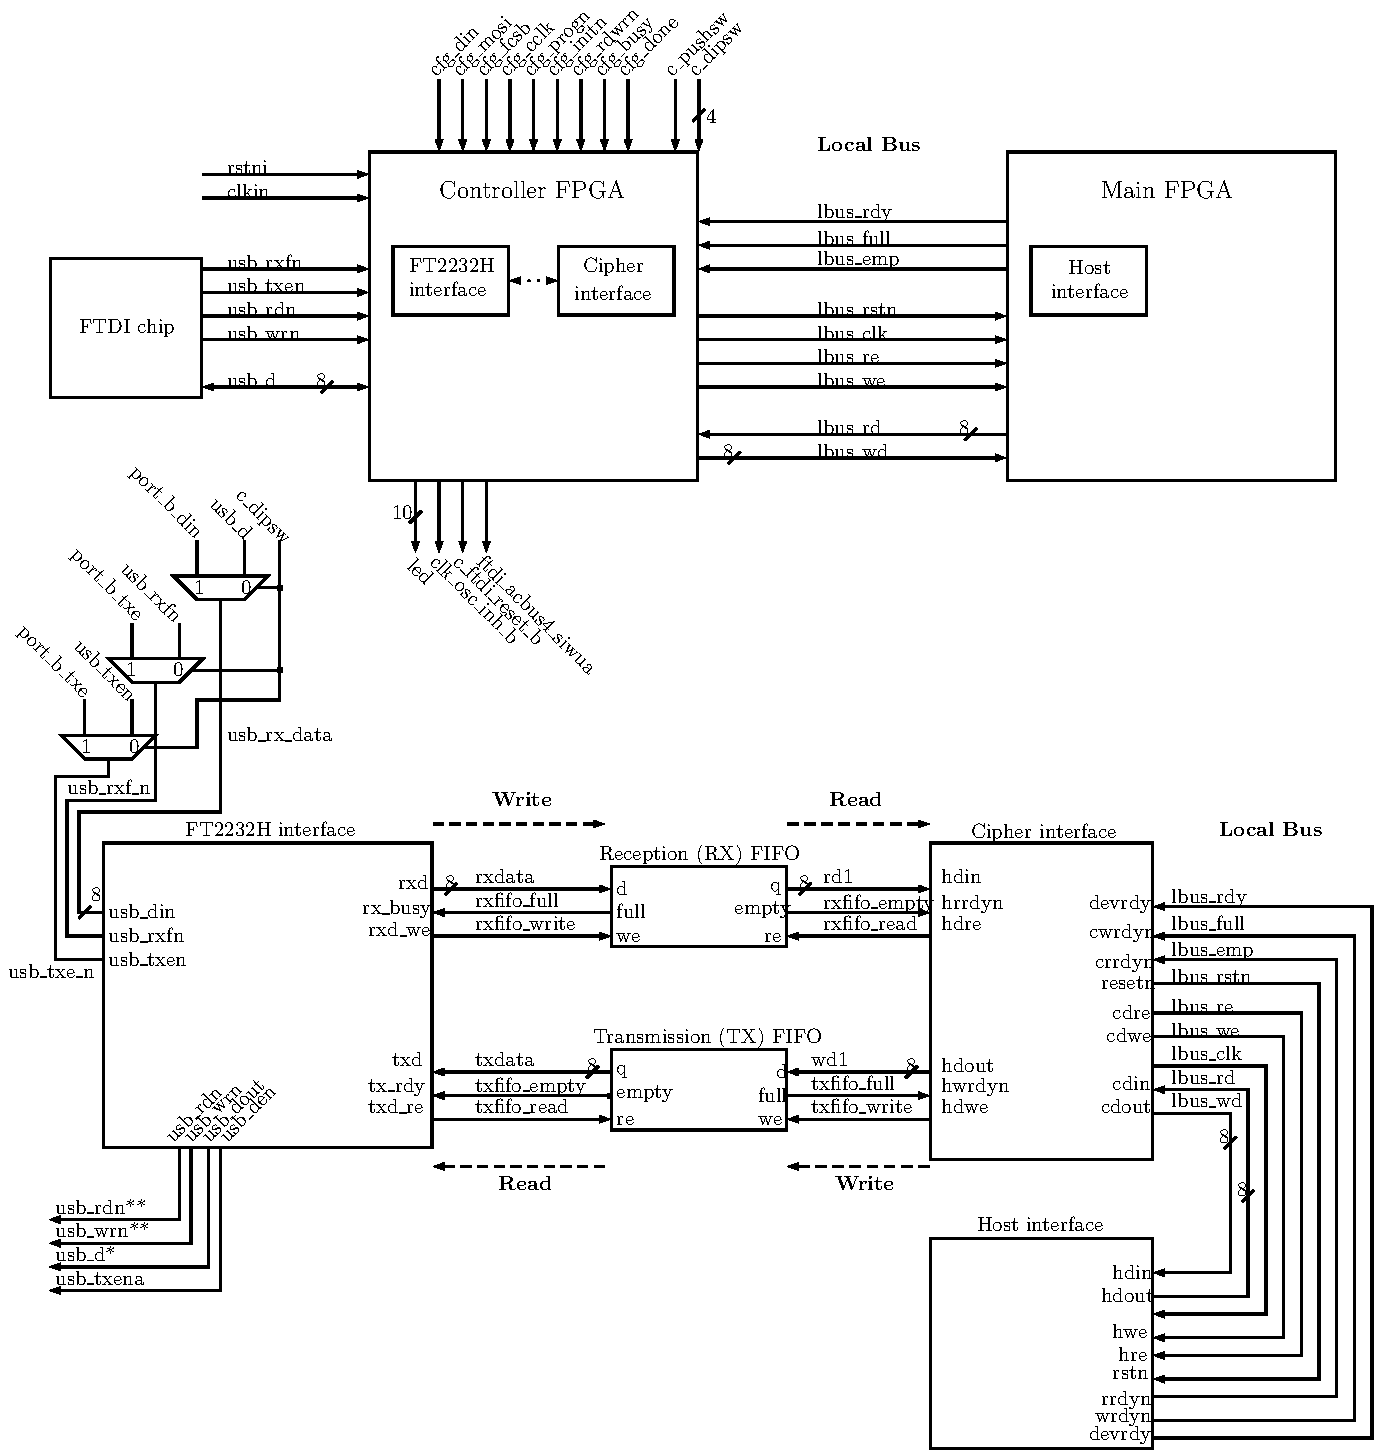
\includegraphics[scale=0.65]{sakura_g-signal-overview}
	\captionof{figure}{Overview of the interfaces used by both the main and control FPGAs. The control FPGA only moves data between the USB port and the control FPGA (via the FT2232H interface) and between the main FPGA and the control FPGA (via the Cipher interface).
	Data transmission between the Cipher interface and the FT2232H interface is done by making use of two FIFOs: a transmission (TX) and a reception (RX) FIFO. 
	The TX FIFO is used to transport data (written by the) Cipher interface to the FT2232H interface,
	while the RX FIFO is used to transport data from the FT2232H interface to the Cipher interface.
	Note that not all input signals are shown (e.g. the clock and reset signals for both FIFOs are omitted).
	The meaning of the single and double stars in some of the output signals from the FT2232H interface are as follows:\\
	%
	\textbf{*}: The value of \mintinline{text}{usb_d} contains the value that is read from the TX FIFO if the first bit of the DIP switch is low (i.e. \mintinline{text}{c_dipsw(0) = '0'})  (and when \mintinline{text}{usb_txena = '1'}). \\
	\textbf{**}: The value of \mintinline{text}{usb_rdn (usb_wrn)} equals the internal \mintinline{text}{usb_rdn (usb_wrn)} signal when the first bit of the DIP switch is low (i.e. \mintinline{text}{c_dipsw(0) = '0'}), otherwise it is a constant value of 1.
	}
	\label{fig: sakura_g-signal-overview}
\end{figure}
%
\begin{figure}
	\centering
	% !TeX spellcheck = en_US

\begin{tikzpicture}[->, >=stealth',shorten >=1pt,auto,node distance=2cm]
\node[state, initial] (idle) {$i$};

\node[state, above right of = idle] (read1) {$r_1$};
\node[state, right of = read1] (read2) {$r_2$};
\node[state, right of = read2] (read3) {$r_3$};

\node[state, below right of = read3] (back off) {$b$};

\node[state, below right of = idle] (write1) {$w_1$};
\node[state, right of = write1] (write2) {$w_2$};
\node[state, right of = write2] (write3) {$w_3$};

\draw (idle) edge[bend left, above] node[align=left, xshift=-40pt]{\mintinline{text}{usb_rxf_reg = '1'} \\ \mintinline{text}{rx_busy = '0'}} (read1);

\draw (idle) edge[bend right, below] node[align=left, xshift=-40pt, yshift=-10]{\mintinline{text}{usb_txe_reg = '1'} \\ \mintinline{text}{tx_rdy = '0'}} (write1);

\draw (read1) edge node{} (read2);
\draw (read2) edge node{} (read3);
\draw (read3) edge[bend left, below] node{} (back off);

\draw (back off) edge node{} (idle);

\draw (write1) edge node{} (write2);
\draw (write2) edge node{} (write3);
\draw (write3) edge[bend right, below] node{} (back off);

\draw (idle) edge [loop above, left, in=-30, out=30, looseness=5] (idle);
\end{tikzpicture}

	\captionof{figure}{Finite state machine used by the FT2232H interface to control the reading and writing from the FTDI USB chip. In the read states ($r_1, r_2, r_3$), a single byte is received from the USB channel in order to be sent to the main FPGA. In the write states ($w_1, w_2, w_3$), a single byte is transmitted over the USB channel.}
	\label{fig: usb_fsm}
\end{figure}
%
We give a short description for each of the interfaces:
%
\begin{itemize}
	\item \textbf{FT2232H interface}: this component reads data from the USB port (FTDI based) and writes in the internal reception FIFO (RX). 
	In addition, it also reads the transmission FIFO (TX) and sends it to the USB port (\Cref{fig: sakura_g-signal-overview}).
	Reading and writing from the FTDI chip is controlled by a finite state machine (FSM) (\Cref{fig: usb_fsm}).  
	This FSM starts in the idle state $(i)$, in which it is determined whether it can start to read data from the USB channel ($r_1$), write data to the USB channel ($w_1$) or remain in the idle state $(i)$. 
	We describe the read and write states in more detail:
	%
	\begin{itemize}
		\item \textbf{Read}. 
		If the RX FIFO is ready and not busy (\mintinline{text}{usb_rxf_reg = '1'} and \mintinline{text}{rx_busy = '0'} respectively), we proceed to the first read state ($r_1$). 
		Once we are in the second read state $(r_2)$, we read the actual byte from the USB channel, and set the write enable of the RX FIFO and indicate that this register is read ready. 
		Finally we proceed to the final read state $(r_3)$, in which the data read from the USB channel is actually written into the RX FIFO. 
		After resetting the write enable of the RX FIFO, we proceed to the back-off state $(b)$.
		
		\item \textbf{Write}.
		If the TX FIFO is ready (\mintinline{text}{usb_txe_reg = '1'} and \mintinline{text}{tx_rdy = '1'}), we proceed to the first write state $(w_1)$.
		In the first write state $(w_1)$, we reset the read enable of the TX FIFO and enable the output of the USB data bus. 
		In the second write state $(w_2)$, we indicate that the value from the TX FIFO is ready to be written to the USB port. 
		
		\item \textbf{Back off}.
		In the back off state $(b)$, we reset the USB write enable (which is low active).
		This signal is passed to the FTDI chip, which then knows that it can set the corresponding signals to send another byte.
		In addition, we also reset the output-enable signal (which indicates whether the output data is valid or not).
		
	\end{itemize}
	%
	\item \textbf{Cipher interface}: This is the interface with the main FPGA. This component controls the local bus between the control and the main FPGA.
	It reads the reception FIFO (RX) that the FT2232H interface writes, and writes content received from the local bus (i.e. written by the host interface) into the transmission (TX) FIFO (see \Cref{fig: sakura_g-signal-overview}).
	Reading and writing from the main FPGA (i.e. the host interface) is controlled by two state machines: 
	%
	\begin{figure}
		\centering
		\subfloat[Finite state machine used by the cipher interface to control the reading from the data written on the local bus by the host interface (i.e. main FPGA).]{
			% !TeX spellcheck = en_US

\begin{tikzpicture}[->, >=stealth',shorten >=1pt,auto,node distance=3cm]
\node[state, initial] (idle) {$i$};

\node[state, right of = idle] (read) {$r$};

\draw (idle) edge[bend left, above] node[align=left]{\mintinline{text}{devrdy = '1'} \\ \mintinline{text}{hwrrdyn = '0'} \\ \mintinline{text}{crrdyn = '0'}} (read);

\draw (idle) edge [loop above, left, out=-60, in=-120, looseness=5] (idle);

\draw (read) edge [bend left, below] (idle);

\end{tikzpicture}

			\label{subfig: cipher read fsm}
		}
		\hspace{0.5cm}
		\subfloat[Finite state machine used by the cipher interface to control the writing to the local bus connected to the main FPGA.]{
			% !TeX spellcheck = en_US

\begin{tikzpicture}[->, >=stealth',shorten >=1pt,auto,node distance=3cm]
\node[state, initial] (idle) {$i$};

\node[state, right of = idle] (fifo read) {$r$};

\node[state, right of = fifo read] (lbus write) {$w$};

%\draw (idle) edge[bend left, above] node[align=left]{\mintinline{text}{hwrdyn = '0'} \\ \mintinline{text}{crrdyn = '0'}} (read);

\draw (idle) edge [loop above, left, out=-60, in=-120, looseness=5] (idle);
\draw (idle) edge node[align=left, yshift = 15] {\mintinline{text}{hwrdyn = '0'} \\ \mintinline{text}{crrdyn = '0'}} (fifo read);
\draw (fifo read) edge (lbus write);
\draw (lbus write) edge[loop above, left, out=120, in=60, looseness=5] node[xshift=30, yshift=10] {\mintinline{text}{cwrdyn = '1'}} (lbus write);
\draw (lbus write) edge [bend left, below] node[align=left]{\mintinline{text}{cwrdyn = '0'}} (idle);

\end{tikzpicture}

			\label{subfig: cipher write fsm}
		}			
		\captionof{figure}{State machines used by the cipher interface to control the reading from and writing to the host Interface.}
		\label{fig: cipher_rw_fsm}
	\end{figure}
	%
	\begin{itemize}
		\item \textbf{Cipher Read} (\Cref{subfig: cipher read fsm}): This state machine controls the reading from data that is written on the local bus by the host interface. The FSM starts in the idle state ($i$), in which it waits until the main FPGA is ready, the host interface is write ready and the cipher interface is read ready (see \Cref{subfig: cipher read fsm}). If this is the case, the FSM moves to the read state $(r)$. In addition, it sets the read enable and clears the write enable of the host. In the read state, the input received over the local bus (\mintinline{text}{lbus_rd}) is written to the TX FIFO. The values of the cipher read and host write enable are restored to their original values.		
			
		\item \textbf{Cipher Write} (\Cref{subfig: cipher write fsm}): This state machine controls the writing on the local bus, which is read by the host interface. The FSM starts in the idle state $(i)$, in which it waits until the host interface is write ready, and the cipher interface is read ready. If this is the case, the FSM moves to a read state in which it reads data from the Reception (RX) FIFO. In the write state, this data is then transmitted over the local bus such that it can be read by the host interface.
	\end{itemize}
	%
	\item \textbf{Host interface}: This component reads and writes the local bus between the control and the main FPGA. It is mainly a state machine. It controls the implementation through the values that are written in the bus. 
	Received values are stored in registers.
	Depending on the received value and the appropriated control signals (e.g. write enable (WE)), parts of the register are assigned specific values.
	This component consists of two registers: \mintinline{shell}{addr_reg} and \mintinline{shell}{data_reg}. 
\end{itemize}
%
% !TeX spellcheck = en_US
% !TeX root = ../Tom_Sandmann-master_thesis

\section{IP blocks} \label{sec: IP Blocks}
The hardware design of {\fourq} \cite{jarvinen2016four} (\Cref{chp: FourQ On Hardware}) makes use of a couple of Intellectual Property (IP) blocks provided by Xillinx.
An IP block is a reusable unit of logic, which is the intellectual property of one party.
The IP blocks, and their corresponding configurations, used within the {\fourq} hardware design are as follows:
%
\begin{itemize}
	\item \textbf{\mintinline{text}{blk_mem_gen_0}}: \\ Memories \& Storage Elements $\to$ RAMs \& ROMs \& BRAMs $\to$ Block Memory Generator
	\begin{table}[H]
		\centering
		\begin{tabular}{cc}
			\toprule
			\textbf{Setting} & \textbf{Value} \\
			\midrule
			Memory type & True Dual-Port RAM \\
			Clocking Options & Common Clock \\
			Port A/B Write Width & 128 \\
			Port A/B Write Depth & 256 \\
			Port A/B Enable & Use ENA/ENB Pin \\
			Port A/B & Register Port A/B output of Memory Primitives \\
			All other options & Keep defaults \\
			\bottomrule
		\end{tabular}
	\end{table}
	%
	\item \textbf{\mintinline{text}{blk_mem_gen_1}}: \\ Memories \& Storage Elements $\to$ RAMs \& ROMs \& BRAMs $\to$ Block Memory Generator
	\begin{table}[H]
		\centering
		\begin{tabular}{cc}
			\toprule
			\textbf{Setting} & \textbf{Value} \\
			\midrule
			Memory type &  Single Port ROM\\
			Algorithm & Fixed Primitives $\to$ Primitive (Write Port A): 1kx18 \\
			Port A Write Width & 25 \\
			Port A Write Depth & 8192 \\
			Port A Enable & Use ENA Pin\\
			Port A & Register Port A output of Memory Primitives \\
			Load Init file & \mintinline{text}{prog_code.coe} \\
			All other options & Keep defaults \\
			\bottomrule
		\end{tabular}
	\end{table}
	%
	\item \textbf{\mintinline{text}{mult_gen_0}}: \\ Math Functions $\to$ Multipliers $\to$ Multiplier
	\begin{table}[H]
		\centering
		\begin{tabular}{cc}
			\toprule
			\textbf{Setting} & \textbf{Value} \\
			\midrule
			Port A/B data type & Unsigned \\
			Port A/B width & 64 \\
			Multiplier Construction & Use Mults \\
			Pipeline stages & 7 \\
			All other options & Keep defaults \\
			\bottomrule
		\end{tabular}
	\end{table}
	%
\end{itemize}
%

% !TeX spellcheck = en_US
% !TeX root = ../Tom_Sandmann-master_thesis
\section{Reading and writing of internal registers}
The hardware design of {\fourq} requires us to first load specific constants into the RAM.
These constants are used during the scalar multiplication, and reduce the number of computations necessary.
In \Cref{chp: FourQ}, we describe these constants in more detail.
After the constants are loaded into RAM, the design can be controlled by specific operations.
These operations are described in \Cref{subsec: Control Logic}.
To control data assignment to the RAM, we make use of a FSM at the main FPGA.
This FSM can be seen in \Cref{fig: host fsm}.
%
\begin{figure}
	\centering
	% !TeX spellcheck = en_US

\begin{tikzpicture}[->, >=stealth',shorten >=1pt,auto,node distance=2cm]
\node[state, initial] (cmd) {$i$};
\draw (cmd) edge [loop above, left, in=60, out=120, looseness=5] (cmd);

\node[state, right of = cmd] (write addr msb) {$w_1$};
\node[state, right of = write addr msb] (write addr lsb) {$w_2$};
\node[state, right of = write addr lsb ] (write data msb) {$w_3$};
\node[state, right of = write data msb ] (write data lsb) {$w_4$};

\node[state, below of = write addr lsb] (wait read effective) {$r_{wait}$};
\node[state, right of = wait read effective] (read data msb) {$r_3$};
\node[state, right of = read data msb ] (read data lsb) {$r_4$};


\draw (cmd) edge node{} (write addr msb);
\draw (write addr msb) edge node{} (write addr lsb);
\draw (write addr lsb) edge node{} (wait read effective);
\draw (wait read effective) edge [loop above, left, in=150, out=210, looseness=5] (wait read effective);
\draw (wait read effective) edge node{} (read data msb);
\draw (read data msb) edge node{} (read data lsb);

\draw (write addr lsb) edge node{} (write data msb);
\draw (write data msb) edge node{} (write data lsb);

\draw (write data lsb) edge [bend right, above] node{} (cmd);

\draw (read data lsb) edge [bend left=50] node{} (cmd);

\end{tikzpicture}

	\captionof{figure}{Finite state machine used by the host interface to control the reading from and writing to the internal registers and control signals of the {\fourq} component.}
	\label{fig: host fsm}
\end{figure}
%
The FMS writes the \mintinline{text}{data_reg} and \mintinline{text}{addr_reg} values. 
Based on the values in these registers, the {\fourq} input signals are controlled.
We describe the FSM of \Cref{fig: host fsm} in more detail.
In both the reading and writing states, first the value of the address is transmitted  $(w_1, w_2)$ followed by a data read/write ($(r_3, r_4)$ or $(w_3, w_4)$ respectively).
Because values of both the address and data are 2 bytes, and we can only transmit one byte at a time, this transmission is done in two steps: the most significant byte (MSB) is sent first, followed by the least significant byte (LSB).
If the FSM is in the reading state and the address value has been transmitted, the address value is used to determine the output of the host interface.
This is realized by a multiplexer, where the value of the address determines which output signals are retrieved.
In the final design, reading from the main FPGA is primary used to retrieve the \texttt{busy} control signal, or (parts of) the result point of the scalar multiplication. 
The multiplexer can also be used to verify whether data assignments are done correctly within the interface itself.

The reason for the address to be 2 bytes is due to the size of the addresses within {\fourq} to load the RAM constants.
These addresses are 9 bits, where the first bit indicates whether we write the lower or upper half of the 128-bits value.
The remaining 8 bits specify the value of the address.
Fortunately, these data and address sizes are also used in the example main FPGA design that comes with the SAKURA-G, and required (almost) no change.

If we want to write data values to the main FPGA, the address is used by the hardware design to control the assignment of data (which are transmitted after the address) to the correct range of a signal.
Once the address is transferred, 2 bytes of data are transmitted.
After this is done, a control signal indicates that the assignment of data to the address can be made. 
If the address is not known internally, all values keep their previous value.
In the case of reading, there is an additional state in the FSM which waits for the value-to-read to become available.
The reason for this is due to a read latency of five periods.
The first three periods in this latency are because of how the interface of the memory is done in the {\fourq} design.
The remaining two periods are due to the two pipeline stages when reading from the True Dual-Port RAM (TDPR).
In general, the latency for either of the ports of the TDPR can be seen in the corresponding Block Memory Generator (BMG) configuration (see \Cref{sec: Interface with the board}).

% !TeX spellcheck = en_US
% !TeX root = ../Tom_Sandmann-master_thesis
\section{Capturing power traces}
To perform side channel analysis of the {\fourq} hardware design on the FPGA, we need to obtain power traces as {\fourq} is calculating the scalar multiplication.
A power trace is a collection of samples.
Each sample is a tuple of voltage and time values.
Time values are represented in seconds (s), while the amplitude values are represented in volts (v).
To obtain power traces, the FPGA is connected to the oscilloscope.
The SAKURA-G is designed with ultra-low noise in mind.
The board provides a couple of SMA connectors that can be used to monitor the power waveforms. 
The board also comes with an on-board amplifier, which can used to monitor the amplified waveform (for both the control and main FPGAs).
To control the acquisition of a power trace, we make use of a trigger.
The trigger tells the oscilloscope when it should start the acquisition of a waveform (i.e. when the value of the trigger is high) and when this acquisition should stop (i.e. when the oscilloscope's memory is full). 
The oscilloscope used to display and retrieve the captured power traces is the Teledyne LeCroy - WaveRunner 610Zi.
To connect with the oscilloscope and retrieve the acquired waveforms, an Ethernet cable (ENET) was employed.
Teledyne LeCroy oscilloscopes employ a standard Ethernet interface for utilizing the TCP/IP transport layer \cite{automation2017manual}.
Other methods for making the remote connection exist as well (such as USBTMC, GPIB and LSIB).
To interface with the oscilloscope, we make use of ActiveDSO, which is an ActiveX control.
ActiveDSO provides interface drivers and a client library to make the remote connection over ENET, GPIB or USBTMC interfaces.
It also supports many automation features besides remote control. One can read more about how Teledyne LeCroy oscilloscopes can be controlled by a variety of Windows applications and programming languages in the ActiveDSO's developer guide \cite{activedso2015guide}.
As the interface with the SAKURA-G board is written in Python, this is also the language of choice for communicating with the oscilloscope.
In Python, the control object used to communicate with the oscilloscope is instantiated as follows:
%
\begin{minted}[xleftmargin=\parindent, tabsize=4, obeytabs, breaklines, fontsize=\footnotesize]{python3}
command = "LeCroy.ActiveDSOCtrl.1"
_scope = win32com.client.Dispatch(command)
\end{minted}
%
Using the control object, we can write commands to the oscilloscope and read back the response. To make this possible, we connect to the oscilloscope:
%
\begin{minted}[xleftmargin=\parindent, tabsize=4, obeytabs, breaklines, fontsize=\footnotesize]{python3}
ip_address="192.168.0.1"
command = "IP:" + ip_address
_scope.MakeConnection(command)
\end{minted}
%
The IP address should match the IP address set in the settings of the oscilloscope.
After establishing a connection with the oscilloscope, we can use the control object to send commands to the device.
ActiveDSO supports two types of commands that can be sent to the oscilloscope using the instantiated control.
Both traditional IEEE 488.2 (GPIB) commands and the Windows\textsuperscript{\textregistered} Component Object Model (COM) commands can be used.
Examples of these commands are as follows:
%
\begin{minted}[xleftmargin=\parindent, tabsize=4, obeytabs, breaklines, fontsize=\footnotesize]{python3}
# 488.2 format
scope.WriteString("<command string>", <Boolean EOI>)
# Automation Control within the VBS command
scope.WriteString("app.Shutdown", True)
\end{minted}
%
If End of Identify (EOI) is set to 1 (\mintinline{text}{True}), the command terminates with EOI, and the device interprets the command right away. This is normally the desired behavior.
If EOI is set to 0 (\mintinline{text}{False}), a command may be sent in several parts with the device starting to interpret the command only when it receives the final part.
This final command should have set its EOI value set to (\mintinline{text}{True}).
If a command string contains characters like double quotes ("), the command string should be surrounded with triple quotes.
Otherwise, Python would interpret the first double quote as the end of the command string, which is unintended.

The oscilloscope offers a variety of interfaces for using devices to input analog or digital signals. 
A series of connectors arranged on the front of the instrument are used to input analog signals on channels 1-4. 
We use these analog inputs to connect our FPGA to the oscilloscope. 
Each of these channels interfaces power probes and completely integrates the probe with the channel. 
When connected, the probe type is recognized and some setup information, such as input coupling and attenuation, is performed automatically.
Besides these analog inputs, one can also make use of probes and the LBUS interface.
In our setup, we only use the analog inputs to capture the power traces of our FPGA.
To get the waveform from a corresponding channel, we have to call the appropriate ActiveDSO method.
The available methods for acquiring a waveform can be seen in \cite{activedso2015guide}.
%
%\begin{itemize}
%	\item \texttt{GetByteWaveform}. This method reads raw 8-bit waveform data from the instrument into a byte array. Visual Basic's (unsigned) byte type (values between 0 and 255) is used to store the signed data bytes (values between -128 and 127) that the scope emits. 
%	To make this work, the signed data is `shifted' by 128, such that it can fit in the unsigned data type. 
%	This should be remembered when the data is scaled.
%	The \texttt{GetByteWaveform} method should be used when unscaled 8-bit waveform data is required. 
%	Processed waveforms are usually 16-bit waveforms. 
%	To avoid losing precision, they should be transmitted in 16 bit form. 
%	This can be done by making use of the \texttt{GetIntegerWaveform} method.
%	
%	\item \texttt{GetIntegerWaveform}. This method reads raw 16-bit waveform data from the instrument into an integer array. 
%	This method should be used when unscaled 16-bit waveform data is required. 	
%	Processed waveforms are usually 16-bit waveforms. 
%	To avoid losing precision, they should be transmitted in 16-bit format.
%	Channel waveforms are usually 8-bit waveforms. 
%	They may be transferred using the \texttt{GetByteWaveform} method. 
%	This reduces the time and storage requirements.
%	
%	\item \texttt{GetNativeWaveform}. This methods reads a waveform from the instrument in its native binary form. 
%	You can specify whether the data should be transmitted as 16-bit words or as regular 8-bit bytes.
%	A parameter for this method is also used to specify which entity of the waveform should be transmitted.
%	Possible values fort his parameter are the descriptor (DESC), the user text (TEXT), the time descriptor (TIME), the data block (DAT1), a second block of data (DAT2) or all entities (ALL).
%	As mentioned in the previous described methods, processed waveforms are usually 16-bit waveforms and should be captured by setting the word data argument to \mintinline{text}{True}.
%	Channel waveforms ($C_1, \ldots, C_4$) should be transmitted by setting the word data argument to \mintinline{text}{False}.
%	It is also possible to restore a waveform captured using the \texttt{GetNativeWaveform}.
%	This is only possible if the waveform was captured using the (ALL) parameter.
%	If this is the case, the \texttt{SetNativeWaveformSetNativeWaveform} can be used to restore the waveform.
%	
%	\item \texttt{GetScaledWaveform}. This method reads a scaled waveform from the instrument. 
%	The result is a scaled waveform stored as an array of single-precision floating point values.
%	If the time value corresponding to each sample amplitude is required, the \texttt{GetScaledWaveformWithTimes} method should be used.
%	
%	\item \texttt{GetScaledWaveformWithTimes}. This method reads a scaled waveform from the instrument and stores the time and amplitude at each sample point.
%	The result is a scaled waveform stored as a two-dimensional array of single-precision floating point values. In the first column, the time values are stored. In the second column, the amplitude values are stored.
%	If the time value corresponding to each sample amplitude is not required, one can use the \texttt{GetScaledWaveform} method.
%	
%\end{itemize}
%%

%If 16-bit words are send from the oscilloscope, we have to take the order in which the bytes for a single word are stored into account.
%To determine which byte order the oscilloscope is currently using waveform data transmission, we can make use of the \mintinline{text}{COMM_ORDER} command. 
%This command can be used to either ask for the current communication order or to set the communication order.
%When setting the communication order using the \mintinline{text}{COMM_ORDER} command, we use the following command syntax: \mintinline{text}{COMM_ORDER <mode>}, with \mintinline{text}{<mode> := {HI, LO}}.
%If \mintinline{text}{HI} is used, waveform data is sent with the most significant byte (MSB) first (i.e. big endian). 
%If \mintinline{text}{LO} is used, waveform data is sent with the least significant byte (LSB) (i.e. little endian).
%As we can read in the Remote Control Manual, data should be sent with the LSB first for Intel-based computers.
%For Motorola-based computers, data should be sent with the MSB first, the default at power-up. Data written to the instrument's hard disk, USB, or floppy always remains in LSB first format (the default DOS format). You cannot use the \mintinline{shell}{COMM_ORDER} command in these cases, since it is only meant for data sent using GPIB and RS-232-C ports.
%
%Before acquiring a waveform using these methods, we can specify some additional information about the transfer of these waveform. 
%This is done by making use of the \texttt{SetupWaveformTransfer}.
%This method is used to configure various parameters that control the transfer of waveforms from the instrument to the PC.
%These arguments are as follows:
%%
%\begin{itemize}
%	\item \mintinline{text}{first_point}: An integer that describes the first point to transfer. A value of 0 indicates the first point.
%	
%	\item \mintinline{text}{sparsing}: An integer that describes the sparsing factor. This value indicate which values in the sample should be skipped.
%	A value of 0 indicates that all points should be transfered, while a value 2 means that every other point should be skipped.
%	
%	\item \mintinline{text}{segment_no}: An integer that specifies which segment number to transfer. A value of 0 indicates that all segments should be transferred.
%\end{itemize}
%%
%For the majority of these cases, the default values for these settings will be sufficient. This means that: all points are transferred, starting from the first point and transferring all segments.


















	% !TeX spellcheck = en_US
% !TeX root = ../Tom_Sandmann-master_thesis
\chapter{Elliptic Curves} \label{chp: Elliptic Curves}
\lettrine[lhang = 0.4, findent=-30pt, lines=4]{\textbf{
		\initfamily \fontsize{20mm}{20mm} \selectfont I
		\normalfont}}{n} 
this chapter, we discuss the basics of elliptic curves.
We specifically take a look at (twisted) Edwards curves, operations on points on these curves and alternative point representations for these curves.
Alternative representations provide faster point addition and doubling.
Multiple of such efficient representations are used internally in {\fourq} (see \Cref{chp: FourQ}).
For more information on finite fields, we refer to the excellent section on finite fields with respect to AES in \cite[§4.3]{paar2009understanding}.

% !TeX spellcheck = en_US
% !TeX root = ../Tom_Sandmann-master_thesis
\section{Definition}
An elliptic curve $E$ over a field $K$ in long Weierstrass form is given by the following equation \cite{peter2008elliptic}:
%
\begin{align*}
E: y^2 + a_1 xy + a_3y = x^3 + a_2 x^2 + a_4x + a_6
\end{align*}
%
with $a_i \in K$ for $i \in \{1,\ldots,6\}$.
To avoid singularities on the curve, it is necessary that both partial derivatives do not vanish simultaneously for each point $(x,y)$ over $\bar{K}$%
\footnote{$\bar{K}$ denotes the algebraic closure of the field $K$}.
%
These partial derivatives are given as follows:
%
\begin{align*}
\pdv{K}{y} &= 2y + a_1 x + a_3, ~~~~~~~ \pdv{K}{x} = 3x^2 + 2a_2x + a_4 - a_1 y
\end{align*}
%
If the characteristic of the coefficient field is not equal to 2 or 3 ($\operatorname{char}(k) \neq 2,3$), we can transform the curve to short Weierstrass form. This short Weierstrass form is given as follows:
%
\begin{align*}
E_{a, b}: y^2 = x^3 + ax + b
\end{align*}
%
where $a,b \in K$. 
The definition of an elliptic curve requires the curve to be non-singular. 
This means that it does not have cusps, self-intersections or isolated points. 
This non-singularity property is satisfied if and only if the discriminant of $E$ is unequal to zero:
%
\begin{align*}
\triangle = -16(4a^3 + 27b^2) \neq 0
\end{align*}
%
All the points on $E$ together with the imaginary point at infinity $\mathcal{O}$ form an additive group $(E, \oplus)$ \cite{peter2008elliptic}:
%
\begin{itemize}
	\item The neutral element in this group is $\mathcal{O}$;
	\item The inverse of a point $P=(x,y)$ is defined as $-P = (x, -y)$, with $P + (-P) = \mathcal{O}$;
	\item Given two points $P=(x_1, y_1)$ and $Q = (x_2, y_2)$, we have $P \oplus Q = (x_3, y_3)$ where:
	%
	\begin{align*}
	x_3 &= s^2 - x_1 - x_2 \\
	y_3 &= s(x_1 - x_3) - y_1
	\end{align*}
	%
	with
	%
	\begin{align*}
	s &= 	\begin{cases}
				\frac{y_2 - y_1}{x_2 - x_1} 	& \text{if $P \neq \pm Q$ (point addition) }\\
				\frac{3 x_1^2 + a}{2y_1}		& \text{if $P = Q$ (point doubling)}
			\end{cases}	
	\end{align*}
	%
\end{itemize}
%
If we consider a curve that is defined over the real numbers, we have a nice geometric interpretation of the addition, doubling and inversion operations.
These interpretations can be seen in \Cref{fig: elliptic curve operations geometric interpretation}.
%
\begin{figure}
	\centering
	\subfloat[Addition of a point on an elliptic curve over the real numbers.]{
	\begin{tikzpicture}
    \begin{axis}[
        xmin=-3,
        xmax=4,
        ymin=-7,
        ymax=7,
        xlabel={$x$},
        ylabel={$y$},
        scale only axis,
        axis lines=middle,
        % set the minimum value to the minimum x value
        domain=-2.456678:4,      % <-- works for pdfLaTeX and LuaLaTeX
        samples=1000,
        smooth,
        % to avoid that the "plot node" is clipped (partially)
        clip=false,
        % use same unit vectors on the axis
        axis equal image=true,
        xticklabels={,,},
        yticklabels={,,}
    ]
        \addplot [black] {sqrt(x^3-4*x+5)};
        \addplot [black] {-sqrt(x^3 - 4*x + 5)};
        
         % Some math constant macros
         \pgfmathsetmacro\localmaximum{-2/sqrt(3)}
        
       	% add nodes to the points and the corresponding labels
       	\node [label={$P$}, circle,fill,inner sep=1.5pt] (P) at (\localmaximum, 2.842) {};
       	\node [label=below:{$Q$}, circle,fill,inner sep=1.5pt] (Q) at (-\localmaximum, -1.368) {};
       	% draw a line from (P) a bit further than just to (Q)
       	\draw [black] ($ (Q)!1.5!(P) $) --  (P) -- ($ (P)!2.5!(Q) $);
       	% Specify node at intersection point
       	\node [above,circle,fill,inner sep=1.5pt] (I) at (3.31185, -5.29888 - 0.1) {};
       	% Specify result node
       	\node [label=right:{$P + Q$},above,circle,fill,inner sep=1.5pt] (R) at (3.31185, 5.29888) {};
       	% Draw line
       	\draw [black, dashed] (I) -- (R);
       	 
    \end{axis}
\end{tikzpicture}
	\label{subfig: elliptic_curve_add}
	}
	\hspace{0.5cm}
	\subfloat[Doubling of a point on an elliptic curve over the real numbers.]{
	\begin{tikzpicture}
    \begin{axis}[
        xmin=-3,
        xmax=4,
        ymin=-7,
        ymax=7,
        xlabel={$x$},
        ylabel={$y$},
        scale only axis,
        axis lines=middle,
        % set the minimum value to the minimum x value
        domain=-2.456678:4,      % <-- works for pdfLaTeX and LuaLaTeX
        samples=1000,
        smooth,
        % to avoid that the "plot node" is clipped (partially)
        clip=false,
        % use same unit vectors on the axis
        axis equal image=true,
        xticklabels={,,},
        yticklabels={,,}
    ]
        \addplot [black] {sqrt(x^3-4*x+5)};
        \addplot [black] {-sqrt(x^3 - 4*x + 5)};
        
         % Some math constant macros
        \pgfmathsetmacro\localmaximum{-2/sqrt(3)}
        \pgfmathsetmacro\xcoordinateintersection{4/sqrt(3)}
        \pgfmathsetmacro\ycoordinateintersection{sqrt(5 + 16/(3 * sqrt(3)))}
        
       	% add nodes to the points and the corresponding labels
       	\node [label={$P$}, circle,fill,inner sep=1.5pt] (P) at (\localmaximum, 2.842) {};
       	% Specify node at intersection point
       	\node (I) [above,circle,fill,inner sep=1.5pt] at (\xcoordinateintersection, \ycoordinateintersection) {};
       	% draw a line from (P) a bit further than just to (I)
       	\draw [black] ($ (I)!1.5!(P) $) --  (P) -- ($ (P)!1.5!(I) $);
       	% Specify result node
       	\node [label=below:{$2P$}, circle,fill,inner sep=1.5pt] (R) at (\xcoordinateintersection, -\ycoordinateintersection) {};
       	% Draw line
       	\draw [black, dashed] (I) -- (R);
    \end{axis}
\end{tikzpicture}
	\label{subfig: elliptic_curve_dbl}
	}
	\hspace{0.5cm}
	\subfloat[Inversion of a point on an elliptic curve over the real numbers.]{
		\begin{tikzpicture}
    \begin{axis}[
        xmin=-3,
        xmax=4,
        ymin=-7,
        ymax=7,
        xlabel={$x$},
        ylabel={$y$},
        scale only axis,
        axis lines=middle,
        % set the minimum value to the minimum x value
        domain=-2.456678:4,      % <-- works for pdfLaTeX and LuaLaTeX
        samples=1000,
        smooth,
        % to avoid that the "plot node" is clipped (partially)
        clip=false,
        % use same unit vectors on the axis
        axis equal image=true,
        xticklabels={,,},
        yticklabels={,,}
    ]
        \addplot [black] {sqrt(x^3-4*x+5)};
        \addplot [black] {-sqrt(x^3 - 4*x + 5)};
        
         % Some math constant macros
        \pgfmathsetmacro\localmaximum{-2/sqrt(3)}       
       	% add nodes to the points and the corresponding labels
       	\node [label={$P$}, circle,fill,inner sep=1.5pt] (P) at (\localmaximum, 2.842) {};
		\node [label=below:{$-P$}, circle,fill,inner sep=1.5pt] (-P) at (\localmaximum, -2.842) {};
       	\draw [black, dashed] (-P) -- (P);
    \end{axis}
\end{tikzpicture}
		\label{subfig: elliptic_curve_inv}
	}
	\captionof{figure}{Geometric interpretation of point addition, doubling and inversion when considering an elliptic curve over the real numbers \cite{paar2009understanding}.}
	\label{fig: elliptic curve operations geometric interpretation}
\end{figure}
%
If we work with elliptic curves, it is important to know the order of the group.
This order plays a key role in the hardness of the discrete log problem (DLP) that can be constructed with elliptic curves.
Hasse's theorem states that the number of points of an elliptic curve modulo a prime $p$ is roughly in the range of the prime $p$.
Each point on the curve also has an order.
The order of a point $P$ is the smallest positive integer $n$ such that:
%
\begin{align*}
[n]P = \overbrace{P \oplus \ldots \oplus P}^{n \text{ times}} = \mathcal{O}
\end{align*}
%
Some points never add up to $\mathcal{O}$, which gives them an infinite order.
The order of the neutral element is 1.
In cryptography, elliptic curves are treated on a given finite field, for example $K = \mathbb{F}_{p}$, with $p$ being a sufficiently large prime number.
Points on an elliptic curve together with the neutral element $\mathcal{O}$ have cyclic subgroups.
To make all points on the elliptic curve form a cyclic group, certain conditions have to be met.
$K = \mathbb{F}_{p}$ with $p > 3$ must hold.
In addition, the discriminant of the curve has to be non-zero (as mentioned earlier).
There are also other mathematical properties leading to cryptographic weaknesses that need to be ruled out.
Due to the complexity of constructing save curves, we often make use of standardized curves in practice.
Because we know the basic math behind elliptic curves, we can now construct a DLP over these curves \cite{paar2009understanding}:
%
\begin{definition}[Elliptic Curve Discrete Logarithm Problem (ECDLP)]
Given an elliptic curve $E$, a primitive element (also called a generator) $P$ and another element $T$. 
The discrete logarithm problem is finding the integer $d$, with $1 \le d \le \#(E)$ (with $\#(E)$ being the number of points on the curve) such that:
%
\begin{align*}
\overbrace{P \oplus P \oplus \ldots \oplus P}^{d \text{ times}} = dP = T
\end{align*}
%
\end{definition}
%
In cryptosystems, the value of $d$ becomes the private key, while the public key is $T$, where $T=(x_t, y_t)$ is a point on the curve.

% !TeX spellcheck = en_US
% !TeX root = ../Tom_Sandmann-master_thesis
\section{Twisted Edwards curves} \label{sec: Twisted Edwards curves}
Edwards curves are a family of elliptic curves \cite{edwards2007normal}.
An Edwards curve over a field $K$ having a characteristic unequal to 2 is defined as follows:
%
\begin{align*}
x^2 + y^2 = 1 + dx^2 y^2
\end{align*}
%
with scalar $d \in K \setminus \{0, 1\}$.
A more general form which introduces additional parameters also belongs to this family of curves:
%
\begin{align*}
x^2 + y^2 = c^2(1 + dx^2 y^2)
\end{align*}
%
with $c, d \in K$ and $c \cdot d (1 - c^4 \cdot d) \neq 0$.
The value of $c$ however is often fixed at 1.
This is also assumed when we introduce the addition and subtraction formula's for Edwards curves.
Every Edwards curve is birationally equivalent to an elliptic curve in Weierstrass form.
% https://crypto.stackexchange.com/questions/43013/what-does-birational-equivalence-mean-in-a-cryptographic-context
When we have geometric objects like elliptic curves, we want to define what it means for these two objects to be ``the same''.
Given two curves $E_1$ and $E_2$, we say that they are ``the same'' when they are isomorphic. Given two mathematical objects, they are said to be isomorphic if there exists an isomorphism between them. An isomorphism is a structure-preserving map (also called a homomorphism) that has an inverse.
Besides this way of equating objects, we also have another way of equating them.
That is by stating they are ``almost the same''.
This is exactly what a birational equivalence can be used for.
Two curves $E_1$ and $E_2$ are birationally equivalent when there exists a map $\phi : E_1 \to E_2$ between the two curves which is defined at every point of $E_1$ except for a small subset.
In addition, there is also an inverse map $\phi^{-1} : E_2 \to E_1$ which is again defined at every point of $E_2$ except for a small subset.
% https://crypto.stackexchange.com/questions/27842/edwards-montgomery-ecc-with-weierstrass-implementation
Before we show the birational equivalence between an Edwards curves and an elliptic curve in Weierstrass form, we first introduce a generalization of Edwards curves, which are called twisted Edwards curves \cite{bern2008twisted}.
Each twisted Edwards curve is a twist of an Edwards curve.
If we have an elliptic curve $E$ over a field $K$, then there exists a so-called quadratic twist, which is another elliptic curve which is isomorphic to $E$ (over an algebraic closure of $K$).
Given a field $K$ with $\operatorname{char}(k) \neq 2$, we define a twisted Edwards curve with the following equation:
%
\begin{align*}
E_{E,a,d} : ax^2 + y^2 = 1 + dx^2y^2
\end{align*}
%
with $a,d \in K \setminus \{0\}$ and $a \neq b$.
Note that a `normal' Edwards curve is just a specific instance of a twisted Edwards curve (it fixes $a = 1$). 
It can be shown that every twisted Edwards curve is birationally equivalent to an elliptic curve in Montgomery form and vice versa \cite{bern2008twisted}.
In addition, every Montgomery curve is also birationally equivalent to an elliptic curve in Weierstrass form.
A Montgomery curve is also a form of an elliptic curve. 
A Montgomery curve over a field $K$ is defined as follows:
%
\begin{align*}
E_{M, A, B} : Bv^2 = u^3 + Au^2 + u
\end{align*}
%
with $A, B \in K$ and $B(A^2 - 4) \neq 4$.
As with the curves we have described previously, this curve is generally considered over a finite field $K$ with characteristic unequal to 2 and $A \in K \setminus \{-2, 2\}$ and $B \in K \setminus \{0\}$.
The corresponding birational maps between these three curves are defined as follows \cite{bern2008twisted}:
%
\begin{theorem}[Birational equivalence between Montgomery curves and twisted Edwards curves]
	Let $E_{E,a,d}$ and $E_{M,A, B}$ be elliptic curves in twisted Edwards form and Montgomery form respectively (with their corresponding definitions as introduced earlier).
	A twisted Edwards curve $E_{E,a,d}$ is birationally equivalent to the Montgomery curve $E_{M, A, B}$, where:
	%
	\begin{align*}
		A = \frac{2(a + d)}{(a - d)} \text{, and } B = \frac{4}{a - d}
	\end{align*}
	%
	The birational equivalence from $E_{E_{a,d}}$ to $E_{M_{A, B}}$ is given by the following map:
	%
	\begin{align*}
	& \psi : E_{E,a,d} \to E_{M,A,B} \\
	& (x, y) \mapsto (u,v) = \left( \frac{1 + y}{1 - y}, \frac{1 + y}{(1 - y)x}\right)
	\end{align*}
	%
	with the following inverse:
	%
	\begin{align*}
	& \psi^{-1} : E_{M,A, B} \to E_{E,a,d} \\
	&  (u,v) \mapsto \left(\frac{u}{v}, \frac{u - 1}{u + 1} \right), a = \frac{A + 2}{B}, d = \frac{A - 2}{B}
	\end{align*}
	%
	The map $\psi$ is not defined at the points $v = 0$ or $u + 1 = 0$ of $E_{M,A,B}$.
\end{theorem}
%
\begin{theorem}[Birational equivalence between Montgomery curves and Weierstrass curves]
	Let $E_{M,A,B}$ and $E_{a,b}$ be elliptic curves in Montgomery form and in short Weierstrass form respectively (with their corresponding definitions as introduced earlier).
	The birational equivalence from $E_{M,A,B}$ to $E_{a,b}$ is given by the following map:
	%
	\begin{align*}
	& \psi : E_{M,A,B} \to E_{a, b} \\
	& (x, y) \mapsto (t,v) = \left( \frac{x}{B} + \frac{A}{B}, \frac{y}{B} \right), a = \frac{3 - A^2}{3B^2}, b = \frac{2A^3 - 9A}{27B^3}
	\end{align*}
	%
	For the inverse map to be valid, a couple of conditions have to be satisfied.
	Assume we have an elliptic curve $E_{a,b}$ over a base field $\mathbb{F}$, which is a curve over a field that is contained in all other fields (when working over a collection of fields).
	We can transform $E_{a,b}$ to its corresponding Montgomery form if and only if the order of $E_{a,b}$ is divisible by four and if the following conditions are satisfied \cite{okeya2000elliptic}:
	%
	\begin{itemize}
		\item The equation $x^3 + ax + b$ in $E_{a,b} : y^2 = x^3 + ax + b$ has at least one root in the finite field $\mathbb{F}_p$ of order $p$ with $p \ge 5$ being a prime;
		
		\item The number $3\alpha^2 + a$ is a quadratic residue in $\mathbb{F}_p$ (i.e. there exists an integer $x$ such that  $x^2 \equiv 3\alpha^2 + a \pmod{p}$), with $\alpha$ being the root of the equation $x^3 + ax + b = 0$ in $\mathbb{F}_p$.
	\end{itemize}
	%
	If these conditions are satisfied, then we have the following inverse of the map:
	%
	\begin{align*}
	& \psi^{-1} : E_{a, b} \to E_{M,A,B}  \\
	&  (t,v) \mapsto (s(t - \alpha), sv), A = 3 \alpha s, B = s
	\end{align*}
	%
	with $s = \left( \sqrt{3 \alpha^2 + a} \right)^{-1}$.
\end{theorem}
%
Thus, points on twisted Edwards curves can (under certain conditions) also be represented as points on Weierstrass curves. 
By choosing an appropriate point to serve as the neutral element, every twisted Edwards curve therefore admits an algebraic group law. We can now define the doubling and addition formulas for twisted Edwards curves.
Let $P=(x_1, y_1)$ and $Q=(x_2, y_2)$ be points on a twisted Edwards curve $E_{E,a,d}$.
The addition of the points $P$ and $Q$ on $E_{E.a,d}$ is defined as follows:
%
\begin{align*}
P + Q &= (x_1, y_1) + (x_2, y_2) = (x_3, y_3) \\
x_3 &= \frac{x_1 y_2 + y_1 x_2}{1 + d x_1 x_2 y_1 y_2} \\
y_3 &= \frac{y_1 y_2 - a x_1 x_2}{1 - d x_1 x_2 y_1 y_2}
\end{align*}
%
The doubling of a point $P=(x_1, y_1)$ uses exactly the formula as for addition, but can be simplified as follows:
%
\begin{align*}
2P &= (x_1, y_1) + (x_1, y_1) = (x_3, y_3) \\
x_3 &= \frac{x_1 y_1 + y_1 x_1}{1 + d x_1 x_1 y_1 y_1} = \frac{2 x_1 y_1}{ax_1^2 + y_1^2} \\
y_3 &= \frac{y_1 y_1 - a x_1 x_1}{1 - d x_1 x_1 y_1 y_1} = \frac{y_1^2 - ax_1^2}{2 - ax_1^2 - y_1^2}
\end{align*}
%
The neutral element is $\mathcal{O} = (0, 1)$.
The inverse of a point $(x_1, y_1)$ is defined as $(-x_1, y_1)$.
As mentioned before, we used the same formulas for both addition and doubling, but we were able to simplify these formulas in the doubling case.
In addition, the addition formula is also complete, which means that there are no exceptional cases when applying this formula.
% !TeX spellcheck = en_US
% !TeX root = ../Tom_Sandmann-master_thesis
\section{Alternative representations for fast computations} \label{sec: Alternative representations for fast computations}
% https://en.wikipedia.org/wiki/Affine_space#Informal_description
% https://www.cosic.esat.kuleuven.be/bcrypt/lecture%20slides/wouter.pdf
% https://math.stackexchange.com/questions/2331544/difference-between-affine-and-projective-elliptic-curve
% https://perso.univ-rennes1.fr/christophe.ritzenthaler/cours/elliptic-curve-course.pdf
% https://en.wikipedia.org/wiki/Linear_map#Definition_and_first_consequences
By changing the point representation of the points on the Edwards curve, we can increase the computation speed of the operations on these points.
In our definition of an elliptic curve in Weierstrass form, we defined an algebraic affine curve which is a curve in affine space.
In the following subsections, we introduce the concepts of affine and projective space, and describe how they are related.

\subsection{Affine space}
Informally, an affine space is what is left of a vector space once we have forgotten which point is the origin. Instead, we add translations to the linear maps over the vector space.
% https://math.stackexchange.com/questions/1303351/need-help-understanding-wikis-informal-description-of-an-affine-space
A simple explanation in the form of an analogy can be found on Wikipedia%
\footnote{\url{https://en.wikipedia.org/wiki/Affine_space}}.
Assume Alice and Bob want to add two vectors $\vec{a}$ and $\vec{b}$ (which are vectors measured from Alice's origin). 
However, both Alice and Bob disagree about which point is the origin. Alice knows that a certain point is the actual origin, but Bob believes that this is another point, which we call $p$.
Note that both Alice and Bob agree on which \textit{points} are $a$ and $b$, but disagree about the correspondence between \textit{points} and \textit{vectors}.
To add the vectors, Bob draws an arrow from point $p$ to point $a$ and another arrow from point $p$ to point $b$, thus completing the parallelogram for vector addition and finding the resulting point which Bob believes is $\vec{a} + \vec{b}$.
Alice however knows that Bob actually computed the following:
%
\begin{align*}
p + (\vec{a}- p) + (\vec{b} - p)
\end{align*}
%
Note that the point-from-vector subtraction seems odd at first sight.
However, if we combine it with the addition notation $p + \vec{v}$, we can interpret it as follows: ``the result point after applying the transformation represented by vector $\vec{v}$ to point $p$''.
Similarly, Alice and Bob can evaluate any linear combination of $\vec{a}$ and $\vec{b}$ or any finite set of vectors with generally different answers.
If the sum of coefficients in the linear combination adds up to 1, then both Alice and Bob will end up with the same answer. So if Alice evaluates the following expression:
%
\begin{align*}
\lambda \vec{a} + (1 - \lambda) \vec{b}
\end{align*}
%
then Bob similarly will evaluate
%
\begin{align*}
p + \lambda (\vec{a} - p) + (1-\lambda)(\vec{b} - p) &= p + \lambda \vec{a} - \lambda p + \vec{b} - p - \lambda \vec{b} + \lambda p \\
&= \cancel{p - p + \lambda p - \lambda p} + \lambda \vec{a} + \vec{b} - \lambda \vec{b} \\
&= \lambda \vec{a} + (1 - \lambda) \vec{b}
\end{align*}
%
Thus Alice and Bob describe the same point with the same linear combination for all coefficients $\lambda + (1 - \lambda) = 1$, despite making use of different origins.
Only Alice knows the ``linear structure'' of the result, but they both know the ``affine structure'' which is the linear combination of vectors in which the sum of the coefficients adds up to 1 (such a linear combination is also called an affine combination).
A set which has an affine structure is called an affine space.

% https://crypto.stackexchange.com/questions/40947/what-is-the-projective-space
% https://mathoverflow.net/questions/87847/explaining-the-concept-of-projective-space-notes-for-students
\subsection{Projective space}
Besides having affine coordinates in affine space, we can also have projective coordinates in projective space.
We often make use of the Cartesian coordinate system, which is a coordinate system that specifies each point in a plane uniquely by a pair of numerical coordinates. These points are described by signed distances from two fixed perpendicular lines which are called the axes of the system. The origin is the ordered pair $(0, 0)$, which is the point where both axes intersect. Points can also be described in $n$-dimensional Euclidean space, for any dimension $n$.
Similarly how Cartesian coordinates are used in Euclidean geometry, \textit{projective coordinates} or homogeneous coordinates are used in projective geometry. 
Affine spaces are subspaces of projective spaces.
We can obtain an affine plane from any projective plane by removing a line and all the points on it.
The other way around, we can also obtain a projective plane from an affine plane by adding a line at infinity.
An advantage of projective coordinates is the fact that formulas involving these kind of coordinate are often simpler and more symmetric than their corresponding Cartesian formulas.
In addition, projective coordinates can be used to represent points at infinity, although the coordinates to represent these points are finite themselves.
Assume we have a point $(x, y)$ on the Euclidean plane.
The triple $(xZ, yZ, Z)$, with $Z \in \mathbb{R} \setminus \{0\}$ is called a \textit{set of projective coordinates} for the point.
If we multiply this triple by a non-zero scalar we get a new set of projective coordinates for the same point. 
For example, the Cartesian point $(1, 2)$ can be represented in projective coordinates as $(1, 2, 1)$ but also as  $(2, 4, 2)$. 
Thus a single point can be represented by an infinite number of projective coordinates, which is not possible using Cartesian coordinates.

To summarize, any point in the projective plane is represented by a triple $(X, Y, Z)$ which are called the projective coordinates of the point, with $X, Y$ and $Z$ being nonzero.
If the value of $Z$ is unequal to zero, the point represented is the point $(X/Z, Y/Z)$ in the Euclidean plane. If value of $Z$ is zero however, the point represented is the point at infinity. The origin is represented by the triple $(0, 0, 1)$, and the triple $(0, 0, 0)$ is removed and does not represent any point. So far, we assumed the points in projective 2-space.
In general, points in projective $n$-space are represented by $(n + 1)$-tuples. 

\vspace{5mm} \noindent
%
Now we have become familiar with projective coordinates, its time to introduce some alternative representations in which a point on a twisted Edwards curve can be represented.
The formula for point addition on twisted Edwards curves (which can also be used for point doubling) as shown in \Cref{sec: Twisted Edwards curves} has a cost of $10\bm{\mathrm{M}}$ and $1\bm{\mathrm{S}}$ when the curve parameters are chosen properly \cite{bernstein2007inverted}.
The cost of a formula is denoted with $\bm{\mathrm{M}}$, $\bm{\mathrm{S}}$, $\bm{\mathrm{D}}$ and $\bm{\mathrm{A}}$ which respectively denote the cost of one multiplication, one squaring, one doubling and one addition. 
In the upcoming sections, we provide formulas that are \emph{strongly unified}.
A formula is strongly unified when it works for both the addition and doubling cases without any change.
A related concept is \emph{completeness}, which means that a formula can handle any input.
This property is discussed per representation.
%
% Strongly Unified -> https://en.wikipedia.org/wiki/Edwards_curve
% Meaning: "One of the attractive feature of the Edwards Addition law is that it is strongly unified i.e. it can also be used to double a point, simplifying protection against side-channel attack."
% Extended -> strongly unified: http://hyperelliptic.org/EFD/g1p/auto-twisted-extended.html#addition-add-2008-hwcd-2
% Complete -> These unified formulae are derived from the addition formulae (1). We deduce from [5] and [1] that these formulae are also complete when d is not a square in K and a is a square in K
\subsection{Extended twisted Edwards coordinates} \label{subsec: Extended twisted Edwards coordinates}
A point $(x, y, t)$ with $t=x \cdot y$ on the twisted Edwards curve $E_{E,a,d}$ can be represented as the 4-tuple $(X:Y:T:Z)$ that satisfies the following equations \cite{hisil2008twisted}:
%
\begin{align*}
x &= X/Z \\
y &= Y/Z \\
t &= T/Z
\end{align*}
%
We can pass to the projective representation by making use of the following map: $(x, y, t) \mapsto (x:y:t:1)$.
The identity element is now represented by $(0: 1: 0: 1)$, and the negative of $(X:Y:T:Z)$ is defined as $(-X:Y:-T:Z)$.
The coordinates of the point $(X:Y:Z:T)$ are called the \emph{extended twisted Edwards coordinates}.
Addition is defined as $(X_1 : Y_1 : T_1 : Z_1) + (X_2 : Y_2 : T_2 : Z_2) = (X_3 : Y_3 : T_3 : Z_3)$.
The explicit unified formula for addition can be seen in \Cref{table: extended twisted Edwards explicit formulas alternative representations}, and is complete if $d$ is a non-square in $K$ and $a$ a square in $K$ \cite{hisil2008twisted}.
Despite the additional overhead of computing the newly introduced auxiliary variable $t$, this new system allows for faster point addition \cite{hisil2008twisted}, as it saves $1\bm{\mathrm{M}}$.

%Inverted -> strongly unified: http://hyperelliptic.org/EFD/g1p/auto-twisted-inverted.html#addition-add-2008-bbjlp
\subsection{Inverted twisted Edwards coordinates}
In \cite{bernstein2007inverted}, another representation called \emph{Inverted twisted Edwards coordinates} is introduced for $E_{E,a,d}$ with  $a = 1$. They use the coordinates $(X_1 : Y_1 : Z_1)$ where
%
\begin{align*}
\left( X_1^2 + Y_1^2 \right) Z_1^2 = X_1^2 Y_1^2 + dZ_1^4
\end{align*}
%
with $X_1 Y_1 Z_1 \neq 0$.
A point on the twisted Edwards curve $E_{E,a,d}$ (with $a = 1$) is now represented as $(Z/X, Z/Y)$.
The explicit formulas for addition can be seen in \Cref{table: extended twisted Edwards explicit formulas alternative representations}.
Addition is defined as $(X_1 : Y_1 : Z_1) + (X_2 : Y_2 : Z_2) = (X_3 : Y_3 :  Z_3)$.
One of the advantages of this representation is that they save one multiplication ($1\bm{\mathrm{M}}$) for each addition, without slowing down doubling or tripling.
The addition formula is not complete. 
The requirement $X_1 Y_1 Z_1 \neq 0$ implies that points on the Edwards curve that satisfy $x_1 y_1 = 0$ cannot be represented in inverted Edwards coordinated. 
As we know, there are four points that satisfy this requirement: the neutral element $(0, 1)$, the point $(0, -1)$ of order 2 and the points $(\pm 1, 0)$ of order 4.
To be able to handle these case as inputs or outputs, special routines need to used (which we do not describe here).


%Projective -> strongly unified: https://hyperelliptic.org/EFD/g1p/auto-twisted-projective.html#addition-add-2008-bbjlp
\subsection{Projective twisted Edwards coordinates}
Another way to avoid costly inversions is to work with projective twisted Edwards curves \cite{bern2008twisted}.
This curve has the following equation:
%
\begin{align*}
	(aX^2 + Y^2) Z^2 = Z^4 + dX^2Y^2
\end{align*}
%
with $Z_1 \neq 0$ and the projective point $(X_1 : Y_1 : Z_1)$.
This projective point represents the affine point $(X_1 / Z_1, Y_1 / Z_1)$ on  $E_{E, a, d}$.  The explicit formulas for addition and doubling can be seen in \Cref{table: extended twisted Edwards explicit formulas alternative representations}.
Addition is defined as $(X_1 : Y_1 : Z_1) + (X_2 : Y_2 : Z_2) = (X_3 : Y_3 :  Z_3)$. The formula shown \Cref{table: extended twisted Edwards explicit formulas alternative representations} for the projective case has a cost of $10\bm{\mathrm{M}}$ (which is exactly the same as the original Edwards formula) and is complete.
However, for certain values of $Z_1$ and $Z_2$, the cost of this formula can be greatly reduced: assuming $Z_1 = 1$ and $Z_2 = 1$, there exist an addition formula using this representation which only requires $6\bm{\mathrm{M}}$.
%
\begin{table}
	\centering
	\begin{adjustbox}{width=\textwidth}
		\begin{tabular}{lll}
			\toprule
			\textbf{Extended} & \textbf{Inverted} & \textbf{Projective} \\
			\midrule 
			{$\!\begin{aligned}
				A &= X_1 \cdot X_2 \\
				B &= Y_1 \cdot Y_2 \\
				C &= T_1 \cdot dT_2 \\
				D &= Z_1 \cdot Z_2 \\
				E &= (X_1+Y_1) \cdot (X_2+Y_2)-A-B \\
				F &= D-C \\
				G &= D+C \\
				H &= B-aA \\
				X_3 &= E \cdot F \\
				Y_3 &= G \cdot H \\
				T_3 &= E \cdot H \\
				Z_3 &= F \cdot G \\
				\end{aligned}$}
			& 
			{$\!\begin{aligned}
				A &= Z_1 \cdot Z_2 \\
				B &= d A_2 \\
				C &= X_1 \cdot X_2 \\
				D &= Y_1 \cdot Y_2 \\
				E &= C \cdot D \\
				H &= C-a D \\
				I &= (X_1+Y_1) \cdot (X_2+Y_2)-C-D \\
				X_3 &= (E+B) \cdot H \\
				Y_3 &= (E-B) \cdot I \\
				Z_3 &= A \cdot H \cdot I \\
				\end{aligned}$}
			&
			{$\!\begin{aligned}
				A &= Z_1 \cdot Z_2 \\
				B &= A_2 \\
				C &= X_1 \cdot X_2 \\
				D &= Y_1 \cdot Y_2 \\
				E &= dC \cdot D \\
				F &= B-E \\
				G &= B+E \\
				X_3 &= A \cdot F ((X_1+Y_1) \cdot (X_2+Y_2)-C-D ) \\
				Y_3 &= A \cdot G (D-aC) \\
				Z_3 &= F \cdot G \\
				\end{aligned}$}
			\\
			\bottomrule
		\end{tabular}
	\end{adjustbox}
	\captionof{table}{Explicit strongly unified addition formulas for extended, inverted and projective twisted Edwards curve coordinates \cite{hisil2008twisted}.}
	\label{table: extended twisted Edwards explicit formulas alternative representations}
\end{table}
%
% !TeX spellcheck = en_US
% !TeX root = ../Tom_Sandmann-master_thesis
\section{Efficient scalar multiplication}
Gallant--Lambert--Vanstone (GLV) method is a way of speeding up the computation of scalar multiplications on some elliptic curves defined over fields with a large prime characteristic.
Assume we have an elliptic curve of prime order $n$ with a point $P$.
By making use of the GLV method, we try to find a decomposition of the scalar multiplication $[k]P$ for $k \in \{1, \ldots, n\}$ into, for example, two scalar multiplications $[k]P = [u]P + [v]Q$.
This is a multi-exponentiation.
In general, a multi-exponentiation has the following form:
%
\begin{align*}
\sum_{i = 0}^{i < m} k_i P_i
\end{align*}
%
In the example we gave, the value of $m$ would be 2.
By rewriting this scalar multiplication, the new scalars $u, v$ only have half of the bitlength compared to the original bitlenght of the scalar $k$.
Such a scalar multiplication which involves two different points and two different scalars is computed by a \emph{double point multiplication} algorithm.
One obvious way to compute a double point multiplication is to perform two single-point multiplications. However, multiple algorithms exists that can compute $[u]P + [v]Q$ simultaneously and therefore more efficiently.
One of these algorithms is called the Straus-Shamir trick, which is an algorithm that can be used for simultaneous point multiplication.
The trick is in building one sequence of intermediate results that directly converge to the value of $[u]P + [v]Q$ in one execution of a Double-and-Add algorithm (which would be the traditional way of computing the scalar multiplication).
%https://books.google.nl/books?id=EQXnAwAAQBAJ&pg=PA174&lpg=PA174&dq=straus-shamir+trick+with&source=bl&ots=zaRlEXEtqD&sig=-0HGrNiuvnQ7qRNiu5Ac5_5Rgsg&hl=en&sa=X&ved=0ahUKEwjnvvfLmsHaAhXL-6QKHZ3pCYgQ6AEIXjAI#v=onepage&q=straus-shamir%20trick%20with&f=false
%http://cacr.uwaterloo.ca/hac/about/chap14.pdf
The algorithm can be seen in \Cref{algo: Straus-Shamir Trick} , where $\mathcal{S}$ is some set of integers containing 0 and 1 (as presented in \cite{moller2002improved}) and $\mathcal{E}$ an elliptic curve.
%
\begin{algorithm}
	\algorithmicrequire  $u = \sum_{i = 0}^{\ell - 1} u_i 2^i, v = \sum_{i = 0}^{\ell - 1} v_i 2^i, (u_{\ell - 1}, v_{\ell - 1}) \neq (0, 0), (u_i, v_i) \in \mathcal{S}^2, (P, Q) \in \mathcal{E}^2, P \neq \pm Q$.\\
	\algorithmicensure $R = [u] P + [v] Q$.
	%	
	\begin{algorithmic}[1]
		\State Precompute $W_{i, j} = [i]P + [j]Q, \forall(i, j) \in \mathcal{S} \setminus \{(0, 0)\}$
		\State Initialize $W_{u_{\ell -1}, v_{\ell - 1}}$
		\For {$i = \ell - 2$ \textbf{downto} $0$}
			\State $R = [2]R$
			\If{$(u_i, v_i) \neq (0, 0)$}
				\State $R = R + W_{u_i, v_i}$
			\EndIf
		\EndFor
	\end{algorithmic}
	%
	\captionof{algorithm}{Double Scalar Multiplication using the Straus-Shamir Trick \cite{rondepierre2013revisiting}.}
	\label{algo: Straus-Shamir Trick}
\end{algorithm}
%
The Straus-Shamir trick is actually a special case of Straus' algorithm, in which the window size is set to 1.
This trick reduces the number of doublings by half.
To further increase the performance, we can make use of signed digit representations and windowing.
By making use of these methods, we can increase the number of null digits of the scalar, which increases the performance by reducing the number of additions.
These methods require the scalar to be transformed to another representation, which is called \emph{scalar recoding}.
We discuss other methods of performing efficient scalar multiplications in the upcoming subsections.

\subsection{Comb method} \label{subsec: Comb method}
The comb method is a way to perform scalar multiplication.
The method assumes that the scalar $k$ is represented by a matrix of $w$ rows and $d$ columns.
During the scalar multiplication, $k$ is being processed columwise. 
Initially, the binary representation of $k$ is first padded on the left with $dw - t$ zeros, such that its length is $dw$.
$k$ is now split up into $w$-bit strings $K$ with each of these string having a length of $d$, such that:
%
\begin{equation*}
k = K^{w-1} \Vert \dots \Vert  K^{1} \Vert K^0
\end{equation*}
%
with $\Vert$ denoting the bitwise concatenation operator.
The bit strings $K^j$ are now written as rows of an \emph{exponent array} \cite{hankerson2006guide}:
%
\begin{equation*}
%
\begin{bmatrix}
		K^0 \\
		\vdots \\
		K^{w'} \\
		\vdots \\
		K^{w - 1}
\end{bmatrix}
%
=
%
\begin{bmatrix}
k_{d-1}^0 & \dots & k_0^0 \\
\vdots & & \vdots \\
K_{d-1}^{w'} & \dots & K_0^{w'} \\
\vdots & & \vdots \\
K_{d-1}^{w-1} & \dots & K_0^{w - 1}
\end{bmatrix}
%
=
%
\begin{bmatrix}
k_{d-1} & \dots & k_0 \\
\vdots & & \vdots \\
K_{(w'+1)d-1} & \dots & K_{w'd} \\
\vdots & & \vdots \\
K_{wd-1} & \dots & K_{(w-1)d}
\end{bmatrix}
\end{equation*}
%
The columns of this exponent array will then be processed one at a time from left to right during the scalar multiplication.
To speed up the computation of the scalar multiplication, the following points are precomputed \cite{hankerson2006guide}:
%
\begin{align*}
\left[ a_{w - 1}, \ldots, a_2, a_1, a_0 \right]P = a_{w-1} 2^{(w-1)d} P + \ldots + a_2 2^{2d} P + a_1 2^ d P + a_0 P
\end{align*}
%
This precomputation is done for all possible bit strings $(a_{w - 1}, \ldots, a_1, a_0)$.
The algorithm itself can be seen in \Cref{algo: Fixed-base comb method for point multiplication}.
%
\begin{algorithm}
	\algorithmicrequire Scalar $k = (k_{t-1}, \ldots, k_1, k_0)_2$, window width $w$, bit string size $d = \lceil t / w\rceil$ and $P \in E(\mathbb{F}_p)$.
	\algorithmicensure $R = [k]P$.
	%	
	\begin{algorithmic}[1]
		\Statex \textbf{Precomputation}
		\State Compute $[ a_{w - 1}, \ldots, a_2, a_1, a_0 ]P$ for all bit strings  $(a_{w - 1}, \ldots, a_1, a_0)$ with length $w$
		\State Write $k = K^{w-1} \Vert \dots \Vert  K^{1} \Vert K^0$ and add padding on the left if necessary. Each $K^j$ is a bit string of length $d$. With $K_i^j$ we denote the $i$-th bit of the bit string $K^j$.
			\State $R \gets \infty$
		\For {$i = d - 1$ \textbf{downto} $0$}
			\State $R \gets 2R$
			\State $R \gets R + \left[ K_i^{w-1}, \ldots, K_i^1, K_i^0 \right] P$
		\EndFor
		\State \textbf{Return} $Q$
	\end{algorithmic}
	%	
	\captionof{algorithm}{Fixed-base comb method for point multiplication \cite{hankerson2006guide}.}
	\label{algo: Fixed-base comb method for point multiplication}
\end{algorithm}
%

% NAF: https://crypto.stackexchange.com/a/25229
\subsection{Interleaving}
Another way of performing scalar multiplication is by making use of interleaving.
As we have seen with the Straus-Shamir trick, the precomputed values were obtained by making use of two points. 
When each precomputed value only involves one point, the associated method of multiple point multiplication is also known as \emph{interleaving}.
An example of such a method is an interleaving algorithm which makes use of the \textbf{non-adjacent form (NAF)} of a number.
The NAF of a number is a unique signed-digit representation, which means that non-zero values cannot be adjacent.
The integer $7$ in NAF would be represented as follows: $(1~0~0~\bar{1})$, where $\bar{1} = - 1$.
There exist different algorithms to convert a number to NAF, one of which is introduced in \cite{hankerson2006guide}.
If we want to transform an integer $k$ to NAF, this algorithm will repeatedly divide $k$ by 2. 
Remainders of $0$ or $\pm 1$ are allowed, but if $k$ is odd, then the remainder $r \in \{-1, 1\}$ is chosen in such a way that the quotient $(k - r) / 2$ is even.
This makes sure that the next NAF digit is 0.
The corresponding algorithm can be seen in \Cref{algo: compute NAF}.
% Two algorithms side by side, see https://tex.stackexchange.com/questions/418185/putting-two-algorithms-side-by-side-with-reasonable-margin
\begin{figure}
%
	\begin{minipage}[t]{7.0cm}%
		\vspace{2pt}
		\begin{algorithm}[H]
			\algorithmicrequire A positive integer $k$.\\
			\algorithmicensure $\text{NAF}(k)$.
			%	
			\begin{algorithmic}
				\State $i \gets 0$
				\While{$k \ge 1$}
				\If{$k$ is odd}
				\State $k_i \gets 2 - (k \pmod{4})$ \label{lst: Interleaving with NAFs: line change for w-width NAF}
				\State $k \gets k - k_i$
				\Else
				\State $k_i \gets 0$
				\EndIf
				\State $k \gets k / 2$
				\State $i \gets i + 1$
				\EndWhile
				\State \textbf{Return} $(k_{i - 1}, k_{i - 2}, \ldots, k_1, k_0)$
			\end{algorithmic}
			%
			\captionof{algorithm}{Computing the NAF of a positive integer \cite{hankerson2006guide}.}
			\label{algo: compute NAF}
		\end{algorithm}
		% @see Guide to Elliptic Curve Cryptography
	\end{minipage}%
	%
	\hfill%
	%
	\begin{minipage}[t]{7.0cm}%
		\vspace{2pt}
		\begin{algorithm}[H]
			\algorithmicrequire A positive integer $k$.\\
			\algorithmicensure $\text{NAF}_w(k)$.
			%	
			\begin{algorithmic}
				\State $i \gets 0$
				\While{$k \ge 1$}
				\If{$k$ is odd}
				\State $k_i \gets k \operatorname{mods}{2^w}$
				\State $k \gets k - k_i$
				\Else
				\State $k_i \gets 0$
				\EndIf
				\State $k \gets k / 2$
				\State $i \gets i + 1$
				\EndWhile
				\State \textbf{Return} $(k_{i - 1}, k_{i - 2}, \ldots, k_1, k_0)$
			\end{algorithmic}
			%
			\captionof{algorithm}{Computing the width-$w$ NAF of a positive integer \cite{hankerson2006guide}.}
			\label{algo: compute NAF-w}
		\end{algorithm}
		% @see Guide to Elliptic Curve Cryptography
	\end{minipage}%
	%
\end{figure}
An interleaving method for computing $\sum_{j = 1}^{v} k^j P_j$ can be seen in \Cref{algo: interleaving with NAFs}.
%
\begin{algorithm}
	\algorithmicrequire  $v$, a set of integers $k^j$, widths $w_j$ and points $P_j$, with $1 \le j \le v$.\\
	\algorithmicensure $\sum_{j = 1}^{v} k^j P_j$.
	%
	\begin{algorithmic}[1]
		\State Compute $iP_j$ for $i \in \{1, 3 , \ldots, w^{w_j - 1} - 1\}$ for $1 \le j \le v$
		\State Compute NAF$_{w_j} (k^j) = \sum_{i = 0}^{l_j - 1} k_i^j 2^i$ for $1 \le j \le v$
		\State $l \gets \text{max} \{l_j : 1 \le j \le v \}$ \Comment{$l_j$ denotes the length of NAF$_{w_j}(k^j)$}
		\State $k_i^j = 0$ for $l_j \le i < l, 1 \le j \le v$
		\State $R \gets \infty$
		\For{$i = l-1$ \textbf{downto} $0$}
			\State $R \gets 2R$
			\For{$j = 1$ \textbf{to} $v$}
				\If{$k_i^j \neq 0$}
					\If{$k_i^j > 0$}
						\State $R \gets R + k_i^j P_j$
					\Else
						\State $R \gets R - k_i^j P_j$
					\EndIf
				\EndIf	
			\EndFor
		\EndFor
		\State \textbf{Return} $R$
	\end{algorithmic}
	%
	\captionof{algorithm}{Interleaving with NAFs \cite{hankerson2006guide}.}
	\label{algo: interleaving with NAFs}
\end{algorithm}
%
The algorithm makes use of a window method which processes only a particular number of digits at a time.

If $w \ge 2$ is a positive integer, then a \emph{width}-$w$ \emph{NAF} of a positive integer $k$ is an expression $k = \sum_{i = 0}^{l - 1} k_i 2^i$ in which each nonzero coefficient $k_i$ is odd. 
In addition, $\abs{k_i} < 2^{w - 1}$ with $k_{l - 1} \neq 0$. 
At most one of any $w$ consecutive digits is nonzero. The length of the width-\emph{w} NAF is $l$. 
Computation of a $w$-width NAF requires a small change of \Cref{algo: compute NAF} at \Cref{lst: Interleaving with NAFs: line change for w-width NAF}. This can be seen in \Cref{algo: compute NAF-w}.
Instead of calculating $k_i \gets 2 - (k \pmod{4})$, the computation becomes $k_i \gets k \operatorname{mods}{2^w}$, where $ k \operatorname{mods}{2^w}$ denotes the integer $u$ which satisfies $u \equiv k \pmod{2^w}$ with $-2^{w-1} \le u < 2^{w - 1}$ \cite{hankerson2006guide}.

We now discuss the interleaving algorithm shown in \Cref{algo: interleaving with NAFs}.
We explain how this algorithm works in the case of double exponentiation (i.e. $v = 2$).
If we want to calculate $R = [k_0^j]P + [k_1^j] Q$, we first precompute $\{P, 3P, 5P, \ldots, [(2w - 1) / 2]P \}$ and $\{ Q, 3Q, 5Q, \ldots, [(2w - 1)] P \}$ for a choice of window size $w$. 
We then convert both $k_0^j$ and $k_1^j$ to width-$w$ NAF format. 
After initializing a point $R$ to the point-at-infinity, we scan the NAFs for $k_0^j$ and $k_1^j$ from left to right. 
While we process each bit, we double the value of $R$. 
As we are scanning the NAFs, we choose the subsections of the corresponding NAF to get the largest multiple of $P$ or $Q$.
This value is present in the tables we precomputed earlier.
We add this precomputed multiple of $P$ or $Q$ to $R$.
As the value of $w$ becomes bigger, more time is required for precomputation.
This also increases the amount of memory needed to store these precomputed tables. 
However, in the end this leads to less additions in the main double-and-add loop which increases the performance of the algorithm.

Multi-exponentiation as shown in the \emph{Interleaving with NAFs} algorithm can also be done by making use of a morphism (also called a homomorphism).
A morphism is a structure-preserving map from an mathematical structure to itself.
An endomorphism is a morphism from a mathematical object to itself.
An example of an endomorphism is the Frobenius endomorphism, which is a special endomorphism of commutative rings with prime characteristic $p$.
The Frobenius morphism maps every elements to its $p$-th power.
If we have commutative ring $R$ with prime characteristic $p$, the Frobenius endomorphism is defined as:
%
\begin{align*}
F(p) = r^p
\end{align*}
%
for all $r \in R$.
We can make use of homomorphisms in variable point multiplication.
Assume we want to calculate $[k]p = [u]P + [v]Q$, where $Q = \psi(P)$ and $\varphi$ being a homomorphism.
Again we have the precomputed table $\{P, 3P, 5P, \ldots, [(2w - 1) / 2]P \}$.
We can now easily compute the other table by applying $\psi$ to each of the elements in the table we already precomputed.
This speeds up the precomputation phase.
This approach is also adopted by {\fourq}, and is described in more detail in \Cref{chp: FourQ}.

	% !TeX spellcheck = en_US
% !TeX root = ../Tom_Sandmann-master_thesis
\chapter{\texorpdfstring{\fourq}{FourQ}} \label{chp: FourQ}
\lettrine[lhang = 0.4, findent=-30pt, lines=4]{\textbf{
		\initfamily \fontsize{20mm}{20mm} \selectfont M
		\normalfont}}{athematical} 
details of {\fourq} are described in this chapter.
{\fourq} is a scalar multiplication algorithm that makes use of a four-dimensional GLV decomposition to increase its performance.
Compared to other constant-time alternatives, {\fourq} is fast and performs better than any other known software alternative after its appearance \cite{costello2015fourq}. 
In addition, {\fourq} has been designed with simplicity in mind, and even some speed trade-offs have been made to ensure this.
As {\fourq} supports both variable and fixed-base scalar multiplication, it can be used to achieve fast Diffie-Hellman (DH) key exchange.


% !TeX spellcheck = en_US
% !TeX root = ../Tom_Sandmann-master_thesis
\section{\texorpdfstring{The curve: \fourq}{The Curve FourQ}}
A new complete twisted Edwards curve was introduced in \cite{costello2015fourq}.
They work over the following quadratic extension field:
%
\begin{align*}
\mathbb{F}_{p^2} := \mathbb{F}_p(i), \text{ where } p := 2^{127} - 1 \text{ and } i^2 = -1
\end{align*}
%
%To explain what an extension field is, we first explain what a subfield is.
%If we have a field $L$, a subfield of this field $L$ is a subset $K$ that is also a field with respect to the inherited field operations from $L$.
%In a similar way, a subfield is a subset that contains the element 1.
%In addition, subfield is closed under the addition, subtraction and multiplication operations, and also in taking the inverse of a non-zero element of $L$.
They define $\mathcal{E}$ to be the following twisted Edwards curve:
\begin{align*}
\mathcal{E} \slash \mathbb{F}_{p^2} : -x^2 + y^2 = 1 + dx^2 y^2
\end{align*}
where $p = 2^{127} - 1$ and $d$ is the following non-square in $\mathbb{F}_{p^2}$:
%
\begin{align*}
d := 125317048443780598345676279555970305165 \cdot i + 4205857648805777768770
\end{align*}
%
The set of rational points $\mathbb{F}_{p^2}$ together with $\mathcal{E}$ form a group, in which the neutral element is $\mathcal{O} = (0, 1)$ and the inverse of a point $(x, y)$ is $(-x, y)$.
This curve, which is named \fourq, is based on the use of $\mathbb{Q}$-curve reductions as described in \cite{smith2016mathbb}. 
The group $\mathbb{F}_{p^2}$-rational points on $\mathcal{E}$ is denoted by $\mathcal{E}(\mathbb{F}_{p^2})$.
Every point in this group is an element of the product set $\mathbb{F}_{p^2}$, which means that it is a sequence (or in this case a tuple) of 2 elements of $\mathbb{F}_{p}$ (as denoted by the power of $p$).
Every element in the field $\mathbb{F}_{p^2}$ can therefore be seen as complex number.
Group operations follow the elementary operations as defined for complex numbers. 
During the remainder of this chapter, we work in the cryptographic group $\mathcal{E}(\mathbb{F}_{p^2}) \left[ N \right]$, where $N$ is a 246-bit prime (which is fixed according to \cite[Equation 2]{costello2015fourq}).

\section{\texorpdfstring{{\fourqs} scalar multiplication}{FourQ's scalar multiplication}} \label{sec: FourQ's scalar multiplication}
{\fourqs} scalar multiplication routine can be seen in \Cref{algo: FourQ's scalar multiplication}.
First, the endomorphisms for point $P$ are computed.
Next, the lookup table $T$ is precomputed.
This uses the endomorphisms computed earlier.
After decomposing and recoding the scalar, the algorithm continues to execute the main loop.
This is where the point doublings and additions of the algorithm take place.
Each of previously described steps are explained in more detail in the upcoming subsections.
%
\begin{algorithm}
	\algorithmicrequire Point $P \in \mathcal{E}(\mathbb{F}_{p^2}) \left[ N \right]$ and integer scalar $m \in [0, 2^{256})$.\\
	\algorithmicensure $[m]P$.
	%	
	\begin{algorithmic}[1]
		\Statex \textbf{Compute endomorphisms}
		\State Compute $\phi(P), \psi(P)$ and $\psi(\phi(P))$ as described in \Cref{subsec: The endomorphisms psi and phi}.
		\Statex \textbf{Precompute lookup table}
		\State Compute $T[u] = P + [u_0] \phi(P) + [u_1] \psi(P) + [u_2] \psi(\phi(P))$ for $u = (u_2, u_1, u_0)_2$ in $0 \le u \le 7$. \label{lst:fourq_scalar_mult:precompute table}
		\Statex \textbf{Scalar Decomposition}
		\State Decompose $m$ into the multiscalar $(a_1, a_2, a_3, a_4)$ as described in \Cref{subsec: Scalar decomposition}.
		\Statex \textbf{Scalar recoding}
		\State Recode $(a_1, a_2, a_3, a_4)$ into $(d_{64}, \ldots , d_0)$ and $(m_{64}, \ldots, m_0)$ as described in \Cref{subsec: Scalar multiplication}. Write $s_i = 1$ if $m_i = -1$ and $s_i = -1$ if $m_i = 0$.
		\Statex \textbf{Main loop:}
		\State $Q = s_{64} \cdot T[d_{64}]$ \label{lst:fourq scalar mult:initial assignment}
		\For{$i = 63$ \textbf{downto} $0$}
			\State $Q = [2]Q$				\label{lst:fourq scalar mult:double oper}
			\State $Q = Q + s_i \cdot T[d_i]$ \label{lst:fourq scalar mult:add oper}
		\EndFor
		\State \textbf{Return} $Q$
	\end{algorithmic}
	%
	\captionof{algorithm}{{\fourqs} scalar multiplication on $\mathcal{E}(\mathbb{F}_{p^2}) \left[ N \right]$ \cite{costello2015fourq}.}
	\label{algo: FourQ's scalar multiplication}
\end{algorithm}
%

% !TeX spellcheck = en_US
% !TeX root = ../Tom_Sandmann-master_thesis
\subsection{\texorpdfstring{The endomorphisms $\psi$ and $\phi$}{The endomorphisms psi and phi}} \label{subsec: The endomorphisms psi and phi}
In \cite{costello2015fourq}, explicit formulas for the two endomorphisms on $\mathcal{E}$ are first derived for elliptic curves in short Weierstrass form $\mathcal{E}_W$.
Then they make use of a map to convert these formulas from $\mathcal{E}_W$ to $\hat{\mathcal{E}}$, where $\hat{\mathcal{E}} \slash \mathbb{F}_{p^2} : -x^2 + y^2 = 1 + \hat{d}x^2y^2$ is a twisted Edwards curve that is 4-isogenous to $\mathcal{E}$ (with $d = -(1 + 1 / \hat{d})$).
% https://math.stackexchange.com/questions/36724/what-is-isogeny
%An isogeny is a special kind of morphism between elliptic curves.
%A good notion of maps between curves are rational maps.
%However, an elliptic curve also has a point at infinity and a group structure.
%These properties are not taken into account when we work with rational maps.
%We want a map that, besides taking the properties into account as a rational map would do, also takes this extra structure on the curve into account.
%This is exactly what an isogeny does.
An isogeny between two elliptic curves $E_1$ and $E_2$ is a rational morphism $\varphi : E_1 \to E_2$ that maps the point at infinity $\mathcal{O}$ of $E_1$ to the point at infinity $\mathcal{O}$ of $E_2$.
The maps in the case of {\fourq} are shown in \cite[§3]{costello2015fourq}.
The explicit formula for $\psi$ is defined as follows \cite{costello2015fourq}:
%
\begin{align*}
\psi &= \hat{\tau} (\delta \psi_W \delta^{-1}) \tau \\
%
\tau &: \mathcal{E} \mapsto \hat{\mathcal{E}}, (x, y) \mapsto \left( \frac{2xy}{\left( x^2 + y^ 2 \right) \sqrt{\hat{d}}}, \frac{x^ 2 - y^2 + 2}{y^2 - x^2} \right) \\
%
\hat{\tau} &: \hat{\mathcal{E}} \to \mathcal{E}, (x, y) \mapsto \left( \frac{2xy \sqrt{\hat{d}}}{x^2 - y^2 + 2}, \frac{y^2 - x^2}{y^2 + x^2} \right) \\
%
(\delta \psi_W \delta^{-1}) &: \hat{\mathcal{E}} \to \hat{\mathcal{E}}, (x,y) \mapsto \left( \frac{2ix^p \cdot c_{-2, 3, -1, 0}}{y^p \cdot ((x^p)^2 \cdot c_{-140, 99, 0, 0} + c_{-76, 57, -36, 24})}, \frac{c_{-9, -6, 4, 3} - (x^p)^2 }{c_{-9, -6, 4, 3} + (x^p)^2} \right)
\end{align*}
%
Each of the $p$-power-Frobenius operations shown above are actually equal to a single negation in $\mathbb{F}_p$.
Therefore, they can be calculate very efficiently.
The notation $c_{i, j, k, l}$ is used to denote the constant $i + j \sqrt{2} + k\sqrt{5} + l\sqrt{2}\sqrt{5}$ in $\mathbb{F}_{p^2}$.
This is fixed by setting these values as follows:
%
\begin{align*}
\sqrt{2} &:= 2^ {64} \\
\sqrt{5} &:= 87392807087336976318005368820707244464 \cdot i
\end{align*}
%
The explicit formula for $\phi$ is defined as:
%
\begin{align*}
\phi &= \hat{\tau} (\delta \psi_W \delta^{-1}) \tau \\
%
(\delta \phi_W \delta^{-1})  &: \hat{\mathcal{E}} \to \hat{\mathcal{E}}, (x, y) \mapsto (x_\phi, y_\phi), \text{ where } \\
%
x_\phi &= \left( \frac{c_{9, -6, 4, -3} \cdot x \cdot (y^2 - c_{7, 5, 3, 2} \cdot y + c_{21, 15, 10, 7}) \cdot (y^2 + c_{7, 5, 3, 2} \cdot y + c_{21, 15, 10, 7})}{(y^2 + c_{3,2,1,1} \cdot y + c_{3,3,2,1}) \cdot (y^2 - c_{3,2,1,1} \cdot y + c_{3,3,2,1})} \right)^p \\
%
y_\phi &= \left( \frac{c_{15, 10, 6, 4} \cdot (5y^4 + c_{120, 90, 60, 40} \cdot y^2 + c_{175, 120, 74, 54})}{5y \cdot (y^4 + c_{240, 170, 108, 76} \cdot y^2 + c_{3055, 2160, 1366, 966})} \right)^p
\end{align*}
%
where $\tau$ and $\hat{\tau}$ are the same as defined in the explicit formula for $\psi$.
Both endomorphisms are computed on $\mathcal{E}$ by computing $\tau$ and $\hat{\tau}$ separately.
The ordering of the endomorphisms in the scalar decomposition \emph{does} matter. 
The reason for this is that the endomorphism $\psi$ can be computed much faster than $\varphi$. 
Therefore, $\psi$ is computed twice and $\varphi$ only once.
% !TeX spellcheck = en_US
% !TeX root = ../Tom_Sandmann-master_thesis
\subsection{Scalar decomposition} \label{subsec: Scalar decomposition}
In this subsection, we describe how {\fourq} decomposes the scalar $m \in \mathbb{Z}$ into the corresponding 4-dimensional multiscalar $(a_1, a_2, a_3, a_4) \in \mathbb{Z}$ such that $m \equiv a_1 + a_2 \lambda_\phi + a_3 \lambda_\psi + a_4 \lambda_\phi \lambda_\psi \pmod{N}$ with $0 \le a_i < 2^{64} - 1$ for $i \in \{1,2,3,4\}$.
In this decomposition, $\lambda_\psi$ and $\lambda_\phi$ are the eigenvalues of the two endomorphisms $\psi$ and $\phi$ on $\mathcal{E}(\mathbb{F}_{p^2}) \left[ N \right]$, which are defined as follows \cite{costello2015fourq}:
%
\begin{align*}
\lambda_\psi &:= 4 \cdot \frac{p + 1}{r} \pmod{N} \\
\lambda_\phi & := 4 \cdot \frac{(p - 1) r^3}{(p + 1)^2 V} \pmod{N}
\end{align*}
%
with $r$ and $V$ being integers that satisfy the formulas presented in \cite[§3.3]{costello2015fourq}. 
We fix both integers by taking the following solution to these equations:
%
\begin{equation*}
V := 49293975489306344711751403123270296814, ~~~~ r := 15437785290780909242
\end{equation*}
%
To be able to decompose the scalar, we need to introduce of couple of definitions and concepts.
First, we define the \textit{lattice of zero decompositions} as follows \cite{costello2015fourq}:
%
\begin{equation*}
\mathcal{L} := \langle (z_1, z_2, z_3, z_4) \in  \mathbb{Z} \mid  z_1 + z_2 \lambda_\phi + z_3 \lambda_\psi + z_4 \lambda_\phi \lambda_\psi \equiv 0 \pmod{N} \rangle
\end{equation*}
%
Now the set of decompositions for $m \in \mathbb{Z} / N \mathbb{Z} $ (i.e. the ring of integers modulo $N$) is the lattice coset $(m, 0, 0, 0) + \mathcal{L}$.
Given a basis $\bm{B} = (\bm{b}_1, \bm{b}_2, \bm{b}_3, \bm{b}_4)$ of $\mathcal{L}$, we can now compute $(\alpha_1, \alpha_2, \alpha_3, \alpha_4) \in \mathbb{Q}^4$ as the unique solution to  $(m, 0, 0, 0) = \sum_{i=1}^{4} \alpha_i \bm{b}_i$ for any $m \in \mathbb{Z}$. This is done by making use of the \emph{Babai rounding} technique \cite{babai1986lovasz}.
The rounding technique is an alternative to the nearest plane method, which is a method used to solve the closest vector problem (CVP) \cite{galbraith2012mathematics}.
In general, the \emph{Babai rounding} method is not guaranteed to solve the closest vector problem, but in this case it will find the solution (see \cite[§4.1]{costello2015fourq}). 
Application of this method involves the computation of multiple roundings.
Therefore we need to account for possible rounding errors.
This is described later on.
The multiscalar now becomes as follows:
%
\begin{equation*}
(a_1, a_2, a_3, a_4) = (m, 0, 0,0 ) - \sum_{i=1}^{4} \lfloor \alpha_i \rceil \cdot \bm{b}_i
\end{equation*}
%
where $\lfloor \alpha_i \rceil$ indicates that $\alpha_i$ gets rounded to the nearest integer.
It follows that $(a_1, a_2, a_3, a_4) - (m, 0, 0, 0) \in \mathcal{L}$.
A Babai optimal basis $\bm{B} = (\bm{b}_1, \bm{b}_2, \bm{b}_3, \bm{b}_4)$ for the zero decomposition lattice is as follows \cite{costello2015fourq}:
%
\begin{align*}
224 \cdot \bm{b}_1 &:= \left( 16(-60\alpha + 13r - 10), 4(-10\alpha - 3r + 12), 4(-15 \alpha + 5r - 13), -13 \alpha - 6r + 3 \right) \\
8 \cdot \bm{b}_2 &:= (32(5\alpha - r), -8, 8, 2\alpha + r) \\
224 \cdot \bm{b}_3 &:= (16(80\alpha - 15r + 18), 4(18\alpha - 3r - 16), 4(-15 \alpha - 9r + 15), 15 \alpha + 8r + 3) \\
448 \cdot \bm{b}_4 &:= (16(-360 \alpha + 77r + 42),  4(42 \alpha + 17r + 72), 4(85\alpha - 21r - 77), (-77\alpha - 36r - 17))
\end{align*}
%
where $\alpha = V/r \in \mathbb{Z}$.
We have to note that in \cite{costello2015fourq}, a typo was made where the value of $\bm{b_3}[4]$ was defined as $15 \alpha + 8r + 3 \alpha$, which is incorrect.
With the optimal basis $\bm{B}$, the scalar decomposition using the Babai rounding technique becomes as follows \cite{costello2015fourq}:
%
\begin{align*}
(a_1, a_2, a_3, a_4) &= (m, 0, 0,0 ) - \sum_{i=1}^{4} \lfloor \alpha_i \rceil \cdot \bm{b}_i \\
6272r^3 \cdot \hat{\alpha}_1 &= 540V^3 + 10r(27r - 4)V^2 + 6r^2(9r^2 - 2r + 18)V + r^3(27r + 4)(r^2 - 2) \\
25088r^3 \cdot \hat{\alpha}_2 &= 1020V^3 + 10r(47r - 8)V^2 + 2r^2(51r^2 + 26r + 102)V + r^3(47r + 8)(r^2 - 2) \\
25088r^3 \cdot \hat{\alpha}_3 &= 220V^3 + 10r(11r + 16)V^2 + 2r^2(11r^2 - 46r + 22)V + r^3(11r - 16)(r^2 - 2) \\
1792r3 \cdot \hat{\alpha}_4 &= 60V^3 + 30r^2V^2 + 2r^2(3r^2 + 2r + 6)V + 3r^4(r^2 - 2) 
\end{align*}
%
where $\alpha_i = \hat{\alpha}_i \cdot m/N$.
We end up with the following decomposition for $m$:
%
\begin{align*}
m \equiv a_1 + a_2 \lambda_\phi + a_3 \lambda_\psi + a_4 \lambda_\phi \lambda_\psi \pmod{N}
\end{align*}
%
with $\abs{a_i} < 2^{62}$ for $i \in \{1,\ldots,4\}$.
As mentioned previously, the method of \emph{Babai rounding} used to find the multiscalar makes use of four roundings $\lfloor \frac{\hat{\alpha}_i}{N} \cdot m \rceil$, where $m$ is the input scalar and $N$ the fixed curve constant.
The four $\hat{\alpha}_i$ and their denominators $N$ are fixed curve constants.
An efficient rounding technique exist (as mentioned in \cite{costello2015fourq}), which works by choosing a power of 2 that is greater than the denominator $N$.
If we call this value $\mu$, we can use it to calculate the fixed curve constants $\ell_i = \lfloor \frac{\hat{\alpha}_i}{N} \cdot \mu \rceil$.
If we now want to calculate $\lfloor \frac{\hat{\alpha}_i}{N} \cdot m \rceil$, we can do it as follows:
%
\begin{equation*}
\left\lfloor \frac{\ell_i \cdot m}{\mu} \right\rceil = \left\lfloor \left\lfloor \frac{\hat{\alpha}_i \cdot \mu}{N} \right\rceil \cdot \frac{m}{\mu} \right\rceil
\end{equation*}
%
The division by $\mu$ at runtime can now easily be done by a simple bitshift.
However, this rounding method can sometimes yield results that are off by 1 \cite[§4.2 Lemma 1]{costello2015fourq}:
%
\begin{equation*}
\left\lfloor \frac{\ell_i \cdot m}{\mu} \right\rceil - \left\lfloor \left\lfloor \frac{\hat{\alpha}_i \cdot \mu}{N} \right\rceil \cdot \frac{m}{\mu} \right\rceil \in \{0, 1\}
\end{equation*}
%
In \cite[§4.2 Lemma 1]{costello2015fourq}, the value above is proven to be greater than $-1/2 - m/(2\mu)$ and less than $3/2 + m/2(\mu)$.
Larger values of $\mu$ decrease the chance of rounding errors, but in {\fourqs} design it was decided to always account for these rounding errors \cite{costello2015fourq}.
This is done by allowing:
%
\begin{equation*}
(a_1, a_2, a_3, a_4) = \sum_{i=1}^{4}(\alpha_i - \hat{\alpha}_i) \bm{b}_i = \sum_{i=1}^{4}(\alpha_i - (\hat{\alpha}_i - \epsilon_i)) \bm{b}_i
\end{equation*}
%
for all the possible combinations (sixteen in total) of $\epsilon_i \in \{0, 1\}$ and $i \in \{1, 2, 3, 4\}$.
This means that all integers less than $\mu$ will decompose to a multiscalar in $\mathbb{Z}^4$.
Each of the coordinates in this multiscalar lie inside the parallelepiped $\mathcal{P}_\epsilon (\bm{B}) := \{ \bm{B}x \mid x \in [-1/2, 3/2)^4\}$.
In addition, $\mu$ becomes the fixed value $2^{256}$.
Another thing that remains to be addressed is the sign of the multiscalar.
Many points in $\mathcal{P}_\epsilon (\bm{B}) \cap \mathbb{Z}^4 $ are far greater than $2^{62}$ in absolute value. 
In addition, the majority of these points will have coordinates that are both positive and negative.
Dealing with signed multiscalars can require an additional iteration in the main loop for the scalar multiplication, which is unwanted.
Therefore, an offset vector in $\mathcal{L}$ is used to find a translate of $\mathcal{P}_\epsilon (\bm{B})$  which only contains positive coordinates.
This is done by finding two vector $\bm{c}$ and $\bm{c}'$ in $\mathcal{L}$ that achieve this property.
This leads to the following multiscalar corresponding to the decomposition of $m \in [0, 2^{256})$ \cite{costello2015fourq}:
%
\begin{align*}
a_1 &= m - \tilde{a_1}    \cdot \bm{b_1}[1] - \tilde{a_2} \cdot \bm{b_2}[1] - \tilde{a_3} \cdot \bm{b_3}[1] - \tilde{a_4} \cdot \bm{b_4}[1] \\
a_2 &=~~~~~ - \tilde{a_1} \cdot \bm{b_1}[2] - \tilde{a_2} \cdot \bm{b_2}[2] - \tilde{a_3} \cdot \bm{b_3}[2] - \tilde{a_4} \cdot \bm{b_4}[2] \\
a_3 &=~~~~~ - \tilde{a_1} \cdot \bm{b_1}[3] - \tilde{a_2} \cdot \bm{b_2}[3] - \tilde{a_3} \cdot \bm{b_3}[3] - \tilde{a_4} \cdot \bm{b_4}[3] \\
a_4 &=~~~~~ - \tilde{a_1} \cdot \bm{b_1}[4] - \tilde{a_2} \cdot \bm{b_2}[4] - \tilde{a_3} \cdot \bm{b_3}[4] - \tilde{a_4} \cdot \bm{b_4}[4]
\end{align*}
%
where $\bm{B}$ is the basis introduced earlier, $\ell_i := \lfloor \hat{\alpha}_i \cdot \mu \ N \rceil$ are the four curve constants (with $\hat{\alpha}_i$ as defined earlier).
$\bm{c} = 5\bm{b}_2 - 3\bm{b}_3 + 2\bm{b}_4$ and $\bm{c'} = 5\bm{b}_2 - 3\bm{b}_3 + 3\bm{b}_4$ are the translation vectors used to make the coordinates positive, and $\tilde{\alpha}_i = \lfloor \ell_i m / \mu \rfloor$. In \cite[§4.3, Proposition 5]{costello2015fourq} and its corresponding proof, it is shown that both of the multiscalars $(a_1, a_2, a_3, a_4) + \bm{c}$ and $(a_1, a_2, a_3, a_4) + \bm{c'}$ are valid decompositions of $m$ (with all of the coordinates being positive and less than $2^{64}$). 
In addition, it is shown that exactly \emph{one} of these decompositions of $m$ has a first coordinate that is odd, which is required as it makes scalar multiplication and recoding easier.
% !TeX spellcheck = en_US
% !TeX root = ../Tom_Sandmann-master_thesis
\subsection{Scalar multiplication} \label{subsec: Scalar multiplication}
In this subsection, we describe how {\fourq} computes a scalar multiplication.
To obtain an efficient algorithm that also runs in constants time, the general recoding algorithm presented in \cite{faz2015efficient} is adopted.
Scalar recoding is a way to recode a scalar to a representation that exhibits a regular pattern.
This makes the scalar multiplication more resistant against simple side-channel attacks.
Another way to increase this resistance is to make use of strongly unified formulas. 
In scalar multiplication, strongly unified formulas are formulas that can be used for both addition and doubling.
However, use of these formulas is often expensive and not very efficient.
In the paragraphs below, we discuss a couple of recoding algorithms and their usage in scalar multiplication algorithms.

\paragraph{Signed All-Bit-Set (SAB-set)}
A scalar multiplication algorithm that makes use of SAB-set is introduced in \cite{hedabou2005countermeasures}.
Assume we have the scalar $k$, the algorithm first replaces every zero bit of scalar $k$ by 1 or $-1$.
This replacement depends on the neighbor bits. Based on the parity of $k$, we proceed as follows:
%
\begin{itemize}
	\item $k$ \textbf{is odd}. We set $k' = k + 2$. If $k_i$ is the first bit that is equal to 0, we replace $k_i$ by $k_i + 1 = 1$ and $k_{i - 1}$ by $k_{i - 1} - 2 = -k_{i - 1} = -1$. These changes do not change the actual value of $k$. 
	The process described above is iteratively performed for every time we have a $k_i$ equal to 0 and $k_{i - 1}$ being equal to 1.
	
	\item $k$ \textbf{is even}. We make the value odd by setting $k' = k + 1$ and performing the same steps as in the odd case.  
\end{itemize}
%
The scalar multiplication $kP$ for an even scalar can now be computed by $k'P - P$.
For an odd scalar, the calculation becomes $k'P - 2P$.
There is a reason why the value of the odd scalar is initially incremented by 2 (i.e. the assignment $k' = k + 2$).
If this is not done, the algorithm described above could be vulnerable to a Simple Power Analysis (SPA) attack, as it would behave differently for even and odd scalar values.
In order to make the algorithm itself also resistant against SPA attacks, the algorithm is modified to touch every bit, independent of its value.
The corresponding algorithm \cite[Algorithm 3]{hedabou2005countermeasures} that employs this modified binary representation now yields a SPA-resistant comb method.

\paragraph{Least Significant Bit - Set (LSB-Set)}
In \cite{feng2005efficient}, a signed representation called the LSB-set is introduced.
This representation was used to protect the comb method, which we discussed in \Cref{subsec: Comb method}.
We define $\mathbb{K}_i = \left[ K_i^{w-1}, \ldots, K_i^1, K_i^0 \right]$, which are the points used in the precomputation of the comb method.
The method works by transforming all of the comb bit-columns $\{\mathbb{K}_i \}$ of a scalar $k$ into a non-zero representation.
This is quite similar to the HPB approach described in \cite{hedabou2004comb}.
However, LSB-set approach differs from HBP because every produced $K_i '$ is a signed odd number.
In particular, the LSB-set method generates $K_i^{'0} \in \{1, \bar{1}\}$ and $K_{i}^{'j} \in \{0, K_i^{'0} \}$, $j \neq 0$ for each bit-column $\mathbb{K}_i^{'} \equiv \left[  K_{i}^{' w-1}, \ldots, K_{i}^{'1}, K_{i}^{'1}, K_{i}^{'0} \right]$ with $\bar{1}$ defined as $-1$ \cite{feng2005efficient}. The algorithm can be seen in \Cref{algo: Signed Odd-Only Comb Recoding Algorithm for an Odd Scalar} for a window width $w \ge 2$ and $d = \lceil \frac{n + 1}{w}\rceil$.
%
\begin{algorithm}
	\algorithmicrequire An odd $n$-bit integer $k = \sum_{i = 0}^{n - 1}b_i 2^i$ with $b_i \in \{0, 1\}$. \\
	\algorithmicensure $k = \sum_{i = 0}^{wd - 1} b'_i 2^i \equiv K_i^{w-1} \Vert \ldots \Vert K_i^1 \Vert K_i^0$, with $k$ having a length of $dw$ (add padding zeros to the left if necessary). Each $K^{'j}$ is a binary string of length $d$. Let $K_r^{'j}$ denote the $r$-th bit of $K^{'j}$ (i.e $K_r^{'j} \equiv b_{jd + r}^{'}$).
	We define $\mathbb{K}_i = \left[ K_i^{w-1}, \ldots, K_i^1, K_i^0 \right]$.  The output will satisfy $K_r^{'0} \in \{1, \bar{1}\}$ and $K_r^{'j} \in \{0, K_r^{'0} \}$ for $j \neq 0$ and $0 \le r < d$.
	%	
	\begin{algorithmic}[1]
		\For{$i=0$ \textbf{to} $d-1$}
			\If{$b_i = 1$}
				\State $b'_i \gets 1$
			\Else 
				\State $b'_i \gets 1$
				\State $b'_{i - 1} \gets \bar{1}$
			\EndIf
		\EndFor
		\State $e \gets \left\lfloor \frac{k}{2^d} \right\rfloor$
		\State $i \gets d$
		\While{$i < wd$}
			\If{$e$ is odd \textbf{and} $b'_{i \pmod{d}} = \bar{1}$}
				\State $b'_i \gets \bar{1}$
				\State $e \gets \lfloor \frac{e}{2} \rfloor + 1$
			\Else
				\State $b'_i \gets e \pmod{2}$
				\State $e \gets \lfloor \frac{e}{2}\rfloor$
			\EndIf
			\State $i \gets i + 1$
		\EndWhile
	\end{algorithmic}
	%	
	\captionof{algorithm}{Signed Odd-Only Comb Recoding Algorithm for an Odd Scalar \cite{feng2005efficient}.}
	\label{algo: Signed Odd-Only Comb Recoding Algorithm for an Odd Scalar}
\end{algorithm}
%
The recoding algorithm works by first converting each of the $d$ bits in the least significant bit string $K_r^{'0}$ to either $1$ or $\bar{1}$.
This is done by making use of the fact that $1 \equiv 1\bar{1}\dots \bar{1}\bar{1}$ and that the value of the least significant bit is one for an odd scalar $k$. In other words, the least significant bit in each bit-column $K'_r$ for $0 \le r < d$ is either $1$ or $\bar{1}$ \cite{feng2005efficient}.
Once this is done, the algorithm proceeds by processing each bit at a time, starting from the lowest bit and moving towards the highest bit.
The lowest bit is in this case the $d$-th bit.
If the current bit being processed is 1 and has a sign that is different from the LSB in the same $\mathbb{K}'_r$, this bit is set to $\bar{1}$.
The value represented by the remaining bits is incremented by 1 to make sure that the value of $k$ remains unchanged.
This process generates $l = wd$ bits $\{b'_i\}$.
These bits represent an odd $n$-bit integer $k$. 

\paragraph{GLV-SAC}
The recoding algorithm introduced in \cite{faz2015efficient} is called GLV-Based Sign-Aligned Column (GLV-SAC).
This algorithm forms the basis for the scalar recoding used in {\fourq}.
It is a variant of the LSB-set recoding (as described earlier).
Before we describe how this recoding was tailored to {\fourq}, we describe how it was originally proposed.
Let $k_s = \{k_0, k_1, \ldots k_j, \ldots , k_{m - 1} \}$ be a set of positive sub-scalars in the GLV setting with dimension $m$.
Simply put, the GLV-SAC recoding scheme uses one of the subscalars of the $m$-GLV decomposition, lets say $k_J \subset k_s$ represented in \textit{signed nonzero form}, to act as the ``sign-aligner''.
This means hat $k_J$ determines the sign of all the digits of the remaining sub-scalars based on their relative position.
Signed nonzero form is a representation of an integer $k$ in which $k$ is represented as a sequence of bit strings different from zero.
This is done by modifying the binary representation of $k$ such that all zero bits are eliminated and only bits equal to 1 or $-1$ (i.e $\bar{1}$) are used.
The GLV-SAC representation has the following properties \cite{faz2015efficient}:
%
\begin{enumerate}[(i)]
	\item The length of the digit representation of every sub-scalar $k_j \in k_s$ is fixed. This length is defined by $l = \lceil \log_2 r/m \rceil + 1$, where $r$ is the prime subgroup order.
	
	\item There is exactly one odd sub-scalar expressed by a signed nonzero representation $k_J = ( b_{l - 1}^J, \ldots, b_0^J )$, with all of the digits $b_i^J \in \{1, -1 \}$ for $0 \le i < l$.
	
	\item The sub-scalars $k_j \in k_s \setminus \{k_J\}$ are expressed by the signed representations $(b_{l - 1}^j, \ldots, b_0^j)$ such that $b_i^j \in \{0, b_i^J\}$ for $0 \le i < l$.
\end{enumerate}
%
The properties (i) and (ii) guarantee a constant time execution.
This is independent of the value of the scalar $k$ \cite{faz2015efficient}.
The precondition that $k_J$ should be odd enables the conversion from any integer to a full signed nonzero representation.
This conversion is based on the equivalence $1 \equiv 1 \bar{1} \ldots \bar{1}$.
Note that we can lift the restriction of choosing an odd sign-aligner $k_J$ by transforming the sign-aligner to an odd number and make the corresponding correction in the end (see \cite[§3.1]{faz2015efficient}).
The restriction of having only positive sub-scalars can also be lifted (see \cite[§3.3]{faz2015efficient}).

We now describe the recoding algorithm in more detail.
We assume that each (positive) sub-scalar $k_j$ is padded with zeros to the left.
Each of the sub-scalars must now have the fixed length $l = \lceil \log_2 r/m \rceil + 1$. 
After choosing an appropriate sign-aligner $K_j$ (which could be any odd $k_j$), the sub-scalar $k_J$ is recoded to signed nonzero form $b_i^J$ by making use of the equivalence $1 \equiv 1\bar{1} \ldots \bar{1}$.
This means that every sequence of $00\ldots 01$ is replaced by the sequence $1\bar{1}\ldots \bar{1}\bar{1}$ with the exact same number of digits.
The remaining sub-scalars are also recoded such that all of the output digits at position $i$ are in the set $\{0, b_i^J\}$. If we arrange this result in a matrix, we can see that digits in the same column either have a value of zero or share the same sign as the corresponding digit of the sign-aligner.
Now we can precompute all the possible multiples of the base point that correspond to a \emph{digit-column},
and perform the comb fixed-base scalar multiplication by scanning the digit-columns from left to right in the recoded matrix. 
By definition, every digit-column $i$ is expected to be nonzero with any of the possible combinations $[b_i^{m - 1}, \ldots, b_i^2, b_i^1, b_i^0]$, where $b_i^0 \in \{1, -1\}$ and $b_i^j \in \{0, b_i^0\}$ for $1 \le j < m$ and $0 \le i < l$ \cite{faz2015efficient}.
Therefore, each iteration of the scalar multiplication will consists of a point addition and doubling with a precomputed value selected using the corresponding value of the current digit-column.
This achieves a constant regular execution that is protected against simple SCAs.
The general algorithm for recoding a scalar into GLV-SAC representation can be seen in \Cref{algo: Protected Recoding Algorithm for the GLV-SAC Representation}.
%
\begin{algorithm}
	\algorithmicrequire $m$ $l$-bit positive integers $k_j = (k_{l - 1}^j, \ldots, k_0^j)_2$ for $0 \le j < m$ and an odd sign-aligner $k_J \in \{k_j\}^m$, where $l = \lceil \log_{2} r/m \rceil + 1$. with $m$ being the GLV dimension and $r$ the prime subgroup order. \\
	\algorithmicensure $(b_{l - 1}^j, \ldots, b_0^j)_{\textsc{GLV-SAC}}$ for $0 \le j < m$, where $b_i^J \in \{0, 1\} $, and $b_i^j \in \{0, b_i^J\}$ for $0 \le j < m$ with $j \neq J$.
	%	
	\begin{algorithmic}[1]
		\State $b_{l - 1} = 1$
		\For{$i = 0$ \textbf{to} $(l - 2)$} \label{lst:scalar recoding general:signed-nonzero start}
			\State $b_i^J = 2k_{i + 1}^J - 1$ \label{lst:scalar recoding general:signed-nonzero oper}
		\EndFor \label{lst:scalar recoding general:signed-nonzero end}
		\For{$j = 0$ \textbf{to} $(m - 1), j \neq J$}
			\For{$i = 0$ \textbf{to} $(l - 1)$}
				\State $b_i^j = b_i^J \cdot k_0^j$ \label{lst:scalar recoding general:digit column value}
				\State $k_j = \lfloor k_j / 2\rfloor - \lfloor b_i^j / 2 \rfloor$ \label{lst:scalar recoding general:scalar update}
			\EndFor
		\EndFor
		\State \textbf{Return} $(b_{l-1}^j, \ldots, b_0^j)_{\textsc{GLV-SAC}}$ for $0 \le j < m$
	\end{algorithmic}
	%
	\captionof{algorithm}{Protected Recoding Algorithm for the GLV-SAC Representation \cite{faz2015efficient}.}
	\label{algo: Protected Recoding Algorithm for the GLV-SAC Representation}
\end{algorithm}
%
The recode algorithm used by {\fourq} fixes some parameters.
This can be seen in \Cref{algo: FourQ multiscalar recoding reader-friendly}.
Note that we assume that $k_0$ acts as the sign-aligner in this algorithm, as its value is assumed to be odd.
On input of a given multiscalar $(a_1, a_2, a_3, a_4)$ (produced by the steps described in \Cref{subsec: Scalar decomposition}), the algorithm outputs an equivalent multiscalar $(b_1, b_2, b_3, b_4)$ with $b_j = \sum_{i = 0}^{64} b_j [i] \cdot 2^i$ for $b_j[i] \in \{0, b_i^J \}$ and $j = 1,2,3,4$.
An example of how the recoding algorithm works and what the intermediate results are for the corresponding scalar multiplication can be seen in \cite[Example 1]{faz2015efficient}.
%
\begin{algorithm}
	\algorithmicrequire Four positive integers $a_j = (0, a_j[63], \ldots, a_j[0])_2 \in \{0, 1\}^{65}$ with values less than $2^{64}$ for $1 \le j \le 4$ and with $a_1$ being odd. \\
	\algorithmicensure Four integers $b_j = \sum_{i=0}^{64} b_j[i] \cdot 2^i$ with $b_j [i] \in \{-1, 0, 1\}$.
	%	
	\begin{algorithmic}[1]
		\For{$i = 0$ \textbf{to} $64$}
			\If{$i \neq 64$}
				\State $b_1[i] = 2 a_1 [i + 1] - 1$
			\EndIf			
			\For{$j = 2$ \textbf{to} $4$}
				\State $b_j[i] = b_1[i] \cdot a_j[0]$
				\State $a_j = \lceil a_j / 2\rceil - \lceil b_j[i]/2\rceil$
			\EndFor
		\EndFor
		\State \textbf{Return} $(b_j[64], \ldots, b_j[0])$ for $1 \le j \le 4$
	\end{algorithmic}
	%
	\captionof{algorithm}{{\fourq} multiscalar recoding reader-friendly \cite{faz2015efficient}.}
	\label{algo: FourQ multiscalar recoding reader-friendly}
\end{algorithm}
%
The implementer-friendly version of the multiscalar recoding algorithm shown in \cite[Algorithm 1]{costello2015fourq} makes use of some optimizations mentioned in \cite{faz2015efficient}.
If we take a look at \Cref{lst:scalar recoding general:signed-nonzero oper} in \Cref{algo: Protected Recoding Algorithm for the GLV-SAC Representation}, we can see that a value of $k_{i + 1}^J = 0$ makes the corresponding $b_i^J$ negative, while a value of $k_{i + 1}^J = 1$ makes it positive.
We know that these values indicate the sign of digit-column $i$.
We can now rewrite \Cref{lst:scalar recoding general:signed-nonzero oper} to $b_i^J = k_{i + 1}^J$, if we assume that $b_i^J = 0$ indicates a negative digit-column and $b_i^J = 1$ indicates a positive one (for $0 \le i < l$).
This allows for some additional (efficient) simplifications that can be seen in the implementer friendly version \cite[Algorithm 1]{costello2015fourq}.

\paragraph{Fast addition formulas}
As we have seen in \Cref{sec: Alternative representations for fast computations}, there are number of alternative representations that can be used to speed up point addition and doubling in elliptic curve cryptography.
In \cite{costello2015fourq}, the fastest explicit addition formulas on the twisted Edwards curve $\mathcal{E}$ were reviewed to see which corresponding representations are used in these formulas.
It was found that the fastest formulas were due to Hisil et al \cite{hisil2008twisted}. 
They make use of extended twisted Edwards coordinates (see \Cref{subsec: Extended twisted Edwards coordinates}) to represent the affine point $(x,y)$ on $\mathcal{E}$ by a projective tuple of the form $(X : Y : Z : T)$, where $Z \neq 0, x = X/Z, y = Y/Z$ and $T = XY/Z$.
However, there exist other alternative representations that offer advantages in certain scenarios with respect to implementation friendliness.
One of these representations is the one used in \cite[§3.2]{hamburg2012fast}.
In this paper, they make use of the tuple $(X, Y, Z, T_a, T_b)$ to represent a point in twisted Edwards coordinates.
In this representation, $T_a$ and $T_b$ are any field elements such that $T = T_a \cdot T_b$.
After a study of alternative coordinate representations, a couple of representations were found that could be used to speed up the scalar multiplication in {\fourq} \cite[§3.2]{costello2015fourq}.
These alternative representations can be seen in \Cref{table: alternative representations extended twisted Edwards coordinates}. 
In \Cref{table: twisted Edwards coordinates summary}, a summary of the conversion, addition and doubling functions used in the scalar multiplication of {\fourq} is given. 
The conversion functions are used to convert from a given representation to another, while the addition and doubling functions do what their name implies. 
%
\begin{table}
	\centering
	\begin{tabular}{cc}
		\toprule
		\textbf{Representation} & \textbf{Representation of} $\bm{(X : Y : Z : T)}$ \\
		\midrule
		\bm{$R_1$} &  $(X, Y, Z, T_a, T_b)$ \\
		\bm{$R_2$} &  $(X + Y, Y - X, 2Z, 2dT)$ \\
		\bm{$R_3$} & $(X + Y, Y - X, Z, T)$ \\
		\bm{$R_4$} & $(X, Y, Z)$ \\
		\bottomrule
	\end{tabular}
	\captionof{table}{Different point representations for a point in extended twisted Edwards coordinates  \cite{costello2015fourq}.}
	\label{table: alternative representations extended twisted Edwards coordinates}
\end{table}
%
\begin{table}
	\centering
	\begin{tabular}{cccccccc}
		\toprule
		\textbf{Function} & \textbf{Input} & \textbf{Representation(s)}& \textbf{Output} & \textbf{Representation} & \multicolumn{3}{c}{\textbf{Cost}} \\
		& & & & & \textbf{M} & \textbf{S} & \textbf{A} \\
		\bottomrule
		\texttt{R1toR2} & $P$ & \bm{$R_1$} & $P$ & \bm{$R_2$} & 2 & - & 4 \\
		\texttt{R1toR3} & $P$ & \bm{$R_1$} & $P$ & \bm{$R_3$} & 1 & - & 2 \\
		\texttt{R2toR4} & $P$ & \bm{$R_2$} & $P$ & \bm{$R_4$} & - & - & 2 \\
		\midrule
		\texttt{ADD\_core} & $P, Q$ & \bm{$R_3, R_2$} & $P+Q$ & \bm{$R_1$} & 7 & - & 4 \\
		\texttt{ADD} & $P, Q$ & \bm{$R_1, R_2$} & $P+Q$ & \bm{$R_1$} & 8 & - & 6 \\
		\texttt{DBL} & $P$ & \bm{$R_4$} & $[2]P$ & \bm{$R_1$} & 3 & 4 & 6 \\
		\bottomrule
	\end{tabular}
	\captionof{table}{Summary of the conversion, addition and doubling functions. In addition, it is also shown what the cost of these operations are and what the input and output representations for each of these functions are \cite{costello2015fourq}.}
	\label{table: twisted Edwards coordinates summary}
\end{table}
%
The usage of these representations is described in the proof of the exact operation counts for {\fourq}.
The corresponding theorem states that the scalar multiplication $[m]P$ with a positive $m$ less than $2^{256}$ for every point $P \in \mathcal{E}(\mathbb{F}_{p^2}) \left[ N \right]$ is correctly computed as a fixed sequence of exactly $1\bm{\mathrm{I}}$, $842\bm{\mathrm{M}}$, $842\bm{\mathrm{S}}$, $950.5\bm{\mathrm{A}}$ and a fixed number of table lookups and integer operations \cite{costello2015fourq}. 
Exact operation counts are not provided, as they depend on the underlying architecture.
In addition, specific trade-offs can be made for particular architectures, which results in different operation counts than the one mentioned previously \cite{costello2015fourq}.

We take a look at \Cref{algo: FourQ's scalar multiplication} (\Cref{sec: FourQ's scalar multiplication}), which describes the complete scalar multiplication procedure of {\fourq}.
Before the lookup table is precomputed at \Cref{lst:fourq_scalar_mult:precompute table}, we convert to a different representation. 
We take $P \gets \texttt{R1toR2}(P), \phi(P) \gets \texttt{R1toR3}(\phi(P)),\psi(P) \gets \texttt{R1toR3}(\psi(P))$ and $\psi(\phi(P)) \gets \texttt{R1toR3}(\psi(\phi(P)))$.
To calculate the result of \Cref{lst:fourq_scalar_mult:precompute table}, we need 7 executions of \texttt{ADD\_core}, in which the output of these additions are in $\bm{R_1}$.
\Cref{lst:fourq scalar mult:initial assignment} involves one point negation.
In addition, the initial value of $Q$ is extracted to be used in the first iteration of the main loop later on.
This value of $Q$ is then converted to $\bm{R_4}$ using the conversion function \texttt{R2toR4}.
% !TeX spellcheck = en_US
% !TeX root = ../Tom_Sandmann-master_thesis
\subsection{Performance results}
In \cite[§6]{costello2015fourq}, the performance of {\fourq} (which targets the 128-bit security level) is compared to other efficient curve-based primitives: the twisted Edwards GLV+GLS curve \cite{longa2014four} which is defined over $\mathbb{F}_{p^2}$ with $p = 2^{127} - 1$, and the genus 2 Kummer surface \cite{gaudry2012genus} which is defined over $\mathbb{F}_p$ with $p = 2^{127} - 5997$.
We refer to these curves as ``GLV+GLS'' and ``Kummer'' (as is also done in \cite{costello2015fourq}).
The operation count for these curves was reviewed and summarized in \cite[§6.1]{costello2015fourq}.
We can see that the operation count for the GLV+GLS routine is less than the operation count for {\fourq}.
However the authors of {\fourq} state that this difference is negligible due to the faster modular arithmetic and ``superior simplicity'' of {\fourqs} design.
The authors of {\fourq} also wrote a standalone library that supports {\fourq}%
\footnote{\url{http://research.microsoft.com/en-us/projects/fourqlib/}}.
The library supports all of the basic elliptic curve operations.
This includes support for variable-base, fixed-base and double scalar multiplications.
This implementation was used to compare the performance of {\fourq} with other state-of-the-art implementations that are documented in literature.
These results can be seen in \cite[§6.2]{costello2015fourq}.
The results for {\fourq} are based on one round of an ephemeral Diffie-Hellman (DH) key exchange.
They show the execution time (expressed in the number of clock cycles) for both variable-base and fixed-base scalar multiplication.
Based on these results, we can see that {\fourq} is $1.24 - 1.29$ times faster than the previously regarded fastest implementation.
The Kummer implementation for the Haswell architecture using variable-base is particularly fast.
This is because this design is making use of the AVX2 vector instruction set.
However, the {\fourq} implementation is still 1.09 times faster, without any optimization being applied.
This makes the increase in speed that can be gained even more promising.





	% !TeX spellcheck = en_US
% !TeX root = ../Tom_Sandmann-master_thesis
\chapter{\texorpdfstring{{\fourq} On Hardware}{FourQ On Hardware}} \label{chp: FourQ On Hardware}
\lettrine[lhang = 0.4, findent=-30pt, lines=4]{\textbf{
		\initfamily \fontsize{20mm}{20mm} \selectfont A
		\normalfont}}{} 
fast and compact implementation of {\fourq} on FPGAs is presented in \cite{jarvinen2016four}.
As expected, this implementation is fast: it is significantly faster than any other ECC alternative over a large prime characteristic field.
In this chapter, we discuss the major components in this hardware design.
In addition, we describe some of the optimizations that have been applied compared to the original algorithm described in \cite{costello2015fourq}.

\vspace{5mm} \noindent
%
As we have seen in \Cref{subsec: Scalar multiplication}, different representations are used within {\fourqs} scalar multiplication (\Cref{algo: FourQ's scalar multiplication}).
In \cite{jarvinen2016four}, a new representation is introduced.
As the negative of a precomputed point $(X + Y, Y - X, 2Z, 2dT)$ is given as $(Y - X, X + Y, 2Z, -2dT)$, the values $-2dT$ can be precomputed.
These values can now be stored using the tuple $(X + Y, Y - X, 2Z, 2dT, -2dT)$.
This representation is referred to as $\bm{R_5}$.
During scalar multiplication, the coordinates are read in the right order: they are assembled as  $(X + Y, Y - X, 2Z, 2dT)$ or as $(Y - X, X + Y, 2Z, -2dT)$ for positive and negative digit-columns respectively.
The advantage of this approach is that there is no need for point negations during the scalar multiplication \cite{jarvinen2016four}.
This comes however at the cost of storing 8 additional elements in $\mathbb{F}_{p^2}$.
In the original paper introducing {\fourq}, the recoded matrix representing the output of the scalar recoding consists of digits ($d_i$) and masks ($m_i$).
The 3 least significant bits of the values of the digit-columns, values $d_i$, are used in the scalar multiplication to select one of the eight points from the precomputed table $T$. 
The top bits of the digit-columns, values $m_i$, determine whether we add or subtract the element at the current index in our lookup table (which comes down to a simple conversion from representation $\bm{R_5}$ to $\bm{R_2}$).
However, \cite{jarvinen2016four} denotes the column values used to index the table with $v_i$, and uses $s_i$ (i.e. the sign of the digit-column) to denote the mask values.
Besides these naming differences, the algorithms presented in the two papers are exactly the same.

% !TeX spellcheck = en_US
% !TeX root = ../Tom_Sandmann-master_thesis
\section{Architecture}
In this section, we describe the architecture of the hardware design of {\fourq} as proposed in \cite{jarvinen2016four}.

\subsection{Core}
An overview of the architecture of the field arithmetic unit (FAU) (also referred to as ``the core'') can be seen in \Cref{fig: fourQ hardware architectural diagram}.
%
\begin{figure}
	\centering
	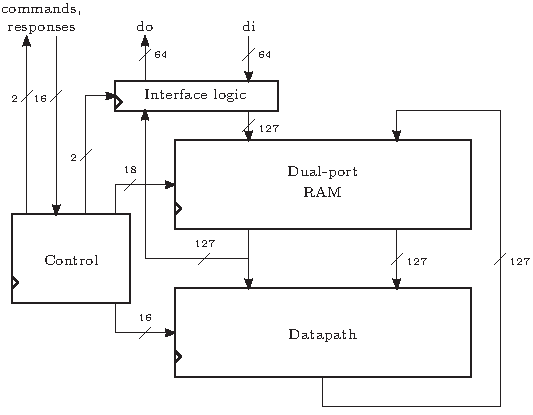
\includegraphics[scale=1.0]{fourq_hardware_architecture_diagram}
	
	\captionof{figure}{Architectural diagram of the core {\fourqs} hardware design proposed in \cite{jarvinen2016four}.}
	\label{fig: fourQ hardware architectural diagram}
\end{figure}
%
The interface logic is used to give inputs to the architecture and to retrieve outputs.
Values used in the computation of the scalar multiplication are stored in the Dual-Port RAM.
The Dual-Port RAM is implemented as BlockRAM in the FPGA. 
By default, the host is connected to the architecture through a 64-bit interface.
Using this interface, we can write or read a value at a specific address within this RAM.
As the design only uses 128-bit data values, this address indicates whether the higher or lower part of the 128-bit word is being written or read.
Although the width of the interface is 64-bits by default, this width can easily be changed \cite{jarvinen2016four}.
The datapath within the design is responsible for the field operations.
It provides the basic operations needed to allow the implementation of field addition, subtraction, doubling and multiplication.
It performs these operations in $\mathbb{F}_{p^2}$ (which in case of {\fourq} boils down to complex number arithmetic).
The datapath consists of two paths: a multiplier path and an adder/subtractor path \cite{jarvinen2016four}.
%
\begin{itemize}
	\item The \textbf{multiplier path} is build around a pipelined 64x64 bit multiplier build using DSP blocks.
	The pipelined multiplier consists of seven pipeline stages (as can be seen in \Cref{sec: IP Blocks}), and the multiplication is done using the schoolbook algorithm.
	To compute the result of a multiplication, four $64 \times 64$-bit partial multiplications are done: $a_i \times b_j$ for $i, j \in \{0, 1\}$.
	This gives $a = a_1 2^{64} + a_0$ and $b = b_1 2^{64} + b_0$.
	The results of these partial multiplications are accumulated in a 256-bit register.
	The order in which the partial products are stored is as follows: $(i, j) = (0, 0), (0, 1), (1, 0), (1, 1)$.
	After $(0, 0)$ and $(1, 0)$, the register is shifted down by 64 bits.
	
	\item The \textbf{adder/subtractor} is responsible for computing the additions, subtractions and modular reductions of the partial multiplications results.
	The adder/subtractor path is designed in such a way that it can also be used when the multiplier path is performing a multiplication \cite{jarvinen2016four}. 
	This is only possible if the modular reduction computed is available and by introducing an additional set of input registers to the adder/subtractor.
	The adder/subtractor also allows accumulation of its results in the output register. 
	Therefore, most of the additions and subtractions required during scalar multiplication come for free.
\end{itemize}
%

\subsection{Control logic} \label{subsec: Control Logic}
The control unit is responsible for controlling the datapath and the memory, and therefore implements all the levels required by {\fourqs} scalar multiplication.
The control logic consists of a program ROM that consists of instruction lines for the datapath and memory addresses.
In addition, the control logic contains a FSM that controls the read addresses from the program ROM.
Also a decoder is present to decode the instructions in the program ROM to control signals such that they can be used to control the datapath and the memory components.
The program ROM contains 8015 lines of hand-optimized instructions.
These instructions are 25 bits wide:
3 bits are used for the multiplier path, 5 bits for the adder/subtractor path, one bit for write enable and two 8-bit memory addresses for the RAM \cite{jarvinen2016four}.
Each instruction line is executed in one clock cycle.
The program ROM is divided into \emph{seven} different routines.
Given a base point $P = (x, y)$ and following \cite[Algorithm 1]{jarvinen2016four}, the routines are as follows:
%
\begin{itemize}
	\item \emph{Initialization}: Lines 1-14 map the affine point $P$ to the representation $\bm{R_1}$: $X \gets x, Y \gets y, Z \gets 1, T_a \gets x$ and $T_b \gets y$.

	\item \emph{Precomputation}: Lines 15-4199 calculate the lookup table $T$ by making use 
	of the endomorphisms and point additions. $T$ consists of 8 points in total, each represented in $\bm{R_5}$.
	
	\item \emph{Initialization main loop}: Lines 4200-4214 initialize the point accumulator (which is used in the main loop) by loading a point from the lookup table $T$. This is done by making use of the first digit of the recoded multiscalar and by mapping this point to representation $\bm{R_4}$. 
	
	\item \emph{Main loop}: Lines 4215-4568 compute the point doubling $Q \gets [2]Q$ and addition $Q \gets Q + m_i \cdot T[v_i]$. The point doubling is calculated using representation $\bm{R_1 \gets R_4}$ (i.e. the input representation to this operation is $\bm{R_4}$, and the output representation is $\bm{R_1}$), while the point addition is calculated using representation $\bm{R_1 \gets R_1 \times R_2}$.
	
	\item \emph{Affine conversion}: Lines 4569-7437 map the resulting point, represented in $\bm{R_1}$, to affine coordinates by computing $x = X/Z$ and $y = Y/Z$. The majority of these lines are used to perform an inversion in $\mathbb{F}_p$.
	
	\item \emph{Point validation}: Lines 7438-7561 verify whether the base point $P=(x, y)$ is in $\mathcal{E}(\mathbb{F}_{p^2})$. This boils down to verify whether point $P$ satisfies the curve equation $-x^2 + y^2 - 1 -dx^2y^2 = 0$.
	
	\item \emph{Cofactor clearing}: To prevent small subgroup attacks (which can be performed in specific scenarios) \cite{lim1997key}, we can perform cofactor clearing as described in \cite[Appendix A]{costello2015fourq}. Lines 7562-8014 perform the cofactor killing by computing $392P$. This is done by making use of the $\bm{R_2 \gets R_1}$ map (lines 7562-7643), followed by eight point doublings (lines 7644-7799) and two point additions (lines 7800-7643).
\end{itemize}
%
As mentioned previously, the instruction decoder controls how the instructions, read from the program ROM, are decoded to appropriate control signals.
The FSM of the control is responsible for setting the address for the program ROM. 
This is done by making use of a counter and hard-coded pointers to the beginning of each routine within the program ROM.
Depending on the operation, the counter gets either incremented such that the next line of a routine is fetched, or its value is set to the appropriate routine.
Once the end pointer of a routine is reached, either the pointer moves to the start of another routine, or the FSM moves to the wait state.

\subsection{Scalar decompose \& recode unit}
The decompose unit of the scalar unit is responsible for both decomposing the scalar $m$ into the 64-bit multiscalars $a_1, a_2, a_3, a_4$ (as described in \Cref{subsec: Scalar decomposition}), and to recode these scalars into digit-columns $(d_{64}, \ldots , d_0)$ with $0 \le d_i < 16$.
These digit-columns are then used during the scalar multiplication to retrieve the correct precomputed points to be added.
To calculate the multiscalar, the four curve constants $\ell_1, \ell_2, \ell_3, \ell_4$ and the values of the basis $\bm{b} = (\bm{b_1}, \bm{b_2}, \bm{b_3}, \bm{b_4})$ are necessary.
As these values are all constants, they are stored in the program ROM and are used from there on.
In addition, the values $\hat{\alpha}_i$ for $i \in \{1, \ldots, 4 \}$ need to be computed, which is done by computing $\ell_i m / \mu$ with $\mu := 2^{256}$.
As the computation of these value involves a multiplication, a \emph{truncated multiplier} was designed in \cite[Algorithm 3]{jarvinen2016four}.
Given two integers $X$ and $Y$ with $0 \le X < 2^{256}$ and $0 \le Y < 2^{195}$, the result $Z_H = \left \lfloor X \cdot Y / (2^{256})\right \rfloor \pmod{2^{64}}$ is calculated.
The truncated multiplier can also be used to calculate the result $Z_L = XY \pmod{2^{64}}$, which is necessary to compute the final values of $a_i$.
Most of the functionality of the truncated multiplier is due to the $17 \times 264$-bit \emph{row multiplier}.
The row multiplier computes the product $Y_j \cdot X$ for a $j \in [0, 11]$ (as needed in \cite[Algorithm 3 line 5]{jarvinen2016four}.) 
The row multiplier is implemented by making use of DSP blocks (11 in total).
The Xillinx Zynq FPGA family, that was used to test the proposed hardware design of {\fourq}, provides $17\times 24$ unsigned integer multiplication with an addition of a 47-bit unsigned integer. 
To be compliant with these dimensions, the 256-bit input integer $X$ is split into $\lceil 256 / 24 \rceil = 11$ blocks of 24-bit words, and the 195-bit input integer $Y$ is split into $\lceil 195 / 17 \rceil = 12$ blocks of 17-bit words.
$X$ and $Y$ now become represented as $X_{10}, X_9, \ldots, X_0$ and $Y_{11}, X_{10}, \ldots Y_0$ in radix $2^{24}$ and $2^{17}$ respectively.

The recode unit is also implemented as FSM, where each state computes one or more lines of the recoding algorithm presented in \cite{costello2015fourq}.


	% !TeX spellcheck = en_US
% !TeX root = ../Tom_Sandmann-master_thesis
\chapter{Side Channel Attacks} \label{chp: Side Channel Attacks}
\lettrine[lhang = 0.4, findent=-30pt, lines=4]{\textbf{
		\initfamily \fontsize{20mm}{20mm} \selectfont W
		\normalfont}}{e} 
describe the side-channel attack used to evaluate the hardware design of {\fourq} (presented in \cite{jarvinen2016four}) in this chapter. 
We first explain Simple Power Analysis (SPA).
We then introduce the concept of \emph{template attacks}.
This is a powerful type of side-channel attack in which profiles are created for the targeted device that are used later on to obtain the secret key.
After that, we look into a different flavor of template attacks that is called \emph{Online Template Attacks} (OTA). 
This improvement of template attacks reduces the number of required template traces to perform the attack.

% !TeX spellcheck = en_US
% !TeX root = ../Tom_Sandmann-master_thesis
\section{Simple Power Analysis}
In Simple Power Analysis (SPA) attacks, power consumption measurements are collected during a cryptographic operation and are directly interpreted.
The attacker tries to derive the key bits more or less directly from the given trace \cite{mangard2008power}. 
This often requires detailed knowledge of the algorithm's underlying implementation executed by the device under attack. 
In the most extreme case, only one power trace can be recorded and used to perform the attack.
This is what we call a \emph{single-shot SPA attack}.
In \emph{multiple-shot SPA attacks}, the attacker is able to record multiple power traces for the same plaintext, or has the ability to supply different plaintexts.
For these attacks to work, the key used in the cryptographic algorithm must have a significant impact on the power consumption of the device under attack.
The impact of the key on the power consumption could be either directly or indirectly.


% !TeX spellcheck = en_US
% !TeX root = ../Tom_Sandmann-master_thesis
\section{Template Attack} \label{sec: Template Attack}
In \cite{chari2002template}, \emph{template attacks} are presented.
These attacks break cryptosystems for which the security is based on the assumption that an attacker is not able to record more than one or a limited number of power traces.
To perform a template attack on a given device, the attacker must have access to another copy of the \emph{exact same} device over which it has full control.
In the preprocessing state of the template attack, templates are created.
In practice, this takes a lot of power traces.
However, the template attack itself only requires a very small number of power traces from the device under attack. 
The obtained templates are then used to reduce the set of possible keys, which makes an attack feasible.
The steps needed to perform a template attack are as follows \cite{whisperer2018template}:
%
\begin{enumerate}
	\item Using a copy of the exact same device as the device under attack, record a large number of power traces using different inputs (e.g. plaintexts and keys).
	
	\item Generate the templates. A \emph{template} is the model of captured side-channel information for one operation and consists of information about the typical signal to expect. 
	In addition, it also contains a noise-characterization for that case \cite{rechberger2004practical}. 
	Templates should be made for all possible operations carried out by the algorithm under consideration.
	The term ``all possible operations'' refers to (a part of) the cryptographic system being executed using key values that trigger \emph{all} relevant execution paths of the system.
	
	\item Capture the trace of a single operation from the device under attack. 
	A single operation could for example be the key-scheduling part of the algorithm running on the device to be attacked.
	
	\item Using the previously generated templates (representing all key-values for the operation to be considered), we classify the side-channel information of the device under attack and assign it to one or more templates. 
	This reduces the number of possible keys (or could even lead to retrieval of the exact key used).
\end{enumerate}
%
We now describe template attacks in more detail.
Assume we have captured a power trace that consists of $b$ sampled points. 
Each sampled point consists of a signal and noise part. 
This gives us a $b$-dimensional noise-vector per trace.
As we know, electric signals are inherently noisy. 
If we take a voltage measurement, we do not expect to see a constant voltage level.
Even if we assume a constant power source (e.g. 4V), the measurement values will slightly oscillate around this constant value (e.g. $3.99, 4.03, 4.02, 3.95$).
One way of modeling this observed noise in a power trace is as follows \cite{whisperer2018template}:
%
\begin{align*}
\bm{X} = X_\text{actual} + \bm{N}
\end{align*}
% 
where $\bm{X}$ and $\bm{N}$ are random variables, which means these values differ every time we take a measurement.
In the case of our example, in which we had a power source of 4V, $X_\text{actual}$ would have a value of 4, where the value of $\bm{N}$ would differ for each measurement taken.
A simple model to deal with these random variables is to make use of the Gaussian distribution. 
The corresponding probability density function (PDF) of a Gaussian distribution is defined as follows:
%
\begin{align*}
f(x) = \frac{1}{\sigma \sqrt{2\pi}} e^{ -(x - \mu)^2 / 2 \sigma^2 }
\end{align*}
%
where $\mu$ is the mean and $\sigma$ is the standard deviation.
For example, if our voltage source has a mean of 4 and a standard deviation of 0.4, the PDF would look like the one shown in \Cref{fig: normal Gaussian example}.
%
\begin{figure}
	\centering
	\begin{tikzpicture}
	\begin{axis}[every axis plot post/.append style={
		mark=none,domain=2:6,samples=50,smooth},
		% All plots: 50 samples, smooth, no marks
		axis x line*=bottom, % no box around the plot, only x and y axis
		axis y line*=left, % the * suppresses the arrow tips
		enlargelimits=upper] % extend the axes a bit to the right and top
		% argument order: average, standard deviation
		\addplot {gauss(4, 0.4)};
	\end{axis}
	\end{tikzpicture}
	\captionof{figure}{Example of a Gaussian distribution with $\mu = 4$ and $\sigma = 0.4$.}
	\label{fig: normal Gaussian example}
\end{figure}
%
We can now use this PDF to determine how likely a certain measurement is. 
If $f(x)$ is very small for one of our key guesses, this guess is probably wrong.

The univariate Gaussian distribution works well for a single measurement.
In the case of more than one random variable, we can make use of the multivariate Gaussian distribution. 
This allows us to model multiple random variables that might correlate.
This model has, in contrary to the more simple univariate models, proven to be adequate for practical usage in template attacks.
Instead of making use of a single variance $\sigma$, we make use of a whole matrix of covariances.
We generalize the covariance matrix construction to a vector column containing $n$ random variables.
Assume we have the column vector:
%
\begin{align*}
\operatorname{\textbf{X}} =
\begin{bmatrix}
\bm{X_1} \\
\vdots \\
\bm{X_n}
\end{bmatrix}
\end{align*}
%
in which the entries are random variables.
Then the covariance matrix $\Sigma$ is the matrix in which the entry $(i, j)$ is the covariance: $\Sigma_{i, j} = \operatorname{cov}(\bm{X_i}, \bm{X_j})$. If $i = j$, this computation can be simplified by computing the variance instead.
The variance is a special case of the covariance in which the two variables are identical (or in other words, the values of the two random variables are the same).
The operations $\operatorname{cov}$ and $\operatorname{var}$ are defined as follows:
%
\begin{align*}
\operatorname{cov}(\bm{X_i}, \bm{X_j}) &= \operatorname{E} \left[ (\bm{X_i} - \mu_i, \bm{X_j}  - \mu_j) \right] = \operatorname{E} \left[ \bm{X_i X_j} \right] - \mu_i \mu_j \\
\operatorname{var}(\bm{X}) &= \operatorname{E} \left[ ( \bm{X} - \operatorname{E}(\bm{X}))^2  \right] = \operatorname{E} \left[(\bm{X} - \operatorname{E}(\bm{X})) \cdot (\bm{X} - \operatorname{E}(\bm{X})) \right]
\end{align*}
%
The covariance matrix looks as follows:
%
\begin{align*}
\Sigma = 
\begin{bmatrix}
\operatorname{E} \left[ (\bm{X_1} - \mu_1) (\bm{X_1} - \mu_1) \right] & \operatorname{E} \left[ (\bm{X_1} - \mu_1) (\bm{X_2} - \mu_2) \right] & \dotsm & \operatorname{E} \left[ (\bm{X_1} - \mu_1) (\bm{X_n} - \mu_n) \right] \\
& & & \\
%
\operatorname{E} \left[ (\bm{X_2} - \mu_2) (\bm{X_1} - \mu_1) \right] & \operatorname{E} \left[ (\bm{X_2} - \mu_2) (\bm{X_2} - \mu_2) \right] & \dotsm & \operatorname{E} \left[ (\bm{X_2} - \mu_2) (\bm{X_n} - \mu_n) \right] \\
& & & \\
%
\vdots & \vdots & \ddots & \vdots \\
& & & \\
%
\operatorname{E} \left[ (\bm{X_n} - \mu_n) (\bm{X_1} - \mu_1) \right] & \operatorname{E} \left[ (\bm{X_n} - \mu_n) (\bm{X_2} - \mu_2) \right] & \dotsm & \operatorname{E} \left[ (\bm{X_n} - \mu_n) (\bm{X_n} - \mu_n) \right] \\
%
\end{bmatrix}
\end{align*}
%
In these definitions, the operator $\operatorname{E}$ denotes the expected (mean) value of its argument, and $\mu_i = \operatorname{E}(\bm{X_i})$ is the expected value of the $i^\mathrm{th}$ entry in vector $\operatorname{\textbf{X}}$. 
The covariance is a measure of the joint variability of two random variables.
If two variables show similar behavior for increasing/decreasing values, this results in positive/negative covariance.
The stronger this linear dependence, the more this value goes to $\pm 1$.
If the inverse of this covariance matrix, $\Sigma^{-1}$, exists, it is also known as the concentration or precision matrix.
The corresponding PDF of this multivariate distribution is different from the one shown for a univariate Gaussian distribution.
Instead of having a single argument, a vector is used which contains all of the variables: $\operatorname{\textbf{x}} = \left[ X_1, X_2, \ldots, X_k \right]^{\rm T}$. 
For $n$ random variables, the equation is as follows:
%
\begin{equation*}
f(\operatorname{\textbf{x}}) = \frac{1}{\sqrt{(2\pi)^n \abs{\Sigma}}} \exp( -\frac{1}{2} (\operatorname{\textbf{x}} - \bm{\mu})^{\rm T} \Sigma^{-1} (\operatorname{\textbf{x}} - \bm{\mu}) )
\end{equation*}
%
where $\bm{\mu}$ is the vector of expected (mean) values, $\Sigma$ is the covariance matrix that corresponds to the random variables, $\exp$ is the matrix exponential function and $\abs{\Sigma}$ is the determinant of the covariance matrix. 
The result of this function is a $n$-dimensional column vector.

\vspace{5mm} \noindent
To be able to classify a trace captured from the device under attack, we need to build a template for each trace, for each of the possible operations.
This template consists of statistical information of the corresponding trace.
This includes the properties of the probability distribution of all the sample points in the trace.
As expected, the quality of the model improves as the number of captured traces increases.
%If we explain the concept of a template in natural language, it would be as follows: ``if you are going to use key $k$, your power trace will look like the distribution $f_k(\operatorname{\textbf{x}})$'' \cite{whisperer2018template}.
This information can be used to find subtle differences between power traces, which makes us able to obtain good key guesses for a single power trace.

\subsection{Making the attack more practical} \label{subsec: Making the attack more practical}

The theoretical approach to template attacks described in the previous subsection is not feasible, as there are couple of problems that need to be dealt with \cite{rechberger2004practical, whisperer2018template}:
%
\begin{itemize}
	\item \textbf{Number of traces}. It is not feasible to create templates for all possible key values. 
	As originally proposed, a template attack requires us to model every single key. 
	Fortunately, different alternatives exist to this approach. 
	One of these approaches is to attack the sensitive parts of the algorithm.
	This could for example be the output of the \textsc{SubBytes} (the substitution box or s-box) operation of the AES encryption algorithm. 
	By focusing on the output of the \textsc{SubBytes} operation, we only need to build templates for each of the 256 outputs of the s-box. 
	This is due to the s-box operating on 8-bits inputs, which gives us 256 input values for the s-box.
	By creating templates for each of these values, we can perform the template attack on the device under attack in $128/8 = 16$ stages (assuming AES128).
	In each stage, we attack a single byte (i.e. a subkey) of the key used.
	Afterwards, we combine the results of all subkey attacks to retrieve the key used.
	
	However, we could do even better. In \cite{brier2004correlation}, it was shown that the power consumption of a microprocessor can correspond to the Hamming weight (the number of \texttt{1}'s in a bitstring) being examined.
	If this assumption holds for the device to be attacked , we only have to make templates for all possible Hamming weights of the s-box output byte, which are 9 values in total.
	This will result in a much faster template generation, as the number of models needed is significantly lower.
	However using the latter method makes us unable to recover the key from a single attack trace: we need more information to retrieve the key used \cite{whisperer2018template}.
	
	Even if we attack the key in stages, each stage will result in a couple of subkeys that are likely to be correct. 
	Combining all of these subkeys to find the secret key is still not efficient.
	To deal with this, one can make use of an extend-and-prune strategy \cite{chari2002template}.
	If we attack the cryptographic algorithm in stages, we first start off with a small candidate set of prefixes for the key.
	After each stage, we end up with another small candidate set of larger-sized prefixes of the key \cite{rohatgi2009improved}.
	By repeating this process, we eventually end up with a limited number of complete keys that we can exhaustively test.
	After each stage, we perform a pruning step to reduce the number of possible keys.
	The pruning step is performed by a classification algorithm, that determines which subkeys at the current iteration survive.
	If the performance of the classification process is efficient, the pruning step will also be more efficient.
	There is however a trade-off to be made between the accuracy of the classification process and the number of possible subkeys that survive after each iteration: if the total number of subkeys surviving in each iteration is too high, it will result in an uncontrollable combinatorial explosion of possible key values towards the end of the attack.
	To be able to perform the attack successfully, it is sufficient to have the feasibility of exhaustive key search on the remaining possible keys. 

	\item \textbf{Points of Interest}. If the number of sampled points in a trace is high, the storage requirements of the traces also increase. 
	In addition, this also has impact on the performance of calculations that need to be done in order to compute the templates (i.e. the matrix inversion of the covariance matrix).
	By making use of points of interest (POIs), we do not need all samples in the power trace to successfully launch a template attack.
	In addition, there is no reason to use multiple POIs captured within a single clock cycle: these points do not provide additional information as it is very likely that they belong tot the same leakage instance.
	We can get the same amount of information from only a single sample captured at the right time \cite{whisperer2018template, rechberger2004practical}.
	
	In general, there are also several ways of picking the most important points in each trace.
	The general goal is to find those points that differ strongly between different operations.
	One of the most simple methods is the \emph{sum of differences} method.
	This method works as follows \cite{whisperer2018template, rechberger2004practical}: 
	%
	\begin{itemize}
		\item For every operation $n \in N$, we have a number of $T_p$ traces $t_1, \ldots, t_p$.
		For each operation $n$, we calculate the average power $M$:
		%
		\begin{equation*}
		M = \frac{1}{T_p} \sum_{j = 1}^{T_p} t_j
		\end{equation*}
		%
		
		\item After we find the mean signal for all of the operations, we calculate the absolute pairwise difference and add these. 
		If we have an operation $n_i \in N$, we calculate its pairwise difference with every \emph{other} operation ($n_1, n_2, \ldots, n_{i - 1}, n_{i + 1}, \ldots, n_{\abs{N} - 1}, n_{\abs{N}}$):
		%
		\begin{equation*}
		D_i = \sum_{n_1, n_2} \abs{M_{n_1, i} - M_{n_2, i}}
		\end{equation*}
		%
		After adding these values together, we again end up with a trace called the \emph{sum of differences} trace. 
		Points in this newly calculated trace that differ strongly between different operations will now have a high value within this trace.

		The next step is to extract the points from this `\emph{sum of differences}' trace that are interesting. 
		In \cite{rechberger2004practical}, only points from this trace are selected that have a minimal height that is higher than the noise floor of the \emph{sum of differences} trace.
		The noise floor of a signal is the measure of the signal created from all sums of all noise sources and unwanted signals within the measurement systems.
		Noise is in this case defined as any signal other than the one being monitored.	
		In \cite{rechberger2004practical}, an algorithm was used that retrieved the $n$ highest peaks.
		This algorithm followed the `noise floor' constraint and also an additional constraint that ensured that the points taken are at least one clock cycle (or more) apart.
		An example algorithm would be the following \cite{whisperer2018template}:
		%
		\begin{enumerate}
			\item Assume we have calculated $D_i$, we now pick the highest point from this $D_i$ and take the value $i = \operatorname{argmax}(D_i)$ as our point of interest (i.e. the sample that currently has the highest peak);
			\item Discard the nearest $N$ points, where $N$ is the minimum spacing between the points of interests (POIs);
			\item Repeat until the required number of POIs have been selected.
		\end{enumerate}
		%

	\end{itemize}
	%
\end{itemize}
%

\subsection{Preprocessing the traces} \label{subsec: template attacks preprocessing the traces}
In side-channel analysis, raw input data is often preprocessed. 
This could either be for simplicity or for efficiency reasons.
However, in some cases, preprocessing has an enormous impact on the actual results of the side-channel attack.
It turns out that by transforming the input traces from the time domain into the frequency domain is a very lucrative transformation. In \cite{rechberger2004practical}, this preprocessing step was done on a template attack on RC4, by making use of FFT.
After preprocessing the traces, the resulting traces could still be used to perform the template attack exactly the same as if they were not preprocessed.
It turned out that the total number of points of interest (as described in \Cref{subsec: Making the attack more practical}) differs when the traces are preprocessed. 
At the price of performing an FFT on every input trace, it was shown that much less points were sufficient in comparison with a template attack in which the traces were not preprocessed \cite{rechberger2004practical}.
The selection of points in the frequency domain is different from the point selection in the time domain.
The lower bound used for the selection of peaks in the time domain was not directly applicable in the frequency domain.
It turned out that the lower bound was much smaller in the frequency domain compared to the one used in the time domain \cite{rechberger2004practical}.

\subsection{Creating the templates}
After determining the POIs in the power traces, it is time to create the templates.
Assume we have $I$ points of interest at samples $s_i$ for $i \in \{0, 1, \ldots, I - 1 \}$.
The next step is to calculate the mean vector and the covariance matrix for every operation (as described previously).
Assume we have $N$ operations, we do the following for each operation $n \in N$ \cite{whisperer2018template, rechberger2004practical}:
%
\begin{itemize}
	\item First, capture a power trace that corresponds to operation $n$.
	If there are $T_p$ of these power traces, we find the average power consumption at every point of interest, which is denoted as $\mu_i$. This value is calculated as follows \cite{rechberger2004practical}:
	%
	\begin{equation*}
	\mu_i = \frac{1}{T_p} \sum_{j = 1}^{T_p} t_{j, s_i}
	\end{equation*}
	%
	where $t_{j, s_i}$ is the value of the point-of-interest $i$ in trace $j$.
	
	\item Next, we find the variance of the power at each point of interest, which we denote as $v_i$. This value is calculated as follows \cite{whisperer2018template}:
	%
	\begin{equation*}
	v_i = \frac{1}{T_p} \sum_{j = 1}^{T_n} ( t_{j, s_i} - \mu_i)^2
	\end{equation*}
	% 
	Note that these values will represent the diagonals of the covariance matrix we build later on.
	
	\item Finally, we calculate the covariance between every point-of-interest pair. This is done as follows \cite{rechberger2004practical}:
	%
	\begin{equation*}
	c_{i, i'} = \frac{1}{T_n} \sum_{j = 1}^{T_n} ( t_{j, s_i} - \mu_i) ( t_{j, s_{i'}} - \mu_{i'})
	\end{equation*}
	%
	with $i, i' \in I$ and $i \neq i'$.
	\item Now its time to put all of the values together to create the corresponding mean vector and covariance matrix \cite{whisperer2018template}:
	%
	\begin{equation*}
	\mu =
	\begin{bmatrix}
	\mu_1 \\
	\mu_2 \\
	\vdots \\
	\mu_I
	\end{bmatrix}
	%
	, \hspace{1cm}
	%
	\Sigma = 
	\begin{bmatrix}
	v_1 & c_{1, 2} & c_{1, 3} & \dotsm & c_{1, I} \\
	c_{2, 1} & v_2 & c_{2, 3} & \dotsm & c_{2, I} \\
	c_{3, 1} & c_{3, 2}  & v_3 & \dotsm & c_{3, I} \\
	\vdots & \vdots & \vdots & \ddots & \vdots \\
	v_{I, 1} & v_{I, 2} & v_{I, 3} & \dotsm & v_I
	\end{bmatrix}
	\end{equation*}
	%
\end{itemize}
%
We end up with $N$ mean column vectors and covariance matrices.
They model each of the $N$ different operations available for the target device.

\subsection{Applying the templates}
Once we have our templates ready, it is time to put them to use.
In order to perform the template attack, we need a number of traces from the target device.
We use these traces to determine how likely our key guesses are.
With `key guesses', we refer to the templates we have generated previously for \emph{all} possible (relevant) key values.
We assume to have $A$ traces from the target device, where each trace consists of samples $a_{j, s_i}$ for $j \in \{1, \ldots , A \}$ \cite{whisperer2018template}.
We now describe how we apply the template to a single trace.
First we have to put the values at the POIs of our trace into a vector:
%
\begin{equation*}
\operatorname{\textbf{a\textsubscript{j}}} =
%
\begin{bmatrix}
a_{j, 1} \\
a_{j, 2} \\
\vdots \\
a_{j, I}
\end{bmatrix}
%
\end{equation*}
%
Now we calculate the PDF for every key guess (i.e. applying each template to every attack trace): $p_{k, j} = f_k(\operatorname{\textbf{a\textsubscript{j}}})$. 
The value $p_{k, j}$ tells us how likely the key $k$ is if we look at trace $j \in A$ \cite{whisperer2018template}. 
As we have multiple traces, each template is applied to each of these attack traces.
Therefore, we end up with a list of $p_{k, j}$ values for every single template. 
Each value in the list is the evaluation of that specific template for that specific attack trace.
After we have applied the templates, it is time to combine the results (i.e use our $p_{k, j}$ values) to determine which template matches the power traces the best (i.e. which key is the best fit).
This is done as follows:
%
\begin{equation*}
P_k = \prod_{j = 1}^{A} p_{k, j}
\end{equation*}
%
For each template, we multiply the corresponding $p_{k, j}$ values, which gives us the likeness that this specific template fits the attack traces \cite{whisperer2018template}. 
Note that when we have a single trace that does not match the template, the $P_k$ value for this template drops very quickly.
This makes it easier to discard non-matching templates (i.e. wrong key guesses).
%
%There is however a problem with this approach.
%If the number of attack traces becomes very large, the multiplication will suffer from precision issues: the multiplication results can not fit in the floating point variable due to overflowing.
%To overcome this problem, we calculate the logarithm of the result instead. 
%As $\log_b(xy) = \log_b x + \log_b y$ (for $b, x$ and $y$ positive and $b \neq 1$), all multiplications become additions of logarithms which solves the precision problem.
%The resulting formula becomes:
%%
%\begin{equation*}
%\log P_k = \sum_{j = 1}^{A} \log p_{k, j}
%\end{equation*}
%%
%The template with the highest $P_k$ value is the key that is the most likely one to be correct.

% 
%Assume we have three random variables, $\bm{X_1}, \bm{X_2}$ and $\bm{X_3}$, with following corresponding column vector:
%%
%\begin{align*}
%\bm{X} = 
%\begin{bmatrix}
%\bm{X_1} \\
%\bm{X_2} \\
%\bm{X_3}
%\end{bmatrix}
%\end{align*}
%%
%The corresponding covariance matrix would be:
%%
%\begin{align*}
%\Sigma
%= 
%\begin{bmatrix}
%\operatorname{var}(\bm{X_1}) & \operatorname{cov}(\bm{X_1}, \bm{X_2}) & \operatorname{cov}(\bm{X_1}, \bm{X_3}) \\
%\operatorname{cov}(\bm{X_2}, \bm{X_1}) & \operatorname{var}(\bm{X_2}) & \operatorname{cov}(\bm{X_2}, \bm{X_3}) \\
%\operatorname{cov}(\bm{X_3}, \bm{X_1}) & \operatorname{cov}(\bm{X_3}, \bm{X_2}) & \operatorname{var}(\bm{X_3})
%\end{bmatrix}
%\end{align*}
%%
%with the following mean for each random variable:
%%
%\begin{equation*}
%\bm{\mu} = 
%\begin{bmatrix}
%\mu_{X_1} \\
%\mu_{X_2} \\
%\mu_{X_3}
%\end{bmatrix}
%\end{equation*}
%%
% !TeX spellcheck = en_US
% !TeX root = ../Tom_Sandmann-master_thesis
\section{Online Template Attack}  \label{sec: Online Template Attack}
In \cite{batina2014online}, a variation of template attacks called \emph{Online Template Attacks} (OTAs) is introduced.
Template attacks are a form of SCAs with a \emph{modus operandi} called \emph{Vertical}.
In these attacks, the implementation under attack is executed several times, such that power traces can be acquired for each of these executions.
Whether these executions use the same input or not depends on whether a simple or advanced SCA is performed.
Besides Vertical SCAs, we also have SCAs with a \emph{modus operandi} called \emph{Horizontal}.
In these attacks, only a single execution is necessary and different (Horizontal) data or computations are considered when attacking the implementation.
The differences between these \emph{modus operandi} of SCAs can be seen in \Cref{fig: vertical_and_horizontal_sca}.
%
\begin{figure}
	\centering
	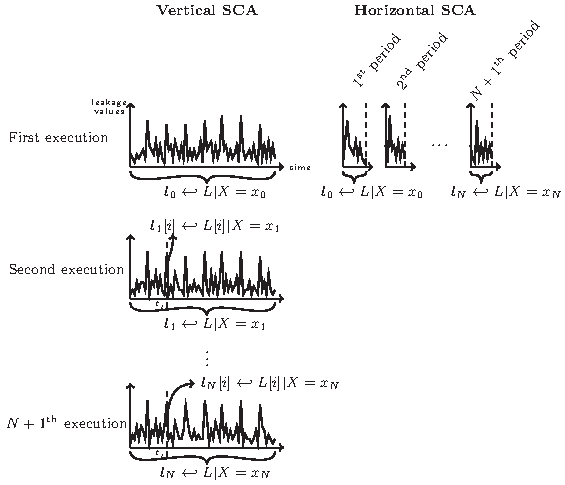
\includegraphics[scale=1.2]{vertical_and_horizontal_sca}
	\captionof{figure}{Visualization of Vertical and Horizontal SCAs (taken from \cite{bauer2013horizontal}).
	A realization of random variable $X$ is referred to as the corresponding lower-case letter $x$.
	A power trace $l_i$ for a given input $x_i$ is denoted as $l_i \hookleftarrow L \mid X = x_i $ (this notation sums up the event of a sample of observations of $L$ under the input $x_i$).
	}
	\label{fig: vertical_and_horizontal_sca}
\end{figure}
%
An OTA combines these two different approaches to SCAs. 
The attack works by acquiring one target trace from the device under attack.
Patterns of certain operations from this target trace are then compared to templates obtained from the attacker's device (which is a similar device running the same implementation).
Thus, an attacker requires only one \emph{target trace} from the \emph{target device}.
Only a single template trace per key-bit is necessary, which is obtained from the device of the attacker.
OTAs can be used to attack the secret scalar used in a scalar multiplication algorithm.
In practice, OTAs make the following assumptions about the attacker \cite{batina2014online, dugardin2016dismantling}:
%
\begin{itemize}
	\item The attacker knows the input point $\mathcal{P}$ that belongs to the trace of the target device;
	\item The attacker knows the implementation of the scalar multiplication algorithm and can compute intermediate values of this algorithm;
	\item The attacker can choose the input point on a device similar to the target device.
\end{itemize}
%
For the attack to work, at least one assignment in the exponentiation algorithm must be dependent on the value of particular scalar bit(s). 
However, there should not be any branches with key-dependent computations.
We now give a global overview of how an OTA works:
%
\begin{itemize}
	\item First, the attacker obtains a target trace with input point $\mathcal{P}$ from the target device;
	\item The attacker now obtains the template traces with input points $[m]P$ for $m \in \mathbb{Z}$.
	 This is done for multiples of the point $\mathcal{P}$, for example $2\mathcal{P}$ or $3\mathcal{P}$;
	 \item The attacker now compares the correlations between the target trace and each pair of template traces.
	 The one with the highest correlation is the one most likely to be correct.
\end{itemize}
%

\subsection{Creating the templates}
In \cite{batina2014online}, several examples are shown on how an OTA works for different scalar multiplication algorithms.
Consider the left-to-right double-and-add always algorithm shown in \Cref{Left-to-right double-and-add-always}.
%
\begin{algorithm}
	\algorithmicrequire $\bm{\mathcal{P}}$, $k = (1, k_{x-2}, \ldots, k_0)_2$. \\
	\algorithmicensure $\bm{Q} = k \cdot \bm{\mathcal{P}}$.
	%	
	\begin{algorithmic}[1]
		\State $\bm{R}_0 \gets \bm{\mathcal{P}}$ 
		\For{$i = x - 2$ \textbf{to} $0$}
			\State $\bm{R}_0 \gets 2 \bm{R}_0$
			\State $\bm{R}_1 \gets \bm{R}_0 + \bm{\mathcal{P}}$
			\State $\bm{R}_0 \gets \bm{R}_{k_i}$ \Comment{Depending on the bit value of $k_i$, $\bm{R}_0$ either takes the value $\bm{R}_0$ or $\bm{R}_1$}
		\EndFor
		\State \textbf{Return} $\bm{R}_0$
	\end{algorithmic}
	%
	\captionof{algorithm}{Left-to-right double-and-add-always algorithm \cite{batina2014online}.}
	\label{Left-to-right double-and-add-always}
\end{algorithm}
%
The algorithm assumes that the most-significant bit of the scalar $k$ is 1 (i.e. $k_\text{MSB} = 1$).
We now describe how an OTA can be applied in the case of \Cref{Left-to-right double-and-add-always}.
It is assumed that the first bit of the scalar is $1$.
However, if we take a look at the `for loop' in \Cref{Left-to-right double-and-add-always}, we see that this bit is not used.
Therefore, we assume that the first iteration of this algorithm (which involves a point doubling and addition) is done with the neutral element of the curve.
Thus, execution of the first iteration will yield the point $\mathcal{P}$.
If we now consider the second iteration (the operations that correspond to $k_\text{MSB} - 1$), we can verify that the expected outputs of this iteration are either $2 \mathcal{P}$ or $3 \mathcal{P}$ (depending on the value of $k_{\text{MSB} - 1}$). 
We now know that in the next iteration (i.e. the operations belonging to key-bit $k_{\text{MSB} - 2}$), a doubling of either $2 \mathcal{P}$ or $3 \mathcal{P}$ will be performed.
On our copy of the same device, we can now execute the algorithm with input point $2 \mathcal{P}$ or $3 \mathcal{P}$. This gives us a trace of the corresponding doubling operations.
Thus we can match the trace of the doubling operation in the ${(i + 1)}^\mathrm{th}$ iteration of the target trace with the appropriate template trace to attack the key bit used in the $i^\mathrm{th}$ iteration:
%
\begin{itemize}
	\item  If $k_{\text{MSB} - 1} = 0$, then the output of the second iteration is $2 \mathcal{P}$. The template trace for $2\mathcal{P}$ (obtained from the iteration involving $k_{\text{MSB} - 2}$) will now give a higher correlation with the target trace than the template trace for $3\mathcal{P}$.
	
	\item If $k_{\text{MSB} - 1} = 1$, then the output of the second iteration is $3 \mathcal{P}$. The template trace for $3\mathcal{P}$ (obtained from the iteration involving $k_{\text{MSB} - 2}$) will now give a higher correlation with the target trace than the template trace for $2\mathcal{P}$.
\end{itemize}
%
In this way, we can iteratively attack and retrieve all of the key bits used.
Note that when we calculate the correlation of the template trace with the target trace, we compare them only at the \emph{suitable} parts of the traces. 
These are the places at which the key-bit related assignments take place.
To determine the most likely key-bit, we compute the correlations with the target trace and the template traces, which in the second iteration would be $2\mathcal{P}$ and $3\mathcal{P}$. 
We consider the template trace that gives the highest correlation value as the one with the right key guess.
We repeat this procedure to find the key-bit for $k_{\text{MSB} - 2}$: we correlate the templates for $4\mathcal{P}$ and $5\mathcal{P}$ with the target trace if we guessed that $k_\text{MSB} - 1 = 0$.
Otherwise, we would correlate using the templates $6\mathcal{P}$ and $7\mathcal{P}$.
Again, the template that gives the highest correlation with the target trace is the most likely one to be correct.
An example of attacking the first two bits of a secret scalar $k$ with respect to \Cref{Left-to-right double-and-add-always} can be seen in \Cref{table: OTA example visualization}.
%
\begin{table}
	\centering
	%
	% Iteration 2 example
	%
	\subfloat[Attacking the second-most significant key bit $K_{\text{MSB} - 1}$. $\operatorname{D}$ and $\operatorname{A}$ stand for the doubling and addition operation respectively as performed in \Cref{Left-to-right double-and-add-always}. Depending on the correlation of the output of the operations performed using the key-bit $K_{\text{MSB} - 1}$ and the corresponding template traces (in this case the template trace $\operatorname{D}(2 \mathcal{P})$), we determine the most likely value for $K_{\text{MSB} - 1}$. In this iteration, we assume that the template for $\operatorname{D}(2 \mathcal{P})$ gives the highest correlation with the target trace.]{
	%
	\begin{tabular}{*7c}
		\toprule
		& \multicolumn{2}{c}{$K_{\text{MSB}} = 1$}  & \multicolumn{2}{c}{$K_{\text{MSB} - 1} \in \{\textcolor{red}{0}, \textcolor{blue}{1}\}$}  & \multicolumn{2}{c}{$K_{\text{MSB} - 2}$} \\
		\midrule
		\textbf{Target Trace} & $\operatorname{D}(\mathcal{O})$ & $\operatorname{A}(\mathcal{O}, \mathcal{P})$ & $\operatorname{D}(\mathcal{P})$ & $\operatorname{A}(2\mathcal{P}, \mathcal{P})$ & $\textcolor{red}{\operatorname{D}(2\mathcal{P})}$ \emph{or} $\textcolor{blue}{\operatorname{D}(3\mathcal{P})} $ & \\
		%
		\multicolumn{7}{c}{} \\
		%
		\textbf{Template Trace of $2 \mathcal{P}$}  & $\operatorname{D}(\mathcal{O})$ & $\operatorname{A}(\mathcal{O}, 2\mathcal{P})$ & \cellcolor{red!20} $\operatorname{D}(2\mathcal{P})$ & $\operatorname{A}(4\mathcal{P}, 2\mathcal{P})$ &  &  \\
		\bottomrule
	\end{tabular}
	%
	\label{table: OTA template matching iteration 2}
	}
	\vfill
	%
	% Iteration 3 example
	%
	\subfloat[Attacking the third-most significant key bit $K_{\text{MSB} - 2}$. 
	Depending on the correlation of the output of the operations performed using the key-bit $K_{\text{MSB} - 2}$ and the corresponding template traces (in this case the template trace $\operatorname{D}(4 \mathcal{P})$), we determine the most likely value for $K_{\text{MSB} - 2}$.]{
		% TODO manually scaled the textwidth, otherwise tablew would still be to wide
		\begin{adjustbox}{max width=.98\textwidth}
			%
			\begin{tabular}{*9c}
				\toprule
				& \multicolumn{2}{c}{$K_{\text{MSB}} = 1$}  & \multicolumn{2}{c}{$K_{\text{MSB} - 1} = 0$}  & \multicolumn{2}{c}{$K_{\text{MSB} - 2} \in \{\textcolor{red}{0}, \textcolor{blue}{1}\}$} & \multicolumn{2}{c}{$K_{\text{MSB} - 3}$} \\
				\midrule
				\textbf{Target Trace} & $\operatorname{D}(\mathcal{O})$ & $\operatorname{A}(\mathcal{O}, \mathcal{P})$ & $\operatorname{D}(\mathcal{P})$ & $\operatorname{A}(2\mathcal{P}, \mathcal{P})$ &
				$\operatorname{D}(2\mathcal{P})$ & $\operatorname{A}(4\mathcal{P}, \mathcal{P})$ & $\textcolor{red}{\operatorname{D}(4\mathcal{P})}$ \emph{or} $\textcolor{blue}{\operatorname{D}(5\mathcal{P})} $ & \\
				%
				\multicolumn{9}{c}{} \\
				%
				\textbf{Template Trace of $4 \mathcal{P}$}  & $\operatorname{D}(\mathcal{O})$ & $\operatorname{A}(\mathcal{O}, 4\mathcal{P})$ & \cellcolor{red!20} $\operatorname{D}(4\mathcal{P})$ & $\operatorname{A}(8\mathcal{P}, 4\mathcal{P})$ &  & & & \\
				\bottomrule
			\end{tabular}
		%
		\end{adjustbox}
		\label{table: OTA template matching iteration 3}
	}
	%
	\captionof{figure}{Visualization of the first two iterations of the OTA applied to \Cref{Left-to-right double-and-add-always} (tables based on examples shown in \cite{dugardin2016dismantling}).}
	\label{table: OTA example visualization}
\end{table}
%

\subsection{Matching the templates}
As mentioned previously, template matching is only performed with parts of the power trace at which the key-bit related assignments take place.
To calculate the correlation between a template and target trace such that we can distinguish the right hypothesis on the current bit under attack, we can make use of the Pearson correlation coefficient. 
The Pearson correlation coefficient is defined as follows:
%
\begin{equation*}
\rho(X, Y) = \frac{\operatorname{cov}(X, Y)}{\sigma_X \sigma_Y}
\end{equation*}
%
where $\operatorname{cov}$ is the covariance, $\sigma_X$ is the standard deviation of $X$ and $\sigma_Y$ is the standard deviation of $Y$.
$X$ and $Y$ would in this case be the template and target trace (in any order).
	% !TeX spellcheck = en_US
% !TeX root = ../Tom_Sandmann-master_thesis
\chapter{\texorpdfstring{Attacking \fourq}{Attacking FourQ}} \label{chp: Attacking FourQ}
\lettrine[lhang = 0.4, findent=-30pt, lines=4]{\textbf{
		\initfamily \fontsize{20mm}{20mm} \selectfont I
		\normalfont}}{n} 
this chapter, we describe how we attack {\fourq}.
In \Cref{chp: Side Channel Attacks}, we have seen how we can apply an \emph{Online Template Attack} (OTA) to a very simple left-to-right double-and-add always algorithm that performed its calculations in constant time.
When applying an OTA to {\fourq}, we have to slightly change our approach to attack the key bits compared to the example we gave in \Cref{chp: Side Channel Attacks}.
In addition, the attack itself is also more difficult, as it (at first sight) requires us to inverse both the scalar recoding and scalar decomposition routines when generating the templates used in attacking the scalar.
We discuss these practicalities in this chapter.

% !TeX spellcheck = en_US
% !TeX root = ../Tom_Sandmann-master_thesis
\section{\texorpdfstring{Applying online template attacks to \fourq}{Applying online template attacks to FourQ}}
In \Cref{algo: FourQ's scalar multiplication} in \Cref{chp: FourQ}, we can see the complete scalar multiplication of \fourq.
In order to retrieve the secret scalar, we need to obtain the $s_i$ and $d_i$ values that are applied in each iteration.
Recall that in the case of an OTA, the attacker can only capture one \emph{target trace} of the device under attack (i.e. the \emph{target device}).
In addition, we assume that the attacker knows the input point that belongs to this trace.
On the attacker's device, the attacker has full control over the implementation (which is the same implementation responsible for the captured \emph{target trace}).
This means that the attacker can change the scalar, but also the base point in the scalar multiplication.
We now describe how we apply an OTA to {\fourq}.
%
\begin{itemize}
	\item \textbf{Attacking the first digit-column}. 
	If we take a look at the actual scalar multiplication algorithm in \Cref{algo: FourQ's scalar multiplication}, we can see that $s_{64}$ determines the sign of the first element taken from the lookup table $T$.
	Which element is taken from this table is determined by the value $d_{64}$, which is unknown to us in the captured \emph{target trace}.
	After the initial assignment in \Cref{lst:fourq scalar mult:initial assignment}, the doubling operation of this initial value (i.e. loop at iteration $i = 63$) is done at \Cref{lst:fourq scalar mult:double oper}.
	This is the first doubling operation we are going to attack.
	If we take a look at the general scalar recoding algorithm employed by {\fourq} in \Cref{algo: Protected Recoding Algorithm for the GLV-SAC Representation} (in \Cref{chp: FourQ})%
	\footnote{In the case of \fourq, we have $l = 65$ and $m = 4$.}
	%
	, we can see that $b_{64}$ is always assigned a value of one, and that this value is used in the main loop as $s_{64}$.
	As we already know that the value of $s_{64} = 1$, we are left to guess the value of $d_{64}$, which is a 3-bit value.
	Our goal in the first `iteration' of our OTA is to try all of the possible $d_{64}$ values (i.e. our templates), such that we can obtain the corresponding power traces of the doubling operations.
	We then use these templates to find the one that matches best with the corresponding part of the \emph{target trace} (i.e. the first doubling operation).
	
	\item \textbf{Attacking the remaining digit-columns}. Once we have found the template (and its corresponding $d_{64}$ value) that matched the best with our \emph{target trace} at the first doubling operation, its time to attack the remaining digit-columns.
	At \Cref{lst:fourq scalar mult:add oper}, we see that both $s_i$ and $d_i$ determine the new value of the variable $Q$. 
	In the next iteration $i - 1$, this variable $Q$ is doubled again. To find out which values of $s_i$ and $d_i$ were used, we have to generate all of the possible templates for these values. This are at most 16 possible templates (3 bits for $d_i$ and 1 bit for $s_i$).
	Note that we need to compare each of the corresponding template traces at the $(i - 1)^\mathrm{th}$ doubling operation to attack the $d_i$ and $s_i$ values used in the addition operation in the $i^\mathrm{th}$ iteration.
	We are then iteratively constructing the matrix that corresponds to the recoded scalars of {\fourq}.
	Using these scalar values, we need to invert the scalar decomposition applied to the secret scalar to obtain the `original scalar' of the scalar multiplication that corresponds to the \emph{target trace}.  
	
	\item \textbf{Attacking the last digit-column}. We cannot use a doubling operation to attack the last digit-column and sign ($s_{0}$ and $d_0$) in the $0^\mathrm{th}$ iteration, as the main loop ends after this iteration. 
	There are however two other ways to attack the last digit-column and its corresponding sign. 
	One way is to use the generated templates for the addition operation involving $d_0$ and $s_0$, and use this operation instead to match the template traces with the target trace.
	Another way would be to brute force these last values, and see which output of the scalar multiplication gives the correct results.
\end{itemize}
%
As mentioned in \cite{batina2014online}, we can also use the addition operation in the $i^\mathrm{th}$ iteration together with the doubling operation in the $(i - 1)^\mathrm{th}$ iteration to attack digit-column $(s_i, d_i)$.
In this way, we can increase the chance of choosing the correct template.
This is however only possible when attacking the digit-columns not used in the first or last iteration (i.e digit-columns $(s_{63}, d_{63})$ up to $(s_{1}, d_{1})$).
% !TeX spellcheck = en_US
% !TeX root = ../Tom_Sandmann-master_thesis
\section{An attempt to inverse the scalar recoding} \label{sec: An attempt to inverse the scalar recoding}
To obtain templates for the OTA, we need to find recoded scalars with specific values at the digit-columns in the corresponding recoded matrix.
As we can change the value of the scalar used in {\fourqs} scalar multiplication, we need to obtain a scalar that, once decomposed and recoded, has the expected digit-column values in it.
To determine which decomposed multiscalar belongs to our wanted recoded matrix, we have to inverse the scalar recoding for this matrix.
We first take a look at the operations in the scalar recoding algorithm shown in \Cref{algo: Protected Recoding Algorithm for the GLV-SAC Representation}.
We can see that in \Cref{lst:scalar recoding general:scalar update}, the value of the scalar gets updated in each iteration by taking the floor of its current value divided by 2 (i.e. a bit shift of 1 to the right) and subtracting the floor of $b_i^j$ divided by 2.
In \Cref{lst:scalar recoding general:digit column value}, we see that the value $b_i^j$ is assigned a value that is the result of taking bit $i$ of the sign-aligner and multiplying it with the very first bit of scalar $k_j$.
So what are the possible values for these variables?
%
\begin{itemize}
	\item $\bm{b_i^j = b_i^J \cdot k_0^j}$. We know that, once the sign-aligner is converted to signed non-zero form (\Cref{lst:scalar recoding general:signed-nonzero start,lst:scalar recoding general:signed-nonzero oper,lst:scalar recoding general:signed-nonzero end})% <--- no space after the comma
	, all of its values at position $i$ will be either $1$ or $-1$: $b_i^J \in \{1, -1\}$. As the value $k_i^j \in \{0, 1\}$ (as all of the scalars are binary numbers in signed form), we have $b_i^j \in \{0, 1, -1\}$.
	
	\item $\bm{k_j = \lfloor k_j / 2\rfloor - \lfloor b_i^j / 2 \rfloor}$. We know that $b_i^j \in \{0, 1, -1\}$. Therefore, we have $\lfloor b_i^j / 2 \rfloor \in \{0, -1\}$. Note that the $-1$ is due to the fact that $\lfloor -1 / 2 \rfloor = -1$.
\end{itemize}
%
As the floor operation applied to the scalar $k_j$ divided by 2 is in essence a bit shift, we can see that this bitshift is done $65$ times (i.e for $j \in [0, 64]$).
As we are working with $64$-bit integers, one would expect that the value of the scalar becomes zero after 64 bitshifts. However, the subtraction of $\lfloor  b_i^j / 2 \rfloor$ from the shifted scalar can also result in an addition of 1.
Therefore, only after $65$ bitshifts the value of $k_j$ will be zero.
We know that all $k_j$'s will have a value of zero once the recoding algorithm has been applied.
Lets see what happens if we try to obtain the original multiscalar by applying the algorithm in reversed order.
As we know, a bitshift is not a completely irreversible operation.
In the case of a right bitshift, we loose the first bit of the scalar (i.e. the bit indicating the parity of the scalar).
Due to the bitshift and subtraction occurring at \Cref{lst:scalar recoding general:scalar update} of the algorithm, we somehow have to guess what the value in the previous iteration would have been.
So what are these possible values.
This depends on the parity of the scalar used.
Assume we have the result $r = (((d >> 1) << 1) + c)$ with $c \in \{0, 1\}$ and $d \in \mathbb{N}$.
By finding all possible outcomes for $r$ and $c$ with $d$ being either odd or even, we know how many possibilities there are when inverting the operation of \Cref{lst:scalar recoding general:scalar update} in the recoding algorithm. 
The results can be seen in \Cref{tbl: inversion of floor function}.
%
\begin{table}
	\centering
	%	
	\begin{tabular}{*3c}
		\toprule
		& $\bm{d \in \mathbb{N}}$ & $\bm{d \in 2\mathbb{N} \setminus \{0\} }$ \\
		\midrule
		$\bm{c = 0}$ & $0$ & $1$ \\
		$\bm{c = 1}$ & $-1$ & $0$ \\
		\bottomrule
	\end{tabular}
	%
	\captionof{table}{Possible outcomes of the equation $r = (((d >> 1) << 1) + c)$ with $c \in \{0, 1\}$ and $d \in \mathbb{N}$ being either odd or even. This table shows the possible values of $k_j$ if we would try to find its original value after we already applied the operation at \Cref{lst:scalar recoding general:scalar update} of \Cref{algo: Protected Recoding Algorithm for the GLV-SAC Representation}.}
	\label{tbl: inversion of floor function}
\end{table}
%
We can see that $r \in \{0, 1, -1\}$, which gives us an idea of the number of possibilities when trying to undo the operation at \Cref{lst:scalar recoding general:scalar update} of the recoding algorithm once it has been applied.
In each iteration of the algorithm, it seems like we need to guess three possibilities to obtain the correct value for iteration $i - 1$: $k_j << 1$, $(k_j << 1) - 1$ and $(k_j << 1) + 1$. 
This seems to be impossible, as this would require us to try $3^{64}$ values.
However, at every moment in time, we only need to make sure that the digit-column for which we are trying to generate templates has a specific value (and all the previous digit-columns we already attacked).
It therefore seems to be the case that the values of the other digit-columns do not matter.
To see if we can make this work, we take a look at the example shown in \cite[Example 1]{faz2015efficient}.
In this example, they also have a multiscalar consisting of four scalars ($m = 4$) having a length of $l = 5$. 
The decomposition of the `original scalar' is given as $kP = 11P_0 + 6P_1 + 14P_2 + 3P_3$. 
If we arrange the scalars in matrix form and apply the recoding, we get the following:
%
\begin{equation*}
%
\begin{bmatrix}
k_0 \\
k_1 \\
k_2 \\
k_3 
\end{bmatrix}
%
\equiv
%
\begin{bmatrix}
0 & 1 & 0 & 1 & 1 \\
0 & 0 & 1 & 1 & 0 \\
0 & 1 & 1 & 1 & 0 \\
0 & 0 & 0 & 1 & 1 
\end{bmatrix}
%
\equiv
%
\begin{bmatrix}
1 & \bar{1} & 1 & \bar{1} & 1 \\
1 & \bar{1} & 0 & \bar{1} & 0 \\
1 & 0 & 0 & \bar{1} & 0 \\
0 & 0 & 1 & \bar{1} & 1
\end{bmatrix}
%
\end{equation*}
%
We are going to attack the leftmost digit-column (just like the one that would be used in the very first iteration of {\fourqs} scalar multiplication algorithm).
In this case, this is digit-column $d_4$.
Our first step would be to find a multiscalar that produces the output in the matrix that we want to have for $d_4$.
We assume that this is the exact same template as the one produced by the `secret' scalar: $\mathbb{K}_4 = \left[ 011 \right]$ or $d_4 = 3$.
Now we try to find the remaining entries in the recoding matrix. 
For simplicity, we show our attempt by only taking the first scalar into account (i.e. $k_1$). 
Recall the operation that updates the scalar in each iteration:
%
\begin{equation*}
k_j = \lfloor k'_j / 2 \rfloor - \lfloor b_i^j \rfloor \equiv \lfloor k'_j / 2 \rfloor - \lfloor (b_i^J \cdot k_0^{\prime j} ) / 2 \rfloor 
\end{equation*}
%
with $k_j'$ denoting the value of $k_j$ in the current iteration before it was updated (i.e the value of $k_j$ after the previous iteration $i - 1$ finished).
The attempt is shown below.
%
\begin{itemize}
	\item \textbf{Iteration} $\bm{i = 4}$. 	We know that $k_1 = \lfloor k'_1 / 2 \rfloor - \lfloor (b_4^J \cdot k_0^{\prime 1} ) / 2 \rfloor = 0$ with $k'_1 \in \{0, 1\}$ (note that $-1$ is not possible as the intermediate values of the scalar remain positive throughout the entire algorithm). 
	In addition, we also know that $b_4^J = 1$.
	This gives us two possibilities:
	%
	\begin{itemize}
		\item $\bm{ \lfloor k'_1 / 2 \rfloor = 0 }$ \textbf{and} $ \bm{ \lfloor (b_3^J \cdot k_0^{\prime 1}) / 2 \rfloor = 0 }$. 
		$\lfloor k'_1 / 2 \rfloor = 0$ can only happen if $k'_1 \in \{0, 1\}$. $\lfloor (b_3^J \cdot k_0^{\prime 1}) / 2 \rfloor = 0$ can only happen if $b_3^J \cdot k_0^{\prime 1} \in \{0, 1\}$. This implies that $b_4^J = 1$ and $ k_0^{\prime 1} = 1$. The latter is only possible if $k'_1 = 1$.
		
		\item  $\bm{ \lfloor k'_1 / 2 \rfloor = 1 }$ \textbf{and} $ \bm{ \lfloor (b_3^J \cdot k_0^{\prime 1}) / 2 \rfloor = 1 }$. 
		$ \lfloor k'_1 / 2 \rfloor = 1$ is only possible if $k'_1 \in \{0, 1\}$. However, this contradicts with the fact that $k'_1 \in \{0, 1\}$ \Lightning.
	\end{itemize}
	%
	
	\item \textbf{Iteration} $\bm{i = 3}$. We know that $k_1 = \lfloor k'_1 / 2 \rfloor - \lfloor (b_3^J \cdot k_0^{\prime 1}) / 2 \rfloor = 1$ with $k'_1 \in \{1, 2, 3\}$. This gives us two possibilities:
	%
	\begin{itemize}
		\item $\bm{ \lfloor k'_1 / 2 \rfloor = 0 }$ \textbf{and} $ \bm{ \lfloor (b_3^J \cdot k_0^{\prime 1}) / 2 \rfloor = -1 }$. 
		$\lfloor k'_1 / 2 \rfloor = 0 $ can only happen if $k'_1 = 1$. $\lfloor (b_3^J \cdot k_0^{\prime 1}) / 2 \rfloor = -1$ can only happen if $b_3^J \cdot k_0^{\prime 1} \in \{-2, -1 \}$. This means that $k_0^{\prime 1} = 1$ and $b_3^J = -1$.
		
		\item $\bm { \lfloor k'_1 / 2 \rfloor = 1 }$ \textbf{and} $ \bm{ \lfloor (b_3^J \cdot k_0^{\prime 1}) / 2 \rfloor = 0 }$.
		$\lfloor k'_1 / 2 \rfloor = 1$ can only happen if $k'_1 \in \{2, 3\}$. $ \lfloor (b_3^J \cdot k_0^{\prime 1}) / 2 \rfloor = 0$ can only happen if $b_3^J \cdot k_0^{\prime 1} \in \{0, 1\}$. This gives the following combinations of values:
		%
		\begin{itemize}
			\item $b_3^J = -1$ and $ k_0^{\prime 1} = 0$ (implies $k'_1 = 2$)
			\item $b_3^J = 1$ and $ k_0^{\prime 1} = 0$ (implies $k'_1 = 2$)
			\item $b_3^J = 1$ and $ k_0^{\prime 1} = 1$ (implies $k'_1 = 3$)
		\end{itemize}
		%
		For the sake of simplicity, we assume to guess $k'_1 = 1$ which gives $k_0^{\prime 1} = 1$.
	\end{itemize}
	%
	\item \textbf{Iteration} $\bm{i = 2}$. We know that $k_1 = \lfloor k'_1 / 2 \rfloor - \lfloor (b_2^J \cdot k_0^{\prime 1}) / 2 \rfloor = 1$ with $k'_1 \in \{1, 2, 3\}$. This gives us two possibilities:
	%
	\begin{itemize}
		\item $\bm{ \lfloor k'_1 / 2 \rfloor = 0 }$ \textbf{and} $ \bm{ \lfloor (b_2^J \cdot k_0^{\prime 1}) / 2 \rfloor = -1 }$. 
		$\lfloor k'_1 / 2 \rfloor = 0 $ can only happen if $k'_1 = 1$. $\lfloor (b_2^J \cdot k_0^{\prime 1}) / 2 \rfloor = -1$ can only happen if $b_2^J \cdot k_0^{\prime 1} \in \{-2, -1\}$. This means that $k_0^{\prime 1} = 1$ and $b_2^J = -1$.
		
		\item $\bm { \lfloor k'_1 / 2 \rfloor = 1 }$ \textbf{and} $ \bm{ \lfloor (b_2^J \cdot k_0^{\prime 1}) / 2 \rfloor = 0 }$.
		$\lfloor k'_1 / 2 \rfloor = 1$ can only happen if $k'_1 \in \{2, 3\}$. $ \lfloor (b_2^J \cdot k_0^{\prime 1}) / 2 \rfloor = 0$ can only happen if $b_2^J \cdot k_0^{\prime 1} \in \{0, 1\}$. 
		This gives the following combinations of values:
		%
		\begin{itemize}
			\item $b_2^J = -1$ and $ k_0^{\prime 1} = 0$ (implies $k'_1 = 2$)
			\item $b_2^J = 1$ and $ k_0^{\prime 1} = 0$ (implies $k'_1 = 2$)
			\item $b_2^J = 1$ and $ k_0^{\prime 1} = 1$ (implies $k'_1 = 3$)
		\end{itemize}
		%
		For the sake of simplicity, we assume to guess $k'_1 = 2$ which gives $k_0^{\prime 1} = 0$.
	\end{itemize}
	%
	\item \textbf{Iteration} $\bm{i = 1}$. We know that $k_1 = \lfloor k'_1 / 2 \rfloor - \lfloor (b_1^J \cdot k_0^{\prime 1}) / 2 \rfloor = 2$ with $k'_1 \in \{3, 4, 5\}$. This gives us two possibilities:
	%
	\begin{itemize}
		\item $\bm{ \lfloor k'_1 / 2 \rfloor = 1 }$ \textbf{and} $ \bm{ \lfloor (b_1^J \cdot k_0^{\prime 1}) / 2 \rfloor = -1 }$. 
		$\lfloor k'_1 / 2 \rfloor = 1 $ can only happen if $k'_1 \in \{2, 3\}$ (i.e. $k'_1 = 3$). $\lfloor (b_1^J \cdot k_0^{\prime 1}) / 2 \rfloor = -1$ can only happen if $b_1^J \cdot k_0^{\prime 1} \in \{-2, -1\}$. This means that $k_0^{\prime 1} = 1$ and $b_1^J = -1$.
		
		\item $\bm { \lfloor k'_1 / 2 \rfloor = 2 }$ \textbf{and} $ \bm{ \lfloor (b_1^J \cdot k_0^{\prime 1}) / 2 \rfloor = 0 }$.
		$\lfloor k'_1 / 2 \rfloor = 2$ can only happen if $k'_1 \in \{4, 5\}$. $ \lfloor (b_1^J \cdot k_0^{\prime 1}) / 2 \rfloor = 0$ can only happen if $b_1^J \cdot k_0^{\prime 1} \in \{0, 1\}$. 
		This gives the following combinations of values:
		%
		\begin{itemize}
			\item $b_1^J = -1$ and $ k_0^{\prime 1} = 0$ (implies $k'_1 = 4$)
			\item $b_1^J = 1$ and $ k_0^{\prime 1} = 0$ (implies $k'_1 = 4$)
			\item $b_1^J = 1$ and $ k_0^{\prime 1} = 1$ (implies $k'_1 = 5$)
		\end{itemize}
		%
		For the sake of simplicity, we assume to guess $k'_1 = 3$ which gives $k_0^{\prime 1} = 1$.
	\end{itemize}
	%
	\item \textbf{Iteration} $\bm{i = 0}$. We know that $k_1 = \lfloor k'_1 / 2 \rfloor - \lfloor (b_0^J \cdot k_0^{\prime 1}) / 2 \rfloor = 3$ with $k'_1 \in \{5, 6, 7\}$. This gives us two possibilities:
	%
	\begin{itemize}
		\item $\bm{ \lfloor k'_1 / 2 \rfloor = 2 }$ \textbf{and} $ \bm{ \lfloor (b_0^J \cdot k_0^{\prime 1}) / 2 \rfloor = -1 }$. 
		$\lfloor k'_1 / 2 \rfloor = 2 $ can only happen if $k'_1 \in \{4, 5\}$ (i.e. $k'_1 = 5$). $\lfloor (b_0^J \cdot k_0^{\prime 1}) / 2 \rfloor = -1$ can only happen if $b_0^J \cdot k_0^{\prime 1} \in \{-2, -1\}$. This means that $k_0^{\prime 1} = 1$ and $b_1^J = -1$.
		
		\item $\bm { \lfloor k'_1 / 2 \rfloor = 3 }$ \textbf{and} $ \bm{ \lfloor (b_0^J \cdot k_0^{\prime 1}) / 2 \rfloor = 0 }$.
		$\lfloor k'_1 / 2 \rfloor = 3$ can only happen if $k'_1 \in \{6, 7\}$. $\lfloor (b_0^J \cdot k_0^{\prime 1}) / 2 \rfloor = 0$ can only happen if $b_1^J \cdot k_0^{\prime 1} \in \{0, 1\}$. 
		This gives the following combinations of values:
		%
		\begin{itemize}
			\item $b_0^J = -1$ and $ k_0^{\prime 1} = 0$ (implies $k'_1 = 6$)
			\item $b_0^J = 1$ and $ k_0^{\prime 1} = 0$ (implies $k'_1 = 6$)
			\item $b_0^J = 1$ and $ k_0^{\prime 1} = 1$ (implies $k'_1 = 7$)
		\end{itemize}
		%
		For the sake of simplicity, we assume to guess $k'_1 = 6$ which gives $k_0^{\prime 1} = 1$.
	\end{itemize}
	%
\end{itemize}
%
As you can see, we have three possibilities for obtaining a specific value for the last bit in digit-column $\mathbb{K}_4$.
For the other most-significant bits in the remaining digit-columns, we have four combinations to guess. This gives a total number of $3 \cdot 4^4 = 768$ combinations for this very simple example. In the case of {\fourq} where we have $l = 65$, this would give us $3 \cdot 4^{64}$ possible combinations (a 130-bit value), which is clearly unfeasible to brute force. 
%
\begin{table}[H]
	\centering
	\begin{tabular}{*6c}
		\toprule 
		& \multicolumn{5}{c}{iteration $i$} \\
		\cline{2-6}
		& \textbf{0} & \textbf{1} & \textbf{2} & \textbf{3} & \textbf{4} \\
		\midrule
		$b_i^J$ & 1 & -1 & 1 & -1 & 1 \\
		$k_0^j$ & 0 & 1 & 0 & 1 & 1 \\
		$b_i^j$ & 0 & -1 & 0 & -1 & 1 \\
		$k_j$ & 3 & 2 & 1 & 1 & 0  \\
		\bottomrule
	\end{tabular}
	\captionof{table}{intermediate values for the scalar recoding iteration with $j = 1$ and $k_1 = 6$.}
\end{table}
%
\begin{figure}[H]
	\centering
	\subfloat[Outcome ranges for the function $\lfloor \frac{x \cdot y}{2}\rfloor$ with $x \in \{1, -1\}$ and $y \in \{0, 1\}$ but $y$'s exact value being unknown.]{
	%
	\centering
	\begin{tabular}{*2c}
		\toprule
		& $\lfloor \frac{x \cdot y}{2}\rfloor$ \\
		\midrule
		$x = 1$ & $y$ \\
		$x = -1$ & $-y$ \\
		\bottomrule
	\end{tabular}
	%
	}
	%	
	\hspace{1cm}
	%		
	\subfloat[Outcome ranges for the function $\lfloor \frac{x \cdot y}{2}\rfloor$ with $y \in \{0, 1\}$ and $x \in \{-1, 1\}$ but $x$'s exact value being unknown.]{
	%
	\centering
	\begin{tabular}{*2c}
		\toprule
		& $\lfloor \frac{x \cdot y}{2}\rfloor$ \\
		\midrule
		$y = 0$ & $0$ \\
		$y = 1$ & $x$ \\
		\bottomrule
	\end{tabular}
	%
	}
	\captionof{figure}{Possible outcomes for the function $\lfloor \frac{x \cdot y}{2}\rfloor$ with either $x$ or $y$ being unknown.}
\end{figure}
%
Fortunately, we can circumvent the inversion of the recoding by changing the hardware implementation in such a way that it takes a decomposed scalar instead of a scalar that still needs to be decomposed. 
The implementation still remains the same, but instead of assigning the results of the decomposition to the corresponding multiscalar, we take the values of the decomposed scalar directly and assign them to their corresponding signals.
It would however still be interesting to see if it is possible to invert the scalar recoding in such a way that you can create a recoded multiscalar.
If we convert this multiscalar back to the original scalar and apply decomposition and recoding, it should still have the wanted values at the specific digit-columns in the recoded matrix.
This would make a template attack against hardware implementations of {\fourq} possible in an even more restricted setting where the attacker does have a similar device, but where its implementation cannot be changed. 
This could however be a whole research project on its own, and is left as an open problem for others.
% !TeX spellcheck = en_US
% !TeX root = ../Tom_Sandmann-master_thesis
\section{Determining the offsets} \label{sec: Determining the offsets}
Given the power trace of both the target trace and the template trace, we need to extract the relevant doubling and/or addition operations from these traces and correlate them.
This requires us to determine the offsets into these trace that indicate where the required operation starts and how long it lasts.
To determine these offsets, we add a trigger to our hardware design that is high between the start and end of these operations.
Determining these exact values was done adding by adding output statements to the \emph{control FMS} (see \Cref{chp: FourQ On Hardware}).
This component knows exactly when the scalar multiplication is executing within the main loop.
Unfortunately, there is only \emph{one} state which indicates that either the doubling or addition operation is performed, but not exactly when it starts or ends.
From \cite{jarvinen2016four}, we know that an iteration of the main loop of {\fourq} starts when the value of the program counter equals 4215 and ends when this value is 4568.
We also know that the main loop starts with the doubling operation.
Thus, it remains unclear when (1) a doubling operations ends and when (2) an addition operation starts.
To obtain these unknown offsets (and also to verify the known ones), we make use of a reference implementation of {\fourq} available on GitHub%
\footnote{\url{https://bifurcation.github.io/fourq/}} that belongs to an Internet-Draft of {\fourq} \cite{ladd-cfrg-4q-01}.
This implementation is dubbed \texttt{Curve4Q} and follows the approach described in the original paper.
It therefore does \emph{not} make use of the newly introduced representation $\bm{R_5}$ used in the proposed hardware design of {\fourq} \cite{jarvinen2016four}.
Thus, we add the conversion functions as shown in \Cref{appendix: curve4q modifications} to this reference implementation.
We then change the code in such a way that these newly introduced conversion functions are used in the table generation phase and in the initial assignment to $Q$.
In addition, we also add print statement to the start and end of the actual \texttt{DBL} and \texttt{ADD} methods.
By also printing the output of the Field Arithmetic Unit (FAU)%
\footnote{This is done by making use of the \mintinline{text}{image_pb.vhd} VHDL package written by Ben Cohen, which can be found \href{http://web.archive.org/web/20070202003755/http://members.aol.com/vhdlcohen/vhdl/Models.html}{online}.
A more recent version of such a package is the \mintinline{text}{txt_util.vhd} VHDL package, written by Øyvind Harboe.}
%
and the program counter, we can use the output of both the reference implementation and the FAU to determine at which program counter values the \texttt{DBl} and \texttt{ADD} operations start and end.
The results can be seen in \Cref{tbl: FourQ DBL/ADD start/end values}.
%
\begin{table}
	\centering
	%
	\begin{tabular}{*3c}
		\toprule
		& \textbf{start} & \textbf{end} \\
		\midrule
		\texttt{DBL} & 4216/4217 & 4380/4381 \\
		\texttt{ADD} & 4373/4374 & 4564/4565 \\
		\bottomrule
	\end{tabular}
	%
	\captionof{table}{Values of the program counter in the hardware design of {\fourq} at which the \texttt{DBL} and \texttt{ADD} operations start and end. The value of the program counter points to instructions in program ROM that are used to control the operations needed to compute the scalar multiplications of {\fourq.} }
	\label{tbl: FourQ DBL/ADD start/end values}
\end{table}
%
We used these program counter values to add a trigger in the given hardware design that has a high signal on the start and end of each operation.
As the main loop of {\fourq} consists of 64 points additions \emph{and} 64 doubling operations, this gives us 128 rising and falling edges in the corresponding power trace of this trigger.

As described in \cite{batina2014online}, we can also focus on a single operation within this doubling operation. 
Focusing on the first squaring operation in doubling formulas described in \cite{ladd-cfrg-4q-01} gives us different values for the program counter. These values can be seen in \Cref{tbl: FourQ DBL/ADD start/end values first squaring}.
%
\begin{table}
	\centering
	%
	\begin{tabular}{*3c}
		\toprule
		& \textbf{start} & \textbf{end} \\
		\midrule
		\texttt{DBL} & 4216/4217 & 4251 \\
		\texttt{ADD} & 4373/4374 & 4489 \\
		\bottomrule
	\end{tabular}
	%
	\captionof{table}{Values of the program counter in the hardware design of {\fourq} at which the \texttt{DBL} and \texttt{ADD} operations start and end. In this case, instead of taking the whole doubling operation into account, only the first squaring in the doubling and addition operation is used to find the corresponding program counter values.}
	\label{tbl: FourQ DBL/ADD start/end values first squaring}
\end{table}
%
The corresponding power trace when using the start/end values for the \emph{addition} operation as mentioned in \Cref{tbl: FourQ DBL/ADD start/end values}, and for the \emph{doubling} operation as mentioned in \Cref{tbl: FourQ DBL/ADD start/end values first squaring}, can be seen in \Cref{fig: oper_trigger_trace}.
%
\begin{figure}
	\centering
	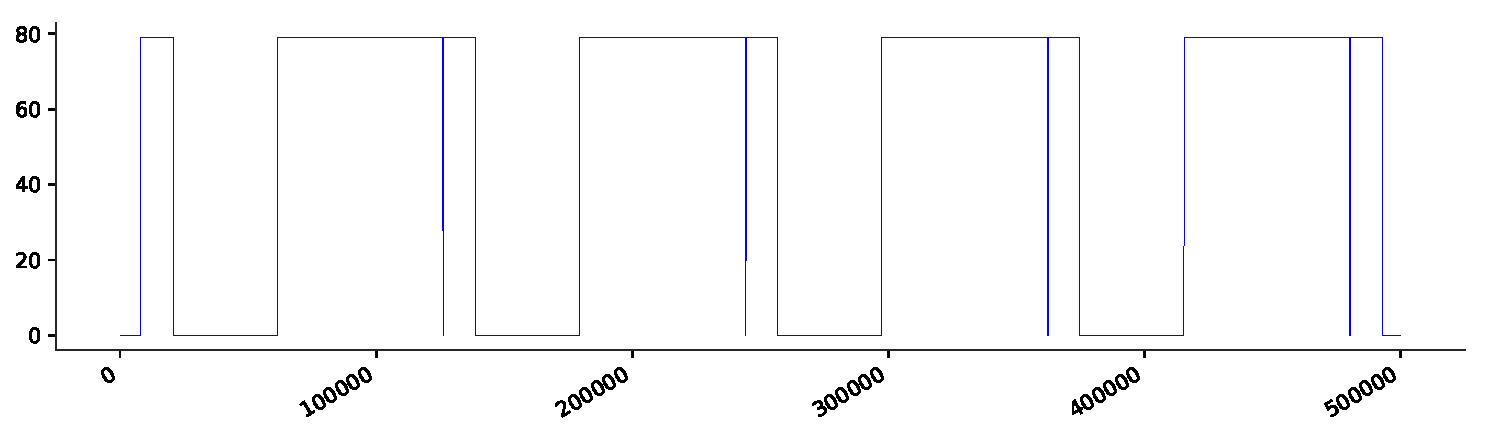
\includegraphics[scale=0.6]{traces/oper_trigger_trace}
	\captionof{figure}{Power trace that indicates at which samples the doubling and addition operations start and end. Instead of taking the whole doubling operation into account, we only determine where the very first squaring happens. This explains why the doubling operation consist of less samples than the addition operation. }
	\label{fig: oper_trigger_trace}
\end{figure}
%
Given this power trace, we need to determine the indices at which a rising edge starts and how long it stays high (i.e. determine the relative index of the start of the corresponding falling edge).
Initially, our approach was to calculate the difference between consecutive elements in this trigger trace without any preprocessing. 
If the difference of two successive elements is high, it indicates that we are approaching a rising/falling edge (depending on the sign of this difference).
The success of this approach however depends on the sampling rate used.
If a low sampling rate is used, the difference between two successive elements can be higher.
In the case of a higher sampling rate, this difference will be much smaller.
Therefore, it is hard to choose a correct threshold to determine the indices of the rising and falling edges in this trigger trace.
To solve this, we decided to preprocess the trace by rounding all values below a threshold to zero.
One has to make sure that this threshold is lower than the values between a rising and falling edge.
Applying the method we described first now correctly yields the offsets at which operations start and end.

The previously described method still depends on the vertical offset of the operation trigger trace. 
A method that works regardless the vertical offset is shown in \Cref{algo: determining offsets}.
In the end, we decided to stick with this generic method.
The algorithm works by first determining the average of the minimum and maximum value in the trigger trace.
We then determine the greatest lower bound (GLB) and least upper bound (LUB) for all values smaller and bigger than this average respectively.
Our threshold $\mu$ now becomes the average of GLB and LUB.
All values in the trigger trace that are bigger or equal to this threshold are clipped to the maximum value, while values smaller are clipped to the minimum value. 
We then calculate the consecutive differences of all the samples in this trigger trace.
We can now determine the rising and falling edge indices by checking whether these absolute differences are bigger than our threshold $\mu$.
The offsets can now easily be found by taking the difference between these indices.
Given a pair of successive edge indices, only those indices are taken into account for which the first edge index corresponds to a rising edge (i.e. has a positive difference or its value is bigger than $\mu$).
%
\begin{algorithm}
	\algorithmicrequire A power trace $T$ of the trigger that indicates when one or more doubling/addition operations start/end. \\
	\algorithmicensure The offsets and durations to these operations.
	%	
	\begin{algorithmic}[1]
		\State $\text{min\_max\_avg} = (\max(T) + \min(T)) / 2$
		\State $T_H = \{s \mid s \in T, s \ge \text{min\_max\_avg} \}$
		\State $T_L = \{s \mid s \in T, s < \text{min\_max\_avg} \}$
		\State $\text{lub} = \sup(T_H)$ \Comment{Least Upper Bound (LUB)}
		\State $\text{glb} = \inf(T_L)$ \Comment{Greatest Lower Bound (GLB)}
		\State $\mu = (\text{glb} + \text{lub}) / 2$
		\State For all $s$ in $T$: if $s \ge \mu$ clip value to $\max(T)$, else clip value to $\min(T)$
		\State $\texttt{succ\_diffs}= \{T[n + 1] - T[n] \mid n \in [1, \#T) \}$ \Comment{Calculate the first order difference}
		\State $\texttt{edges} = \{\operatorname{idx}(d) + 1, d\in D \mid \abs{d} \ge \mu \}$ \Comment{Determine offsets}
		\State $\texttt{offsets} = \{(\texttt{edges}[n], \texttt{edges}[n + 1] - \texttt{edges}[n]) \mid n \in [0, \#\texttt{edges} ], \texttt{offsets}[n] > \mu \}$
		\State \textbf{Return} $\texttt{offsets}$
	\end{algorithmic}
	%
	\captionof{algorithm}{Given a power trace that contains the signals of the operations to attack, determine the offsets to these operations.}
	\label{algo: determining offsets}
\end{algorithm}
%
% !TeX spellcheck = en_US
% !TeX root = ../Tom_Sandmann-master_thesis
\section{Matching the templates} \label{sec: Matching the templates}
Using the method as described in \Cref{algo: determining offsets} of \Cref{sec: Determining the offsets} to determine the offsets, we applied the OTA to the {\fourq} hardware design using the SAKURA-G board.
For the very first iteration, the target trace of the relevant doubling operation together with the corresponding template traces can be seen in \Cref{fig: OTA first iteration target example} and \Cref{fig: OTA first iteration templates example} respectively.
An overlap of the template traces can be seen in \Cref{fig: OTA first iteration template traces overlap}.
All of these traces are captured with a sampling rate of 1GSa/s without any bandwidth or noise filter applied.
The signal coupling of the channels was set to $\mathrm{DC}50\ohm$.
The operation speed of the {\fourq} design was set to 1.5MHz (which is the default speed).
Due to the Nyquist-Shannon sampling theorem, we need to capture a power trace at a sample rate that is at least twice the bandwidth of the input signal. 
In addition, it may be preferable to use a sample rate that is (at least) 10 times the acquisition bandwidth, such that fast signal rise times are oversampled in order to make them consistent with the oscilloscope bandwidth \cite{waverunner6manual}.
This justifies our acquisition rate of 1GSa/s.
%
\begin{figure}
	\centering
	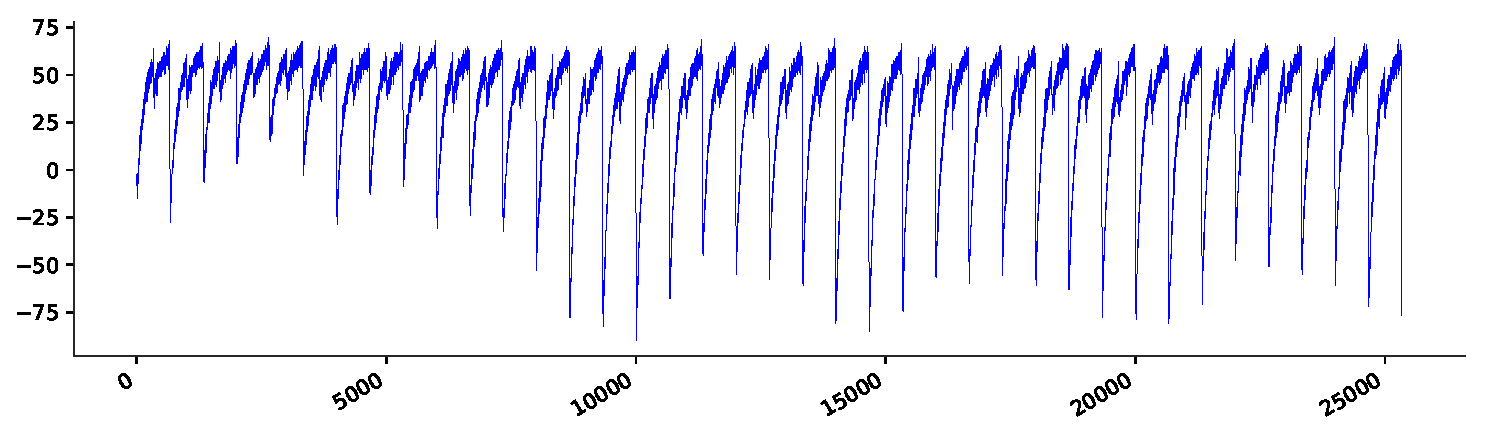
\includegraphics[scale=0.6]{traces/first_doubling/target_trace_dbl_oper_d64}
	\captionof{figure}{Target trace of the first doubling, which is produced using the value $d_{64} = 7$ with the base point and scalar as listed in \Cref{App sec: example template traces} in \Cref{Appendix}.}
	\label{fig: OTA first iteration target example}
\end{figure}
%
\begin{figure}
	\centering
	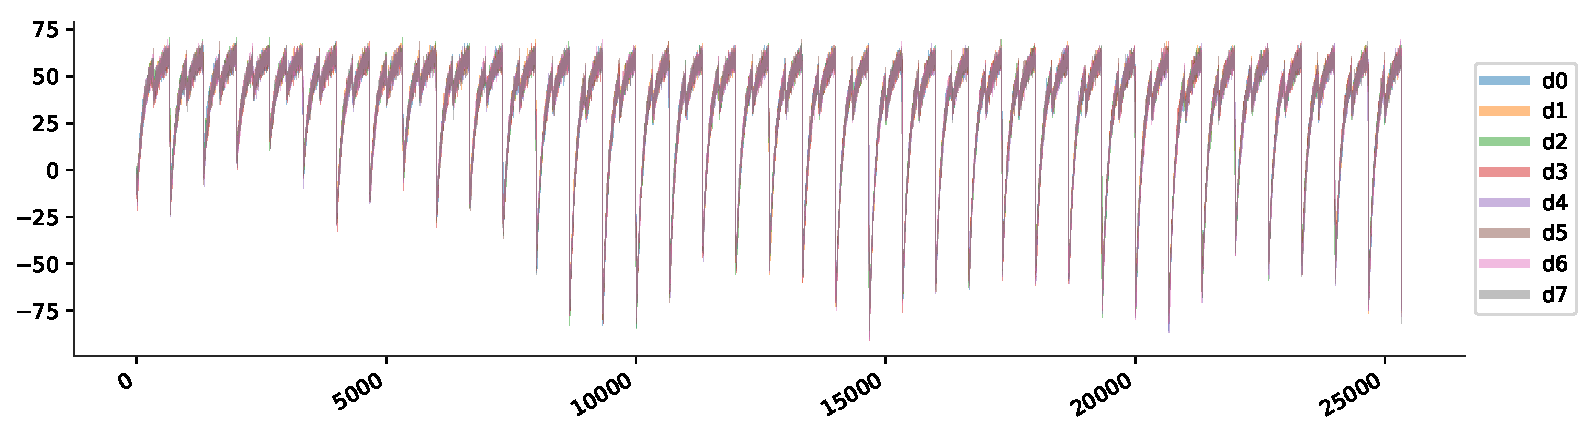
\includegraphics[scale=0.59]{traces/first_doubling/template_traces_overlap_d64}
	\captionof{figure}{An overlap of all the template traces shown in \Cref{App sec: example template traces}.}
	\label{fig: OTA first iteration template traces overlap}
\end{figure}
%
Without even looking at the correlation results, we can immediately see that the template traces are almost identical. 
After viewing the traces in Inspector SCA (a software product developed by Riscure), we can see that there are very small differences between these template traces.
The similarity among the template traces is also reflected in the correlation values obtained after correlating the templates with each other.
These correlation values are at least 99\%.

After correlating the template traces with the target trace using the Pearson correlation coefficient while attacking the first 5 digit-columns (i.e. the first 5 iterations of the OTA), we again observed that all of the correlation values were close to 99\%. 
Instead of only using the doubling operation, we also made use of the fact that we can use the addition operation to have two `operations of reference' instead of one.
Making use of this approach slightly decreased the correlation values.
However, the results were similar to the results observed when \emph{only} making use of the doubling operation.
We decided to research which part of the frequency of the target trace contained the expected leakage.
After applying FFT to the target trace, we found out that the interesting samples were in the higher frequencies of the trace.
This was verified by making use of a low-pass filter with a cut-off frequency of 81MHz.
If the interesting frequencies of a trace are filtered out, the traces will even look more similar, which will result in higher correlation values in the template-matching phase.
This is also exactly what we observed in the correlation values after we applied the aforementioned low-pass filter.
Therefore, we decided not to use this low-pass filter in the remaining experiments we conducted.

\subsection{Bandwidth filter comparison}
As the template-matching results are so close to each other, we decided to attack the first 5 digit-columns (i.e $d_{64}$ up to $d_{60}$) for the same target trace.
Each attack was performed 20 times with different bandwidth filters.
The reason for conducting this experiment is to get more insight in which settings of the oscilloscope are the most promising despite the high similarity among the template traces.
By performing the OTA 20 times using the same settings, we wanted to account for coincidences with respect to the ranking of the template that is expected to have the highest correlation value.
Results of the rankings for the correct template in attacking the first 5 digit-columns can be seen in \Cref{tbl: first 5 digit-columns bandwidth limit comparison}.
%
\begin{table}
	\centering
	%
	\subfloat[][Full.]{
		%	
		\begin{tabular}{*4c}
			\toprule
			& \bm{$\tilde{x}$} &  \bm{$\mu$} & \bm{$\sigma$}\\
			\midrule
				$d_{64}$ & 3.5 &  4.2 & 2.46 \\
				$d_{63}$ & 5.0 & 4.8  & 1.60  \\
				$d_{62}$ & 2.0 & 1.55 & 0.50 \\
				$d_{61}$ & 9.0 & 8.2  & 3.67 \\
				$d_{60}$ & 2.0 & 1.85 & 0.65 \\
			\bottomrule
		\end{tabular}
		%
		\label{tbl: first 5 digit-columns bandwidth full}
	}
	%	
	\vfill
	%
	\subfloat[][200MHz.]{
		%
		\begin{tabular}{*4c}
			\toprule
			& \bm{$\tilde{x}$} &  \bm{$\mu$} & \bm{$\sigma$}\\
			\midrule
			$d_{64}$ & 4.0 & 4.2 & 2.23\\
			$d_{63}$ & 5.5 & 4.55 & 2.18 \\
			$d_{62}$ & 1.5 & 1.5 & 0.50 \\
			$d_{61}$ & 5.5 & 6.4 & 3.83\\
			$d_{60}$ & 1.0 & 1.45 & 0.50\\
			\bottomrule
		\end{tabular}
		%
		\label{tbl: first 5 digit-columns bandwidth 200MHz}
	}
	\hspace{1cm}
	%
	\subfloat[][20MHz.]{
		%
		\begin{tabular}{*4c}
			\toprule
			& \bm{$\tilde{x}$} &  \bm{$\mu$} & \bm{$\sigma$}\\
			\midrule
			$d_{64}$ & 2.0 & 3.4 & 2.44\\
			$d_{63}$ & 4.0 & 3.85 & 1.65\\
			$d_{62}$ & 2.0 & 1.6 & 0.49\\
			$d_{61}$ & 11.5 & 10.5 & 3.61\\
			$d_{60}$ & 1.0 & 1.3 & 0.46\\
			\bottomrule
		\end{tabular}
		%
		\label{tbl: first 5 digit-columns bandwidth 20MHz}
	}
	\captionof{table}{The median ($\tilde{x}$), mean ($\mu$) and standard deviation ($\sigma$) of the rank of the correct template is shown after attacking the first 5 digit-columns. 
	These values were obtained after applying the OTA 20 times using the same target trace. 
	The number of times the expected template had the highest correlation value is 22, 28, and 31 for \protect\subref{tbl: first 5 digit-columns bandwidth full}, \protect\subref{tbl: first 5 digit-columns bandwidth 200MHz} and \protect\subref{tbl: first 5 digit-columns bandwidth 20MHz} respectively.}
	\label{tbl: first 5 digit-columns bandwidth limit comparison}
\end{table}
%
What is interesting to see is that the mean and median values for the rank of the correct template trace in attacking the digit-columns $d_{62}$ and $d_{60} $ is way lower than for the other digit-columns. 
This applies to each of the tables regardless the bandwidth filter applied.
It could be the case that the corresponding parts of the target trace are less noisy for these particular digit-columns, which causes the correct template to have the highest correlation value more often.
For the other digit-columns, it can be seen that both the mean and the standard deviation of the correct template are worse. 
Across most tables, the mean and standard deviations stay roughly the same. 
The mean value of the rank tends to go down for digit-column $d_{61}$ for a bandwidth limit of 200MHz \protect\subref{tbl: first 5 digit-columns bandwidth 200MHz} compared to the full bandwidth \subref{tbl: first 5 digit-columns bandwidth full}.

Based on the data shown in \Cref{tbl: first 5 digit-columns bandwidth limit comparison}, there seems to be no real difference between any of the bandwidth filters, which is probably due to the minimal differences between all of the correlation values. 
If we launch 20 OTA to attack the first 5 digit-columns, we have to make 100 guesses.
This applies to each of the tables shown in \Cref{tbl: first 5 digit-columns bandwidth limit comparison}.
In each of these guesses, we determine which template matches best with the target trace. 
If we compare this total number of guesses to the number of times we matched the correct templates for each of these tables, we get an indication on how bad the classification performance is: between 22-31\%. 
Despite the minimal differences between the number of templates matched correctly, we did however choose to settle with a bandwidth limit of 20MHz for the remaining experiments we conducted.
The reason for this choice is that this bandwidth limit resulted in the highest number of templates matched correctly.
We also note that this is the same bandwidth limit used in a side-channel attack (i.e. a correlation power analysis) on AES to test the performance of the SAKURA-G board once its development had finished \cite{guntur2014side}.
Besides experimenting with different values for the bandwidth limit (None, 20MHz or 200MHz), we also experimented with different sampling rates (from 500 MSa/s up to 20 GSa/s) and coupling values.
However, the correlation results for each possible configuration remained at least 99\% and gave no observable improvement over any of the other configurations we considered.

The high correlation values observed for each of the template traces are not in line with the results that were obtained in \cite{batina2014online}. 
In their experiments, it was observed that a correct template would give a correlation result that was much higher than a non-matching one (i.e. $\ge$97\% when correlating a matching template compared to 85\% for a non-matching template). 
These pattern-matching values would drop when multiple bits were attacked using a single acquisition (which was due to a stability problem with the power supply in their setup).
The previously mentioned results were however obtained on software devices.
These devices have different power properties compared to hardware devices such as FPGAs, which could make these result not directly applicable to our setup.

\subsection{Template averaging}
In \cite{dugardin2016dismantling} an OTA was launched against PolarSSL on an ARM architecture.
When they used a single (non-averaged) template trace to attack a key bit of the scalar, the correlation values observed for the correct templates were low.
They managed to increase the correlation results of the correct template by capturing a template trace multiple times and averaging these results.
By capturing the same template trace multiple times, one can somewhat account for the noise that is present in each acquired template trace.
The effectiveness of this approach depends on the number of additional template traces captured.
It was shown that the correct template had a correlation of 69\% when using a single template trace, while this number increased to 99.80\% when an average of 100 template traces was used.
In \Cref{tbl: first 5 digit-columns template averaging}, the results for applying this template-averaging technique to {\fourq} can be seen \Cref{tbl: first 5 digit-columns template averaging}.
%
\begin{table}
	\centering
	%
	\subfloat[][20 additional templates.]{
		\begin{tabular}{*4c}
			\toprule
			& \bm{$\tilde{x}$} &  \bm{$\mu$} & \bm{$\sigma$}\\
			\midrule
			$d_{64}$ & 3.0 & 3.3 & 1.79 \\
			$d_{63}$ & 5.0 & 5.3 & 1.62 \\
			$d_{62}$ & 1.0 & 1.4 & 0.49 \\
			$d_{61}$ & 6.5 & 6.2 & 3.06 \\
			$d_{60}$ & 2.0 & 1.6 & 0.49 \\
			\bottomrule
		\end{tabular}
	}
	%	
	\vfill
	%
	\subfloat[][50 additional templates.]{
		\begin{tabular}{*4c}
			\toprule
			& \bm{$\tilde{x}$} &  \bm{$\mu$} & \bm{$\sigma$}\\
			\midrule
			$d_{64}$ & 4.5 & 4.6 & 2.33 \\
			$d_{63}$ & 5.5 & 4.9 & 1.92 \\
			$d_{62}$ & 1.0 & 1.2 & 0.40 \\
			$d_{61}$ & 6.5 & 7.0 & 3.52 \\
			$d_{60}$ & 2.0 & 1.6 & 0.49 \\
			\bottomrule
		\end{tabular}
	}
	%	
	\hspace{1cm}
	%
	\subfloat[][100 additional templates.]{
		\begin{tabular}{*4c}
			\toprule
			& \bm{$\tilde{x}$} &  \bm{$\mu$} & \bm{$\sigma$}\\
			\midrule
			$d_{64}$ & 5.0 & 4.1 & 2.47\\
			$d_{63}$ & 4.0  & 3.6 & 1.47 \\
			$d_{62}$ & 1.0 & 1.4 & 0.49 \\
			$d_{61}$ & 6.0 & 6.3 & 3.63 \\
			$d_{60}$ & 2.0 & 1.6 & 0.49 \\
			\bottomrule
		\end{tabular}
	}	
	\captionof{table}{For each attack on the first 5 digit-columns, the median ($\tilde{x}$), mean ($\mu$) and the standard deviation ($\sigma$) of the rank of the correct template is shown when a bandwidth limit of 20MHz is used.
	The indicated number of additional traces (20, 50 or 100) are used to average the acquisition of a single template trace. Each OTA is performed 10 times.}
	\label{tbl: first 5 digit-columns template averaging}
\end{table}
%
As expected, the correlation values become higher once the number of additional template traces increases.
However, classification of the correct template is still far from optimal.
It is almost like throwing a dice to determine the rank of the correct template.
This is very clear if we look at the standard deviation of the rank of the expected template for both \Cref{tbl: first 5 digit-columns bandwidth limit comparison} and \Cref{tbl: first 5 digit-columns template averaging}. 
These results were obtained by making use of the same target trace (which would resemble a real-world scenario).
It could be the case that the attacked digit-columns at which the standard deviation is very high, the corresponding part of the target trace contains more noise than normal.
But due to the non-distinctiveness of the correct template trace, this reasoning remains speculation.
We also applied the averaging technique to the target trace itself (which does not represent a real-world scenario), but this did not yield any results that were more interesting than the usage of one (non-averaged) target trace.

\subsection{Preprocessing the traces}
As we can read in \Cref{subsec: template attacks preprocessing the traces} in \Cref{chp: Side Channel Attacks}, there are some preprocessing steps that we can take into account to improve template matching.
Also a method for selecting the most interesting points in a trace was applied (as described in \Cref{subsec: Making the attack more practical}).
These methods did however not yield improved results.
Besides that, we also made use of the built-in noise filter of the oscilloscope.
Digital oscilloscopes often have a sampling rate that is much higher than required.
This is called oversampling, and can be used to filter the digitized signal to either increase the effective resolution or to remove unwanted noise.
This method is called Enhanced Resolution (ERes).
With the oscilloscope used in our setup, oversampling can be used to increase the vertical resolution.
This is done by making use of moving-average filter \cite{waverunner6manual}.
Application of this particular filter did not gave any observable improvement, as the classification performance was almost identical as observed when applying the techniques discussed before.
Similarly, no improvements were observed with different sampling rates or coupling values of the channel used to capture the template/target trace.

% use Good article on impendance
% https://hackaday.com/2015/07/29/say-it-with-me-input-impedance/

	
	% !TeX spellcheck = en_US
% !TeX root = ../Tom_Sandmann-master_thesis

\chapter{Conclusion \& Discussion} \label{chp: Conclusion and Discussion}
\lettrine[lhang = 0.4, findent=-30pt, lines=4]{\textbf{
		\initfamily \fontsize{20mm}{20mm} \selectfont I
		\normalfont}}{n}
this thesis, we attacked a hardware implementation of {\fourq}.
In order to communicate with a hardware design deployed on a FPGA, the SAKURA-G board contains an USB interface to connect with a PC.
Values that need to be transferred from and to the FPGA pass through this interface.
The interface itself is realized by a FTDI chip embedded in the SAKURA-G board.
The SAKURA-G board comes with example hardware designs of AES for both the main and control FPGAs on the board.
We based the final design, that wraps the hardware design of {\fourq} on the main FPGA, on these example designs.
However, these example hardware designs were written in Verilog and were also largely undocumented.
Therefore, we reviewed and documented the state machines used within these designs in \Cref{chp: SAKURA-G}, and also converted the designs to VHDL.
Although VHDL is more verbose than Verilog, from our point of view, VHDL has a couple of strengths compared to Verilog: it is strongly typed and also very deterministic.
We used documents/tutorials that were internally available to document the relevant parts of the available example designs.
In the same chapter, we also explained how power traces can be captured from the FPGA using the available Teledyne LeCroy oscilloscope.
To work with the oscilloscope's API using Python, we partly implemented the ActiveDSO interface which exposes the oscilloscope's functionality.
To store and load the power traces in Inspector, we also implemented the trace set encoding as specified in Appendix K1 of the corresponding software manual \cite{riscure2017inspector}.

In \Cref{chp: Elliptic Curves}, we discussed the concept of (twisted) elliptic curves, and how these can be used to define a discrete-log problem for elliptic curves (ECDLP).
In the same chapter, we also described several methods that can be used to efficiently compute scalar multiplications when using elliptic curves.
{\fourq} combines several of these concepts, which resulted in a curve that targets the 128-bit security level \cite{costello2015fourq}.
These concepts are explained in \Cref{chp: FourQ}.
Instead of only reviewing the mathematical concepts underlying {\fourq}, we also created a Python implementation which greatly improved our understanding of the curve itself. 
As {\fourq} has proven to be very fast compared to other (constant-time) alternatives \cite{costello2015fourq}, it was only a matter of time before anyone would come up with a hardware implementation.
The first hardware implementation of {\fourq} on FPGAs was presented in \cite{jarvinen2016four}.
That implementation formed the basis for this thesis by subjecting it to side-channel attacks.
More specifically, we applied an Online Template Attack (OTA) to this implementation, which is an optimized template attack in which the number of templates required is significantly reduced.
Both template attacks and OTAs are discussed in detail in \Cref{sec: Template Attack} and \Cref{sec: Online Template Attack} respectively.
Applying an OTA to {\fourq} requires the generation of specific multiscalars.
If these multiscalars are `valid', we are left with two ways in which we can apply an OTA to the hardware implementation of {\fourq}.
We can either find the original scalar that, once decomposed, produces the expected digit-columns in the recoded matrix after applying the GLV-SAC algorithm (see \Cref{sec: FourQ's scalar multiplication}). 
The other way is to change the hardware implementation in such a way that it takes a multiscalar instead.
As can be read in \Cref{sec: An attempt to inverse the scalar recoding}, inversion of the scalar recoding turned out to be far more complex than expected.
Therefore, it was decided to take a different approach instead, in which we feed the implementation a multiscalar directly.
After {\fourq} finishes the decomposition phase, we assign the multiscalar, we received as input, to the corresponding signals that are input to the GLV-SAC algorithm. 
By making use of this approach, we were still able to generate the power traces for a given template in each iteration of {\fourq}. 
To make clear whether a decomposed or a regular scalar was expected in the hardware implementation, we introduced a single constant indicating which approach was used.
This modification does hardly interfere with original design and allowed for fast switching between different types of scalar inputs.

After we were able to generate the template traces, we attacked the hardware implementation of {\fourq} (see \Cref{sec: Matching the templates}).
In \Cref{sec: Determining the offsets} it is described how we determined the offsets to the doubling and addition operations in the target trace. 
After applying the OTA (see \Cref{sec: Matching the templates}), it was found that all of the template traces showed really high correlation values among themselves and with the relevant part of the target trace.
Even after experimenting with different relevant settings of the oscilloscope (i.e. the sampling rate, bandwidth limit and noise filter), it was found that correlation values for the template traces in attacking a single digit-column were very similar.
This did not change for the first 5 digit-columns we attacked.
The majority of these correlation values were $\ge99$\%.
Template averaging (as used in \cite{dugardin2016dismantling}) was also applied, with the number of additional templates ranging from 20, 50 and 100 per template. 
We also used suggestions as described in both \Cref{subsec: Making the attack more practical} and \Cref{subsec: template attacks preprocessing the traces} in order to improve the results of the template classification.
Although these methods increased the correlation results to 99.9\%, this increase was observed for all of the templates (including the correct one).
This did not help us any further compared to the methods we were using previously.

There are a couple of reasons that could explain the observed results.
First of all, it could be the case that the amount of noise in the acquired waveforms was just too high, making results of the template-matching phase inconsistent.
Secondly, the hardware implementation we considered makes use of pipelining.
This means that multiple field computations are performed within the design without waiting for completion of the previous computation.
This feature could have reduced the distinctiveness of the correct template trace.
However, it is very hard to tell if this is the case, as this feature is built within the program ROM, which are 8017 lines of hand-optimized routines where none of the instructions are documented (apart from the start and end of major routines).

During the experiments, we also faced some problems with memory limits of Python 3 32-bit
The default amount of RAM assigned to a process on a Windows 7 machine is 2GB for a 32-bit process.
Some of our long-running experiments failed because they exceeded this memory limit.
We eventually found two ways to fix this problem.
One can either make use of memory-mapped files (as available in Numpy), or one can make use of a 64-bit Python version.
In the end, we settled with the latter option.
However, we have to note that changing the code in such a way that memory-mapped files are used is the most elegant solution.
This is because using memory-mapped files works regardless the amount of RAM (if done properly and the available RAM is at least 2GB).
We also experienced that generating statistics on OTAs when experimenting with different settings can take quite some time.
Just attacking the first 5 digit-columns 10 times, and also taking the average of 10 templates to obtain a single template already took a whole day (with a sampling rate of 1GSa/s).
In the case of 100 additional template traces per trace, this took almost 3 days.
If we combine these experiments with different settings for the oscilloscope, it can take a very long time to get results on different approaches to the template-matching phase.

It would be a bold statement to conclude that the hardware implementation of {\fourq} considered in this thesis is side-channel resistant.
For future work, a couple of interesting things can be done with respect to the {\fourq} implementation we considered.
First of all, it could be determined whether reducing the amount of noise in the template traces, or dealing with this noise in a different way, can improve the classification performance in the template-matching phase.
There is a lot of literature on how to reduce the noise from power acquisitions, and in this thesis we only used methods that were found after reviewing the tip of the iceberg on literature on this topic.
Secondly, a different implementation without pipelining could also be considered (for which you probably should contact the authors of {\fourqs} hardware design), as it remains unclear what the impact of this feature is on the power traces.
Only after these options have been considered, it will become clearer if the hardware implementation of {\fourq} we attacked in this thesis, is in fact protected against OTAs.
	
	% Bibliography with fontsize of footnote
	\bibliographystyle{plain}
	{\footnotesize
	\bibliography{bib/references}
	}
	
	% !TeX spellcheck = en_US
% !TeX root = ../Tom_Sandmann-master_thesis

\appendix
\numberwithin{figure}{section}

\chapter{Appendix} \label{Appendix}

\section{Curve4Q source code additions} \label{appendix: curve4q modifications}
%
\begin{minted}[xleftmargin=\parindent, tabsize=4, obeytabs, breaklines, fontsize=\footnotesize]{python3}
# (X+Y, Y-X, Z+Z, 2d*Ta*Tb) = (X+Y, Y-X, Z+Z, 2d*Ta*Tb, -2d*Ta*Tb)
def R2ToR5(P):
    (XplusY, YminX, ZplusZ, two_dT) = P
    return(
        XplusY,
        YminX,
        ZplusZ,
        two_dT,
        GFp2.neg(two_dT)
    )


# R5toR2(X+Y, Y-X, Z+Z, 2d*Ta*Tb, -2d*Ta*Tb) = (X+Y, Y-X, Z+Z, ± 2d*Ta*Tb)
def R5toR2(P, sign):
    (XplusY, YminX, ZplusZ, two_dT, min_two_dT) = P
    # -1/+1 represented as 0/1
    options = [
        (
            YminX,
            XplusY,
            ZplusZ,
            min_two_dT
        ),
        (
            XplusY,
            YminX,
            ZplusZ,
            two_dT
        ),
    ]
    return options[sign]
\end{minted}
%  

\section{Example template traces} \label{App sec: example template traces}
\Cref{fig: OTA first iteration templates example} shows example template traces used in the first iteration of the Online Template Attack (OTA).
These traces are captured using the following base point and scalar:
%
\begin{footnotesize}
	%
	\begin{align*}
	P &= (x, y) \\
		x &= 4278750285544105074676860908476659235 + 129913138569548007992917457078809919071i \\
		y &= 18212526546888401742587968450932351321 +  43058747546351419525605575024245364232i \\
		m &= \texttt{0x5150C5D41FB74053200BBFA6A8B72032B8F48118358A215D4D9C7722E582EE6D}
	\end{align*}
	%
\end{footnotesize}
%
\begin{figure}[H]
	\centering
	\subfloat[$d_{64} = 0$]{
		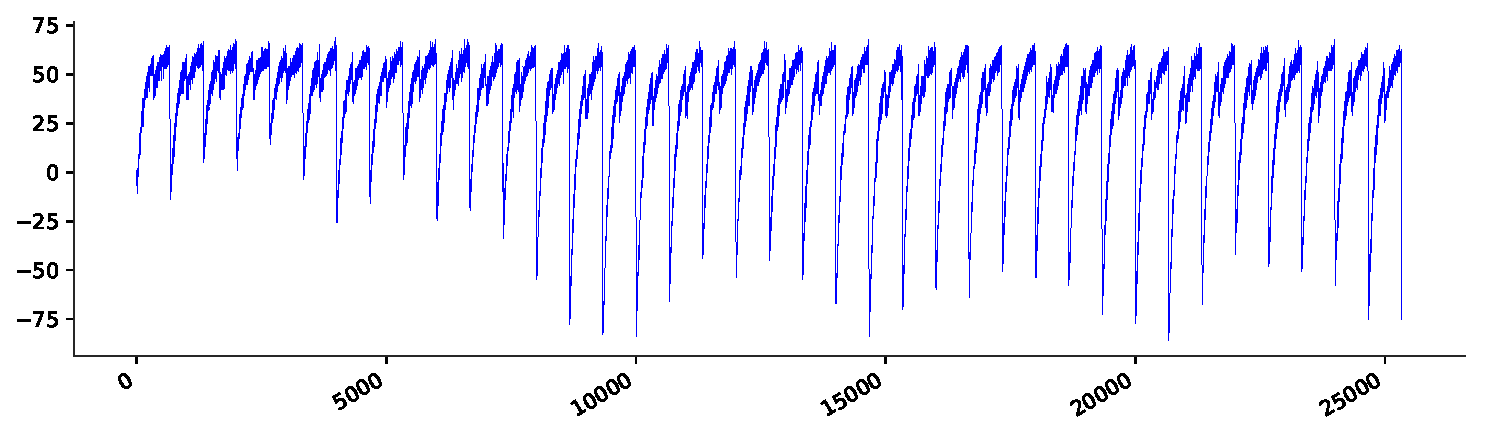
\includegraphics[scale=0.6]{traces/first_doubling/template_trace_dbl_oper_+d64_0}
	}
	\vfill
	\subfloat[$d_{64} = 1$]{
		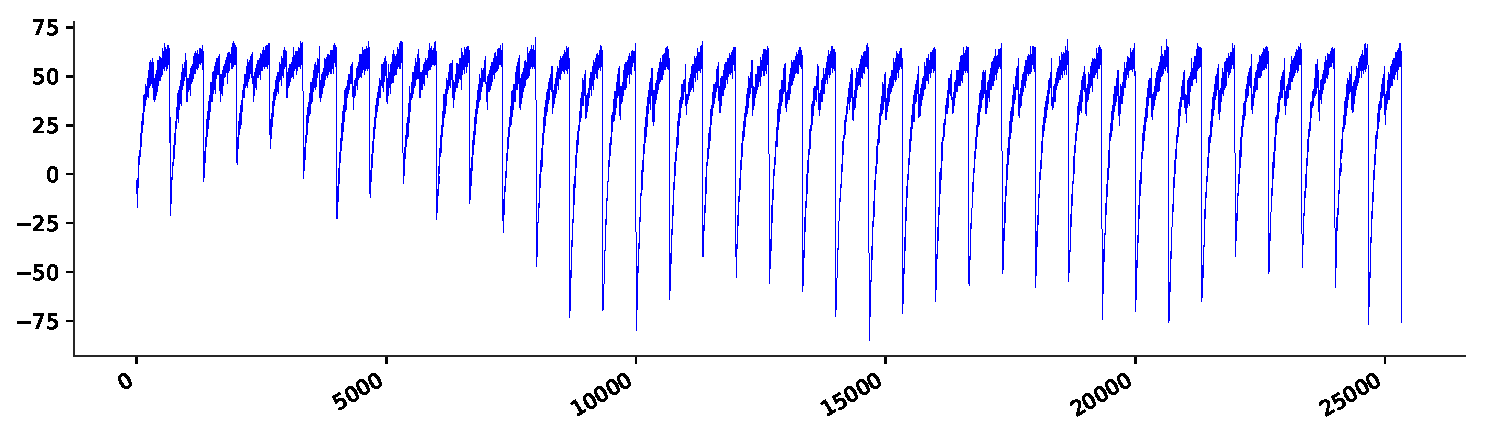
\includegraphics[scale=0.6]{traces/first_doubling/template_trace_dbl_oper_+d64_1}
	}
	\vfill
	\subfloat[$d_{64} = 2$]{
		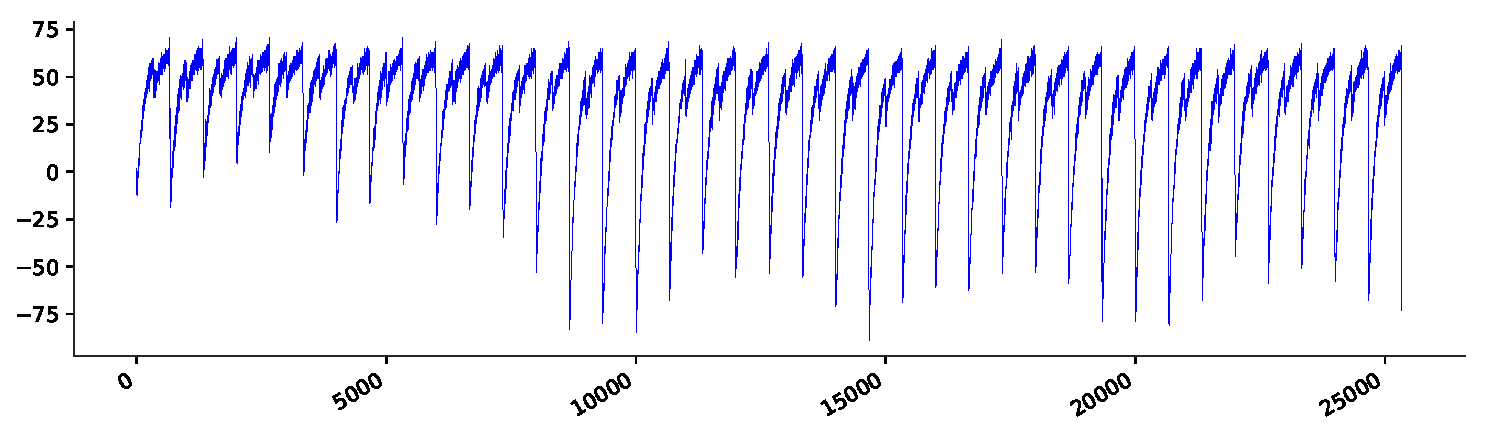
\includegraphics[scale=0.6]{traces/first_doubling/template_trace_dbl_oper_+d64_2}
	}
	\vfill
	\subfloat[$d_{64} = 3$]{
		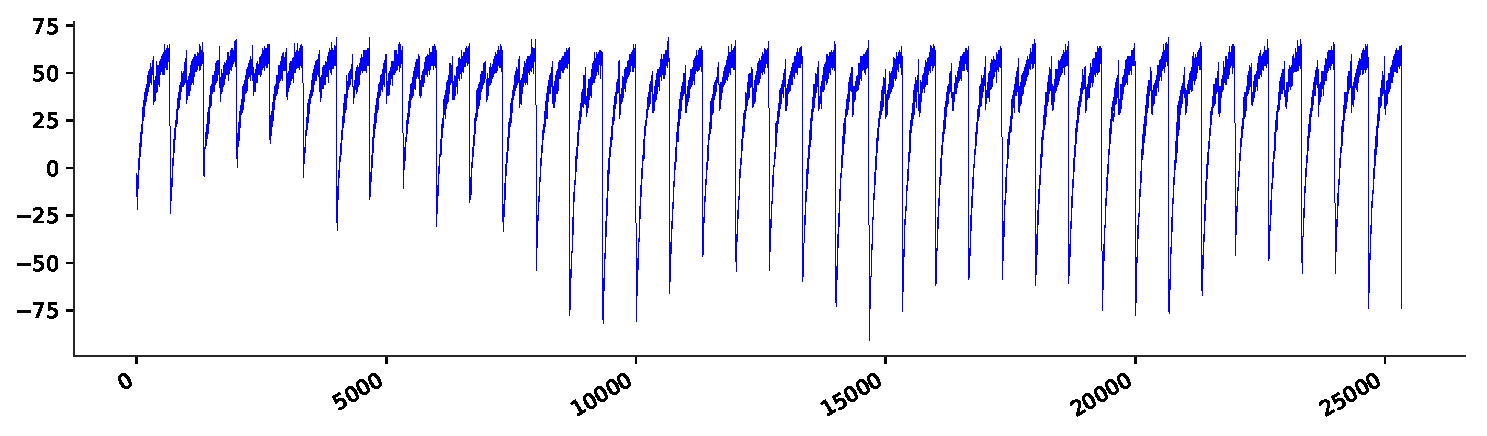
\includegraphics[scale=0.6]{traces/first_doubling/template_trace_dbl_oper_+d64_3}
	}
	\vfill
	\captionof{figure}{ }
\end{figure}
%
\begin{figure}\ContinuedFloat
	\centering
	\subfloat[$d_{64} = 4$]{
		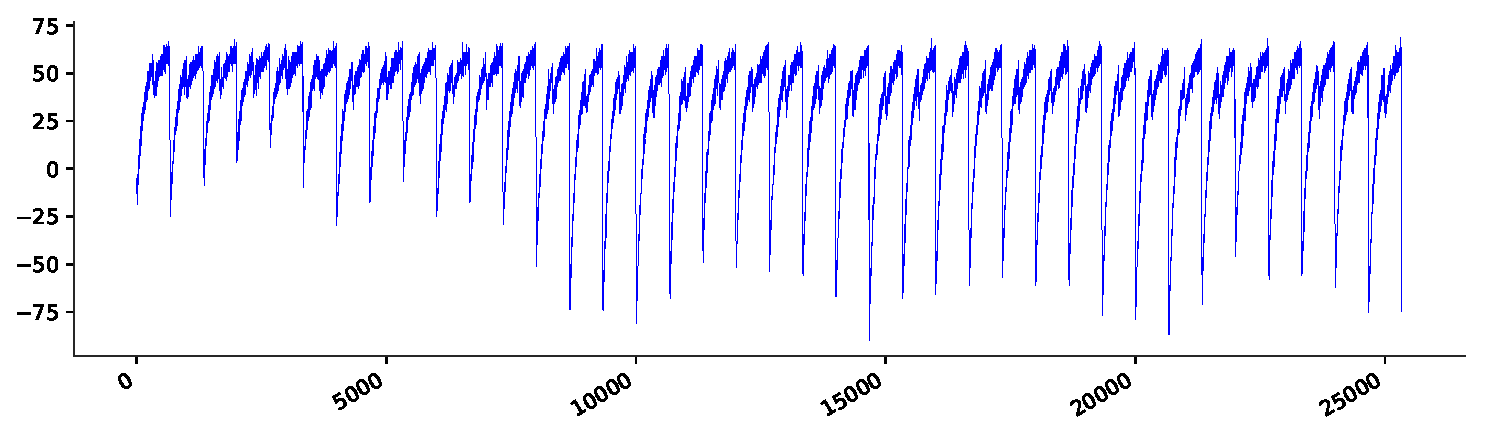
\includegraphics[scale=0.6]{traces/first_doubling/template_trace_dbl_oper_+d64_4}
	}
	\vfill
	\subfloat[$d_{64} = 5$]{
		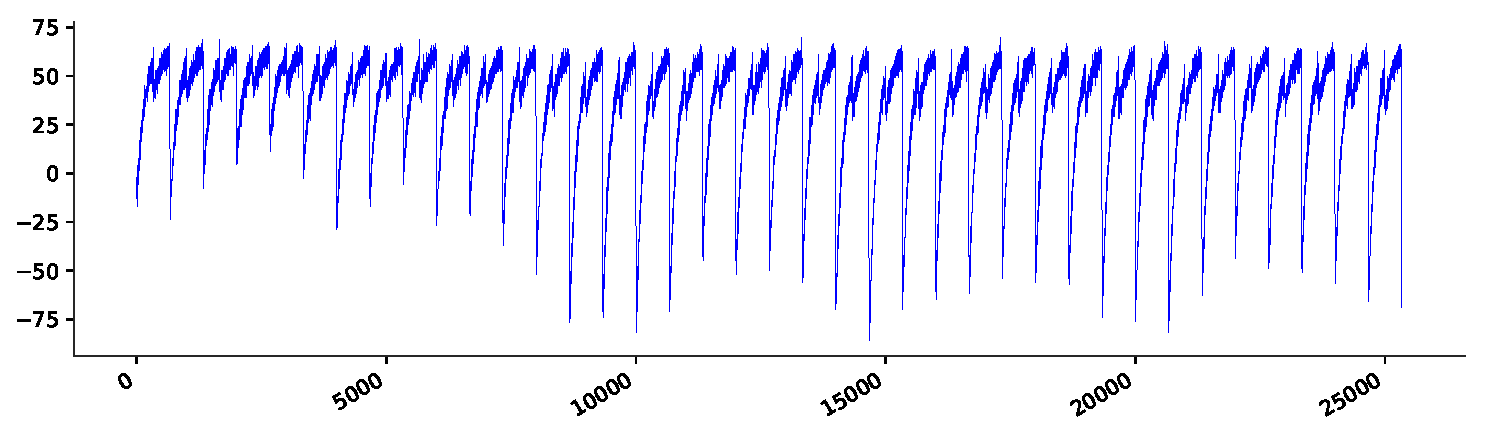
\includegraphics[scale=0.6]{traces/first_doubling/template_trace_dbl_oper_+d64_5}
	}
	\vfill
	\subfloat[$d_{64} = 6$]{
		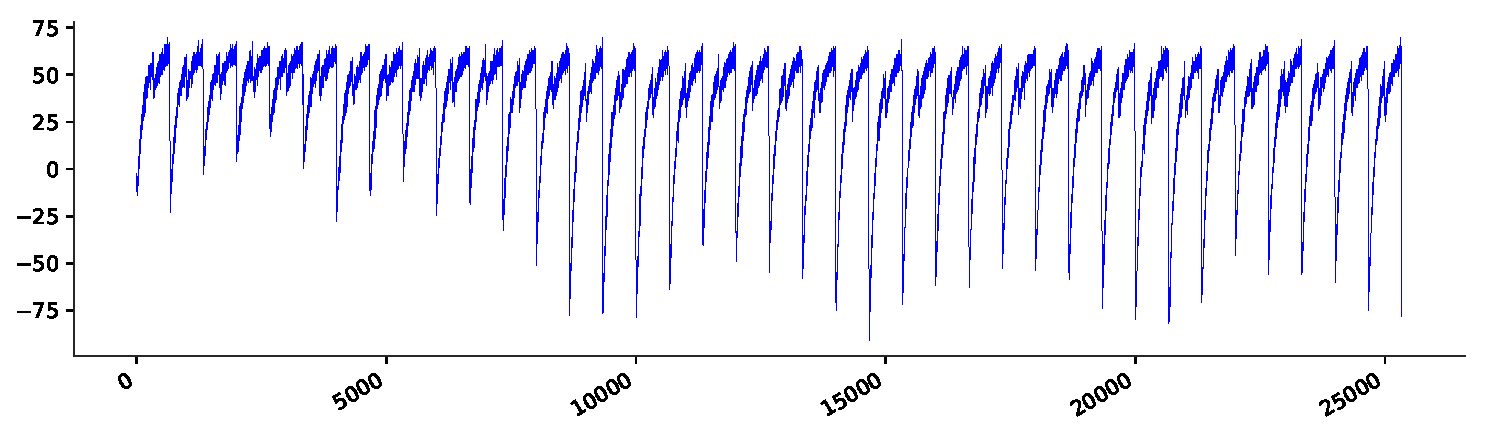
\includegraphics[scale=0.6]{traces/first_doubling/template_trace_dbl_oper_+d64_6}
	}
	\vfill
	\subfloat[$d_{64} = 7$]{
		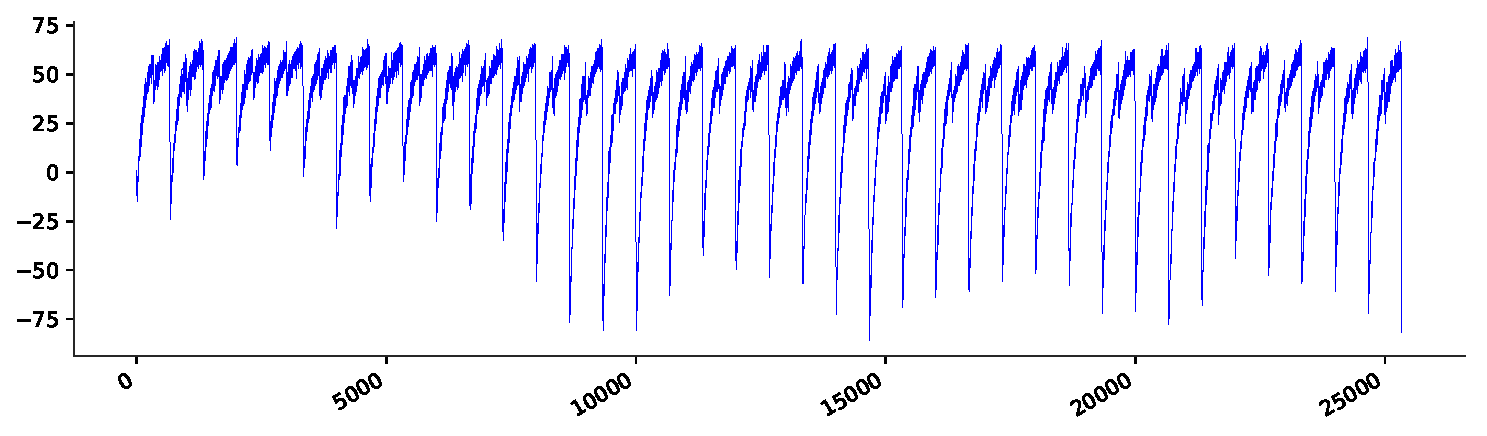
\includegraphics[scale=0.6]{traces/first_doubling/template_trace_dbl_oper_+d64_7}
	}
	\captionof{figure}{Template traces that are used to attack the first digit-column $d_{64}$ of {\fourq} using an Online Template Attack (OTA). The value of $d_{64}$ related to each template trace indicates that this was the specific value used in the doubling operation that resulted in the captured trace.}
	\label{fig: OTA first iteration templates example}
\end{figure}
%

\section{Measurement setup}
%
\begin{figure}[H]
	\centering
	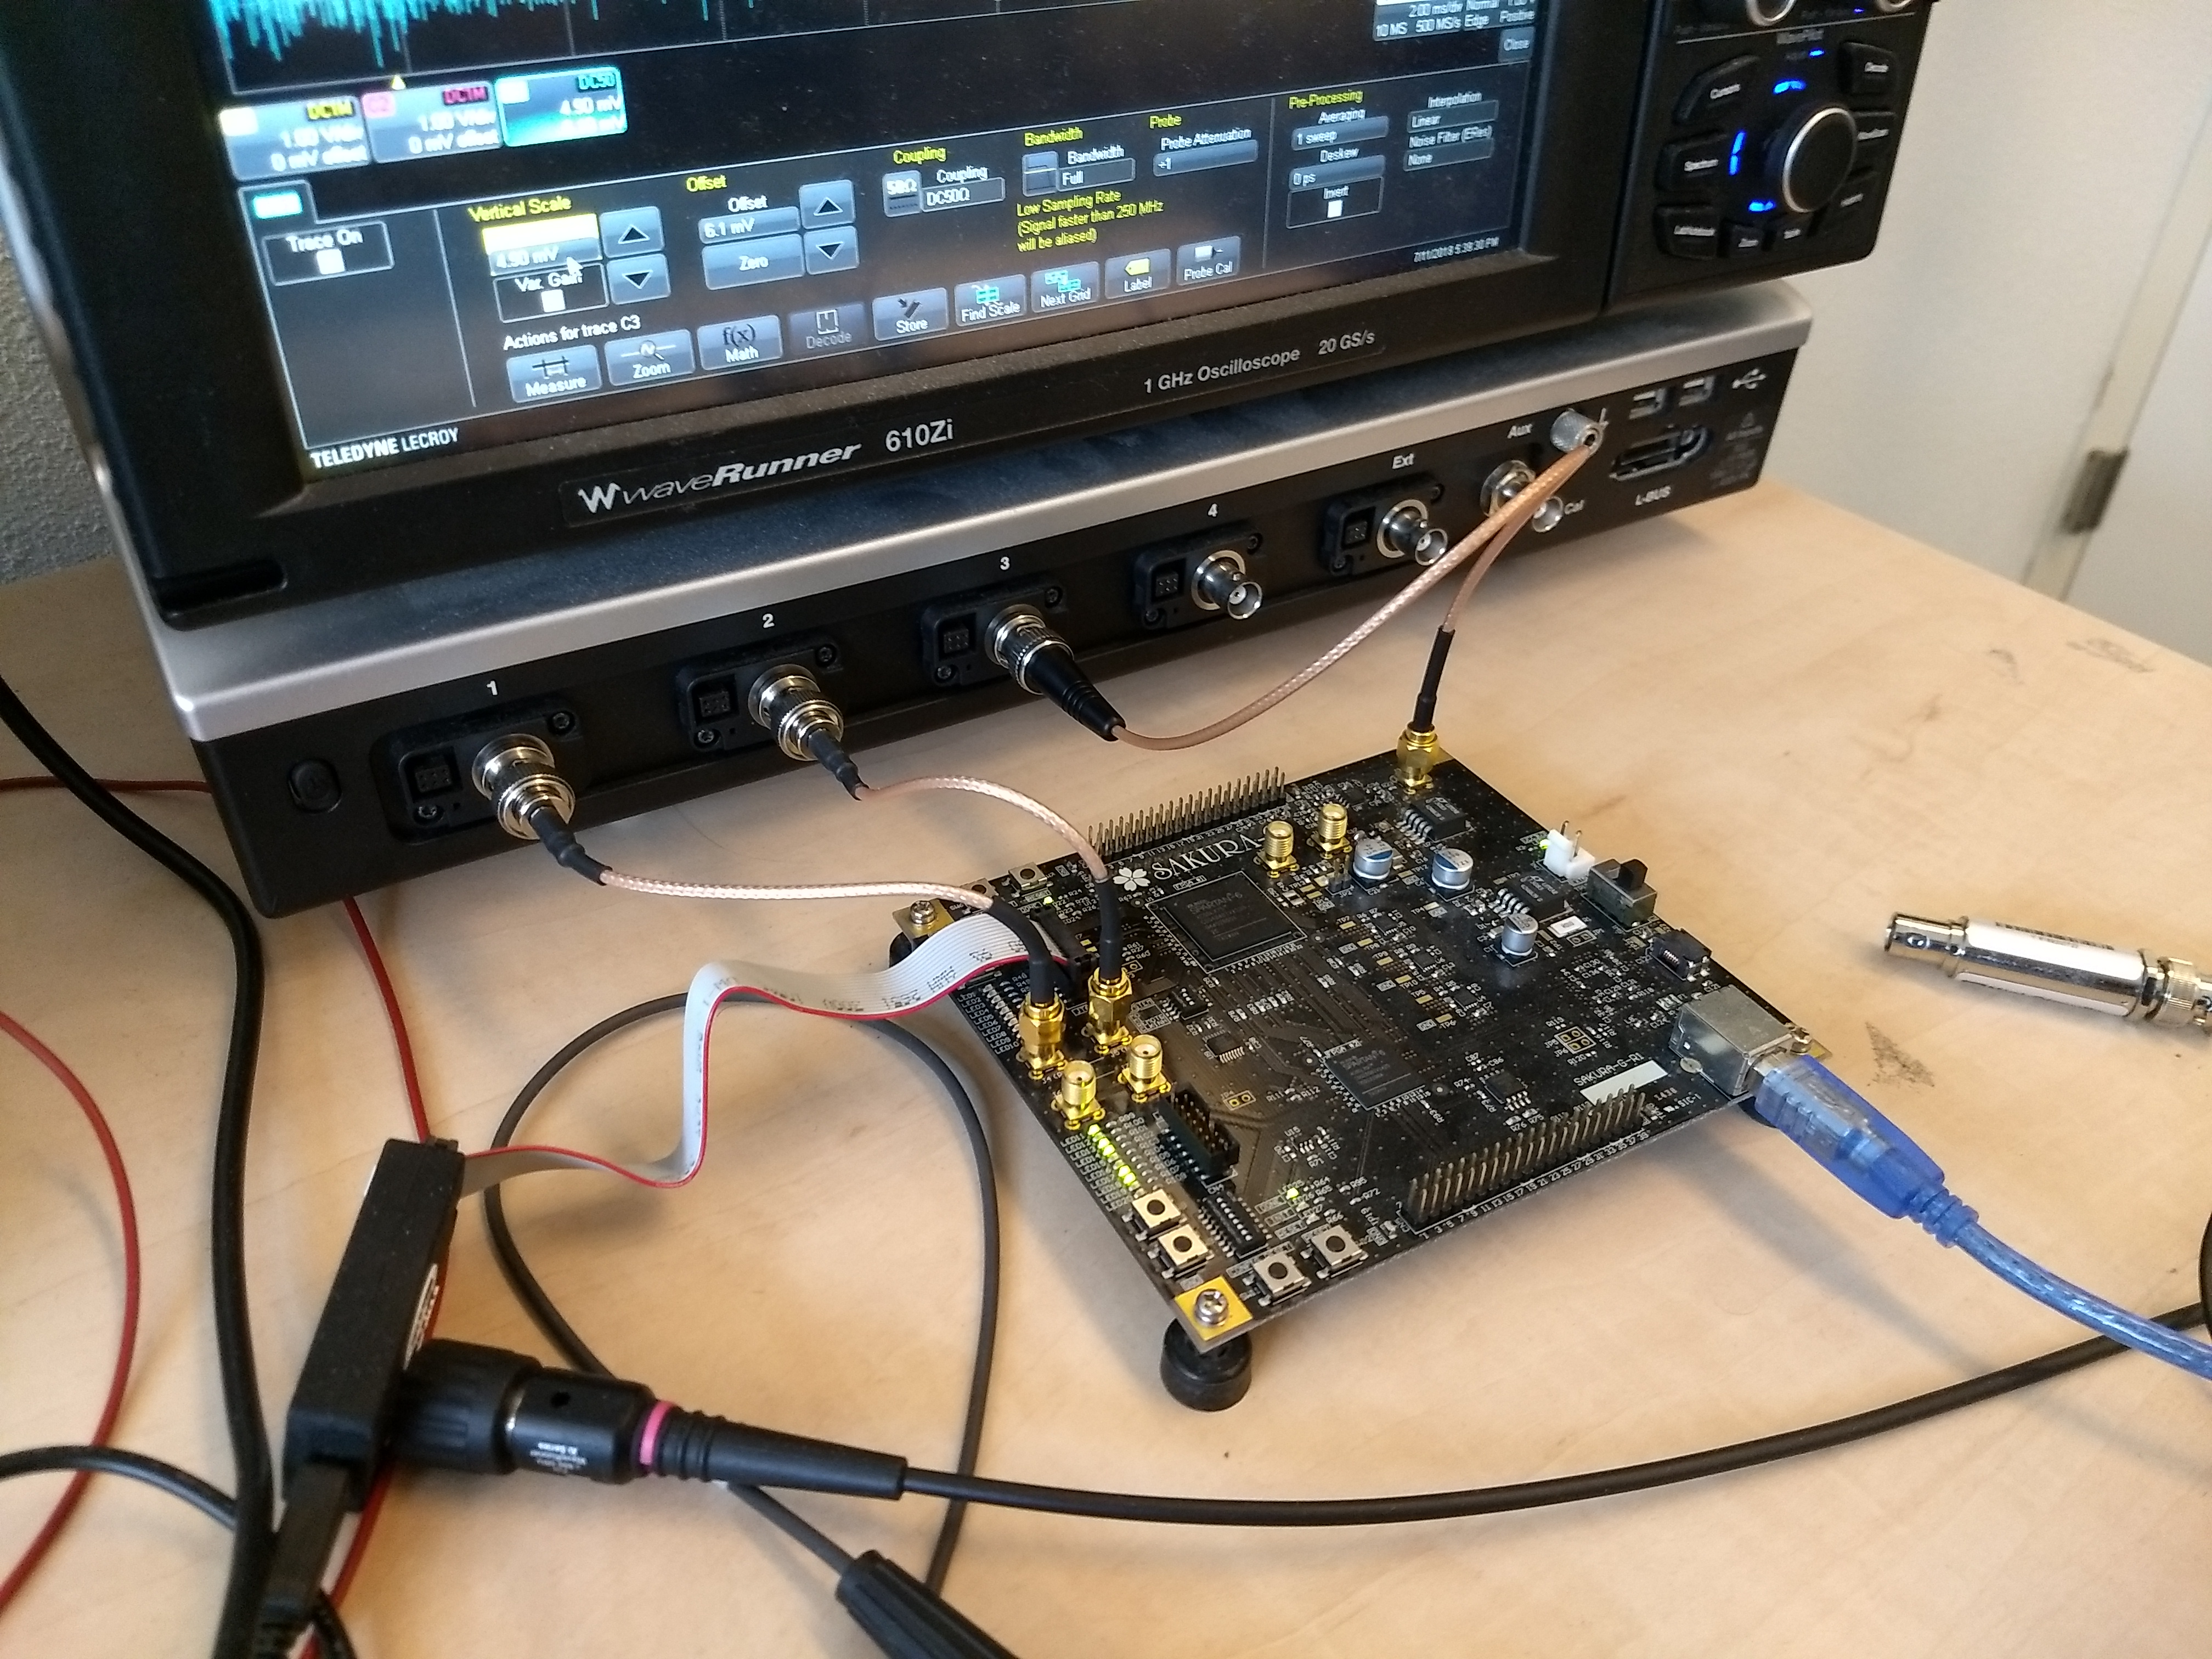
\includegraphics[scale=0.1]{setup/measurement_setup}
	\captionof{figure}{The measurement setup used to capture the power traces from the board. 
	The power output of the main FPGA is connected to $C_3$. The signal indicating the beginning and the end of the main loop is used as a trigger to capture all of the power traces. This trigger is assigned to $C_1$. Its trigger value is set to 1.00 V and it triggers on the positive edge of the signal. 
	The power trace that indicates the start and end of the doubling and addition operations in each iteration of the main loop in {\fourq} is obtained from $C_2$.
	The oscilloscope used during all of the acquisitions is the Teledyne LeCroy - WaveRunner 610Zi.
	}
\end{figure}
%


\end{document}